\expandafter\ifx\csname ifdraft\endcsname\relax
   \documentclass[a4j,12pt]{jsreport}
% 数式
\usepackage{amsmath,amsfonts}
\usepackage{bm}

% 画像
\usepackage[dvipdfmx]{graphicx}

% biblatex
\usepackage[style=numeric, sorting=none, maxbibnames=1000]{biblatex}
\addbibresource{graduation_thesis.bib}

%itembox
\usepackage{ascmac}
%breakitemboxのためのpackage
\usepackage{itembkbx}
% \usepackage{tcolorbox} 画像が見えなくなってしまう原因
% \usepackage{framed} 枠

%フォント
\usepackage[ipaex]{pxchfon}

\usepackage[top=35truemm,bottom=30truemm,left=30truemm,right=30truemm]{geometry}
\usepackage{float}
\usepackage{multicol}
\usepackage{paralist}
\usepackage{caption}
%\captionsetup{format=plain, justification=centering}
\usepackage{setspace}
\usepackage{algorithm}
\usepackage{algpseudocode}
\usepackage[dvipdfmx,hidelinks]{hyperref}
\usepackage{pxjahyper}
\usepackage{fancyhdr}
\usepackage{ltablex}
\usepackage{capt-of}
\usepackage{tabularx}
\usepackage{enumitem} % itemizeの行間 これは下になければならない
\usepackage{threeparttable} % 表の脚注


   \setlength{\headheight}{16.5pt}
   \captionsetup{format=hang}
   \begin{document}
   % 上部のヘッダー
\pagestyle{fancy}
\lhead{\rightmark}
\renewcommand{\chaptermark}[1]{\markboth{第\ \thechapter\ 章\ #1}{}}
\fi

\chapter{提案システム}\label{chap:proposedmethod}
本章ではまず, 本研究で開発したストーリー創作支援システムについて概要を述べる. 次に本システムが内部に持つプロンプトに関して筆者が行った提案について\ref{sec:prompt}節で述べ, 本システムに実装した4つの機能区分, プロット生成セクション, プロット編集セクション, シナリオ生成セクション, シナリオ編集セクションそれぞれについて, \ref{sec:plot_generation}節, \ref{sec:plot_edit}節, \ref{sec:scenario_generation}節, \ref{sec:scenario_edit}節において, その詳細と創作支援としての狙いを述べる. また, \ref{sec:implementation}節において, 本システムの実装における筆者の取り組みを述べる.

\section{概要}\label{sec:outline04}
図\ref{system}に本システムのイメージを示す. 本システムは, 図\ref{system}のようにストーリークリエータとLLMとの仲介役を担い, 御用聞きとして機能する.

\begin{figure}[H]
   \begin{center}
      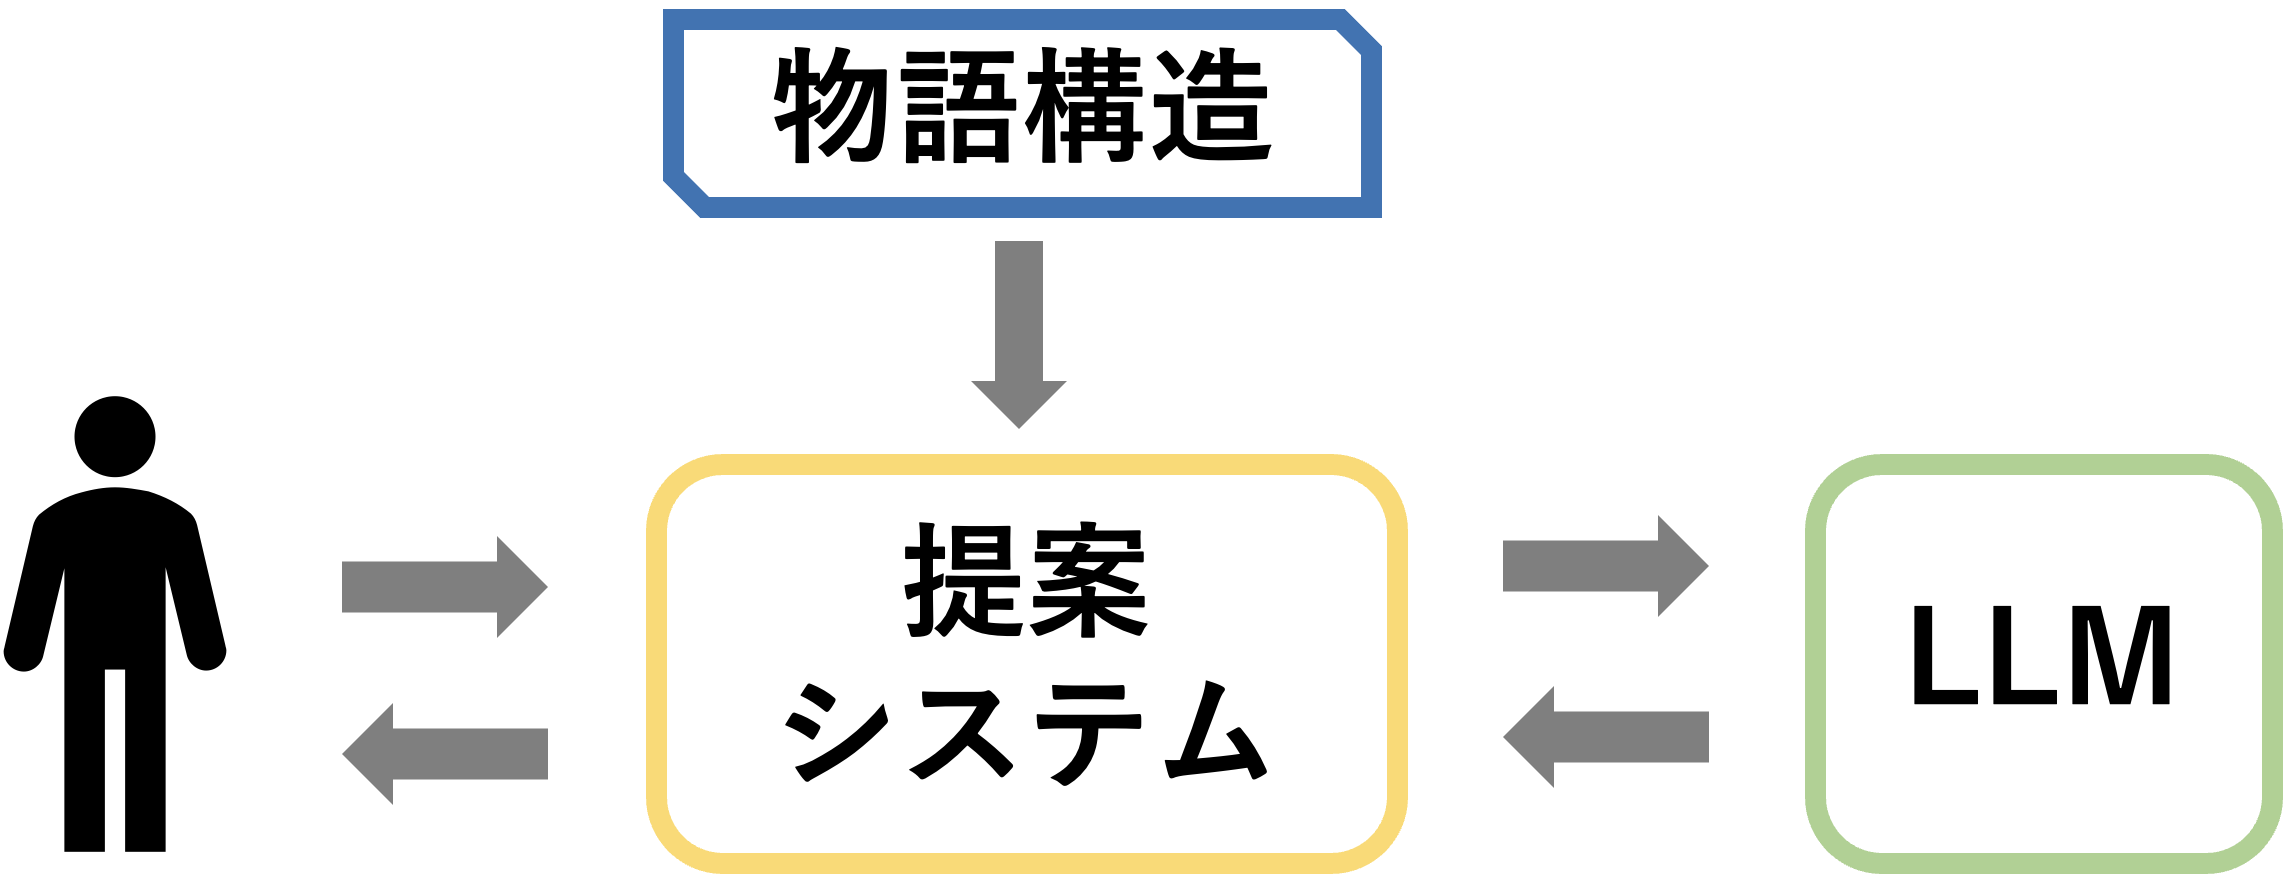
\includegraphics[width=5cm]{pict/04/system.png}
      \caption{提案システムのイメージ}
      \label{system}
   \end{center}
\end{figure}

本システムは, 手塚治虫の漫画『ブラック・ジャック』\cite{Tezuka77}における物語構造分析や, キャラクター分析により得られたデータをLLMの制御に活用することで, LLM とのインタラクティブな共創手法を提供し, 『ブラック・ジャック』の新作エピソード制作におけるストーリークリエーターの創作を支援する.

本システムにおいて実装した機能は大きく4つのセクションに分かれ, 一つは, ストーリーの骨格として活用される「プロット」の生成を行うセクション, 一つは, 生成したプロットのより洗練したものへの改変を支援するプロット編集セクション, 一つはプロット形式のストーリーを, ト書きと台詞からなる「シナリオ」へと変換するセクション, 一つは, プロット同様, より洗練したものへの改変を支援するシナリオ編集セクションである. いずれのセクションにおいても, ストーリークリエーターに向けたLLMの効果的かつ容易な活用を促すためのフレームワークを実装した. 本システムは, これらの機能を通じて, LLMを活用した, 物語構造分析に基づく『ブラック・ジャック』の新作エピソードのプロット生成, シナリオ生成を, 直感的な操作により実現するインターフェースとストーリーの洗練を目的としたLLMとのインタラクション手法を提供する. これらの実装を通じて, ストーリークリエーターの創作にかかる負担の軽減と創造的可能性を広げることを可能とし, ストーリー創作支援を実現する. 

本システムに接続したLLMはGPT-4である. \ref{ch:background}章で述べたとおり OpenAIが開発した GPT-4 はあらゆる自然言語処理タスクにおいて高い性能を発揮する\cite{OpenAI23}. API も公開されていることから, インターフェースへの接続も容易であり, 本システにムは GPT-4 を用いることとした.

\section{プロンプト}\label{sec:prompt}
本システムでは、ストーリークリエーターからの入力を受け取り, それらを内部で独自のプロンプトに整形する. そのプロンプトを LLM への入力とすることで, より効果的な出力を得られるようにしている. 筆者はプロットの生成に際して用いるプロンプトの叩き台を提案した. 本研究の取り組みでは, 筆者のプロンプトにさまざまな要素を加え, 洗練していくことで, より効果的なプロンプトを作成することを目指した. 叩き台として活用されたプロンプトにおいて, 筆者は本システムが活用する物語構造の展開要素の入れ込み方ついても提案しており, その入れ込み方は完成されたプロンプトにおいてもほとんど変わりなく使われている. 以下に筆者が提案した叩き台となったプロンプトを示す.

\begin{breakitembox}[l]{筆者が提案したプロンプトの叩き台}
      \noindent 状態が"状態1-\>状態2-\>状態3-\>状態4-\>状態5"と遷移する物語を生成してください。
ただし、下に示す情報を踏まえること。\\
1. 各々の状態は次の通りとする。\\
        \indent 状態1:  {[}世界観: {[}時代: 戦国時代{]}, {[}状態: 荒廃{]}{]},\\
               \indent \indent  {[}人物: {[}A: {[}役割: 主人公{]}, {[}職業: 剣士{]}, {[}性格: 勇敢{]}, {[}心情: 不安{]}{]}{]}\\
       \indent 状態2:  {[}世界観: {[}時代: 戦国時代{]}, {[}状態: 荒廃{]}{]},\\
               \indent \indent {[}人物: {[}A: {[}役割: 主人公{]}, {[}職業: 剣士{]}, {[}性格: 勇敢{]}, {[}関係: {[}B:友人{]}, {[}C: 敵対{]}{]}, {[}心情: 楽しい{]}{]},\\
                     \indent \indent  {[}B: {[}役割: ヒロイン{]}, {[}性格: 優しい{]}, {[}関係: {[}A: 友人{]}, {[}C: 嫌悪{]}{]}{]},\\
                     \indent \indent  {[}C: {[}役割: ライバル{]}, {[}職業: 剣士{]}, {[}性格: 傲慢{]}, {[}関係: {[}A: 敵対{]}, {[}B: 片思い{]}{]}{]}{]}\\
       \indent 状態3:  {[}世界観: {[}時代: 戦国時代{]}, {[}状態: 荒廃{]}{]},\\
               \indent \indent {[}人物: {[}A: {[}役割: 主人公{]}, {[}職業: 剣士{]}, {[}性格: 勇敢{]}, {[}関係: {[}B: 友人{]}, {[}C: 敵対{]}{]}, {[}心情: 苦悩{]}{]},\\
                \indent \indent       {[}B: {[}役割: ヒロイン{]}, {[}性格: 優しい{]}, {[}関係: {[}A: 友人{]}, {[}C: 嫌悪{]}{]}{]},\\
                     \indent \indent  {[}C: {[}役割: ライバル{]}, {[}職業: 剣士{]}, {[}性格: 傲慢{]}, {[}関係: {[}A: 敵対{]}, {[}B: 片思い{]}{]}{]}{]}\\
      \indent  状態4:  {[}世界観: {[}時代: 戦国時代{]}, {[}状態: 荒廃{]}{]},\\
               \indent \indent {[}人物: {[}A: {[}役割: 主人公{]}, {[}職業: 剣士{]}, {[}性格: 勇敢{]}, {[}関係: {[}B: 友人{]}, {[}C: 敵対{]}{]}, {[}心情: 歓喜{]}{]},\\
                  \indent \indent {[}B: {[}役割: ヒロイン{]}, {[}性格: 優しい{]}, {[}関係: {[}A:友人{]}, {[}C: 嫌悪{]}{]}{]},\\
                  \indent \indent {[}C: {[}役割: ライバル{]}, {[}状態: 死亡{]}{]}{]}\\
      \indent  状態5:  {[}世界観: {[}時代: 戦国時代{]}, {[}状態: 平和{]}{]},\\
               \indent {[}人物: {[}A: {[}役割: 主人公{]}, {[}職業: 剣士{]}, {[}性格: 勇敢{]}, {[}関係: {[}B: 恋人{]}, {[}C: 敵対{]}{]}, {[}心情: 安心{]}{]},\\
                  \indent \indent     {[}B: {[}役割: ヒロイン{]}, {[}性格: 優しい{]}, {[}関係: {[}A: 恋人{]},{[}C: 嫌悪{]}{]}{]},\\
                     \indent \indent  {[}C: {[}役割: ライバル{]}, {[}状態: 死亡{]}{]}{]}\\
2. それぞれの状態遷移は次のテーマを持つものとする。\\
      \indent  {[}状態1-\>状態2{]}: 出会い\\
      \indent  {[}状態2-\>状態3{]}: 決意\\
      \indent  {[}状態3-\>状態4{]}: 対決\\
      \indent  {[}状態4-\>状態5{]}: 平穏\\
3. 出力は次のような形式とすること。\\
      \indent  {[}状態1-\>状態2{]}\\
      \indent  (本文)\\
      \indent  {[}状態2-\>状態3{]}\\
      \indent  (本文)\\
      \indent  {[}状態3-\>状態4{]}\\
      \indent  (本文)\\
      \indent  {[}状態4-\>状態5{]}\\
      \indent  (本文)\\
4. (本文)はそれぞれ200文字以上400文字以下とすること。\\
5. {[}状態3-\>状態4{]}には次の状況を含めること\\
      \indent  AがCを崖から突き落とす
   \end{breakitembox}
\vspace*{-6pt}
\begingroup
\captionof{figure}{筆者が提案したプロンプトの叩き台}
\label{prompt_base}
\endgroup

\section{プロット生成セクション}\label{sec:plot_generation}
ここでは, 本システムにおいて実装した機能区分, プロット生成セクションについて述べる. 本セクションでは, 図\ref{flow}に示すフローに従い操作を進めることで, LLMを活用しながら, 『ブラック・ジャック』の物語構造分析に基づきプロットの生成を行うことができる. 図\ref{flow}に示すフローをガイドラインとして進めるだけでプロットを生成することができ, AIの理解度に依存しない, LLM の効果的活用を促すものである.

\begin{figure}[hbtp]
   \begin{center}
   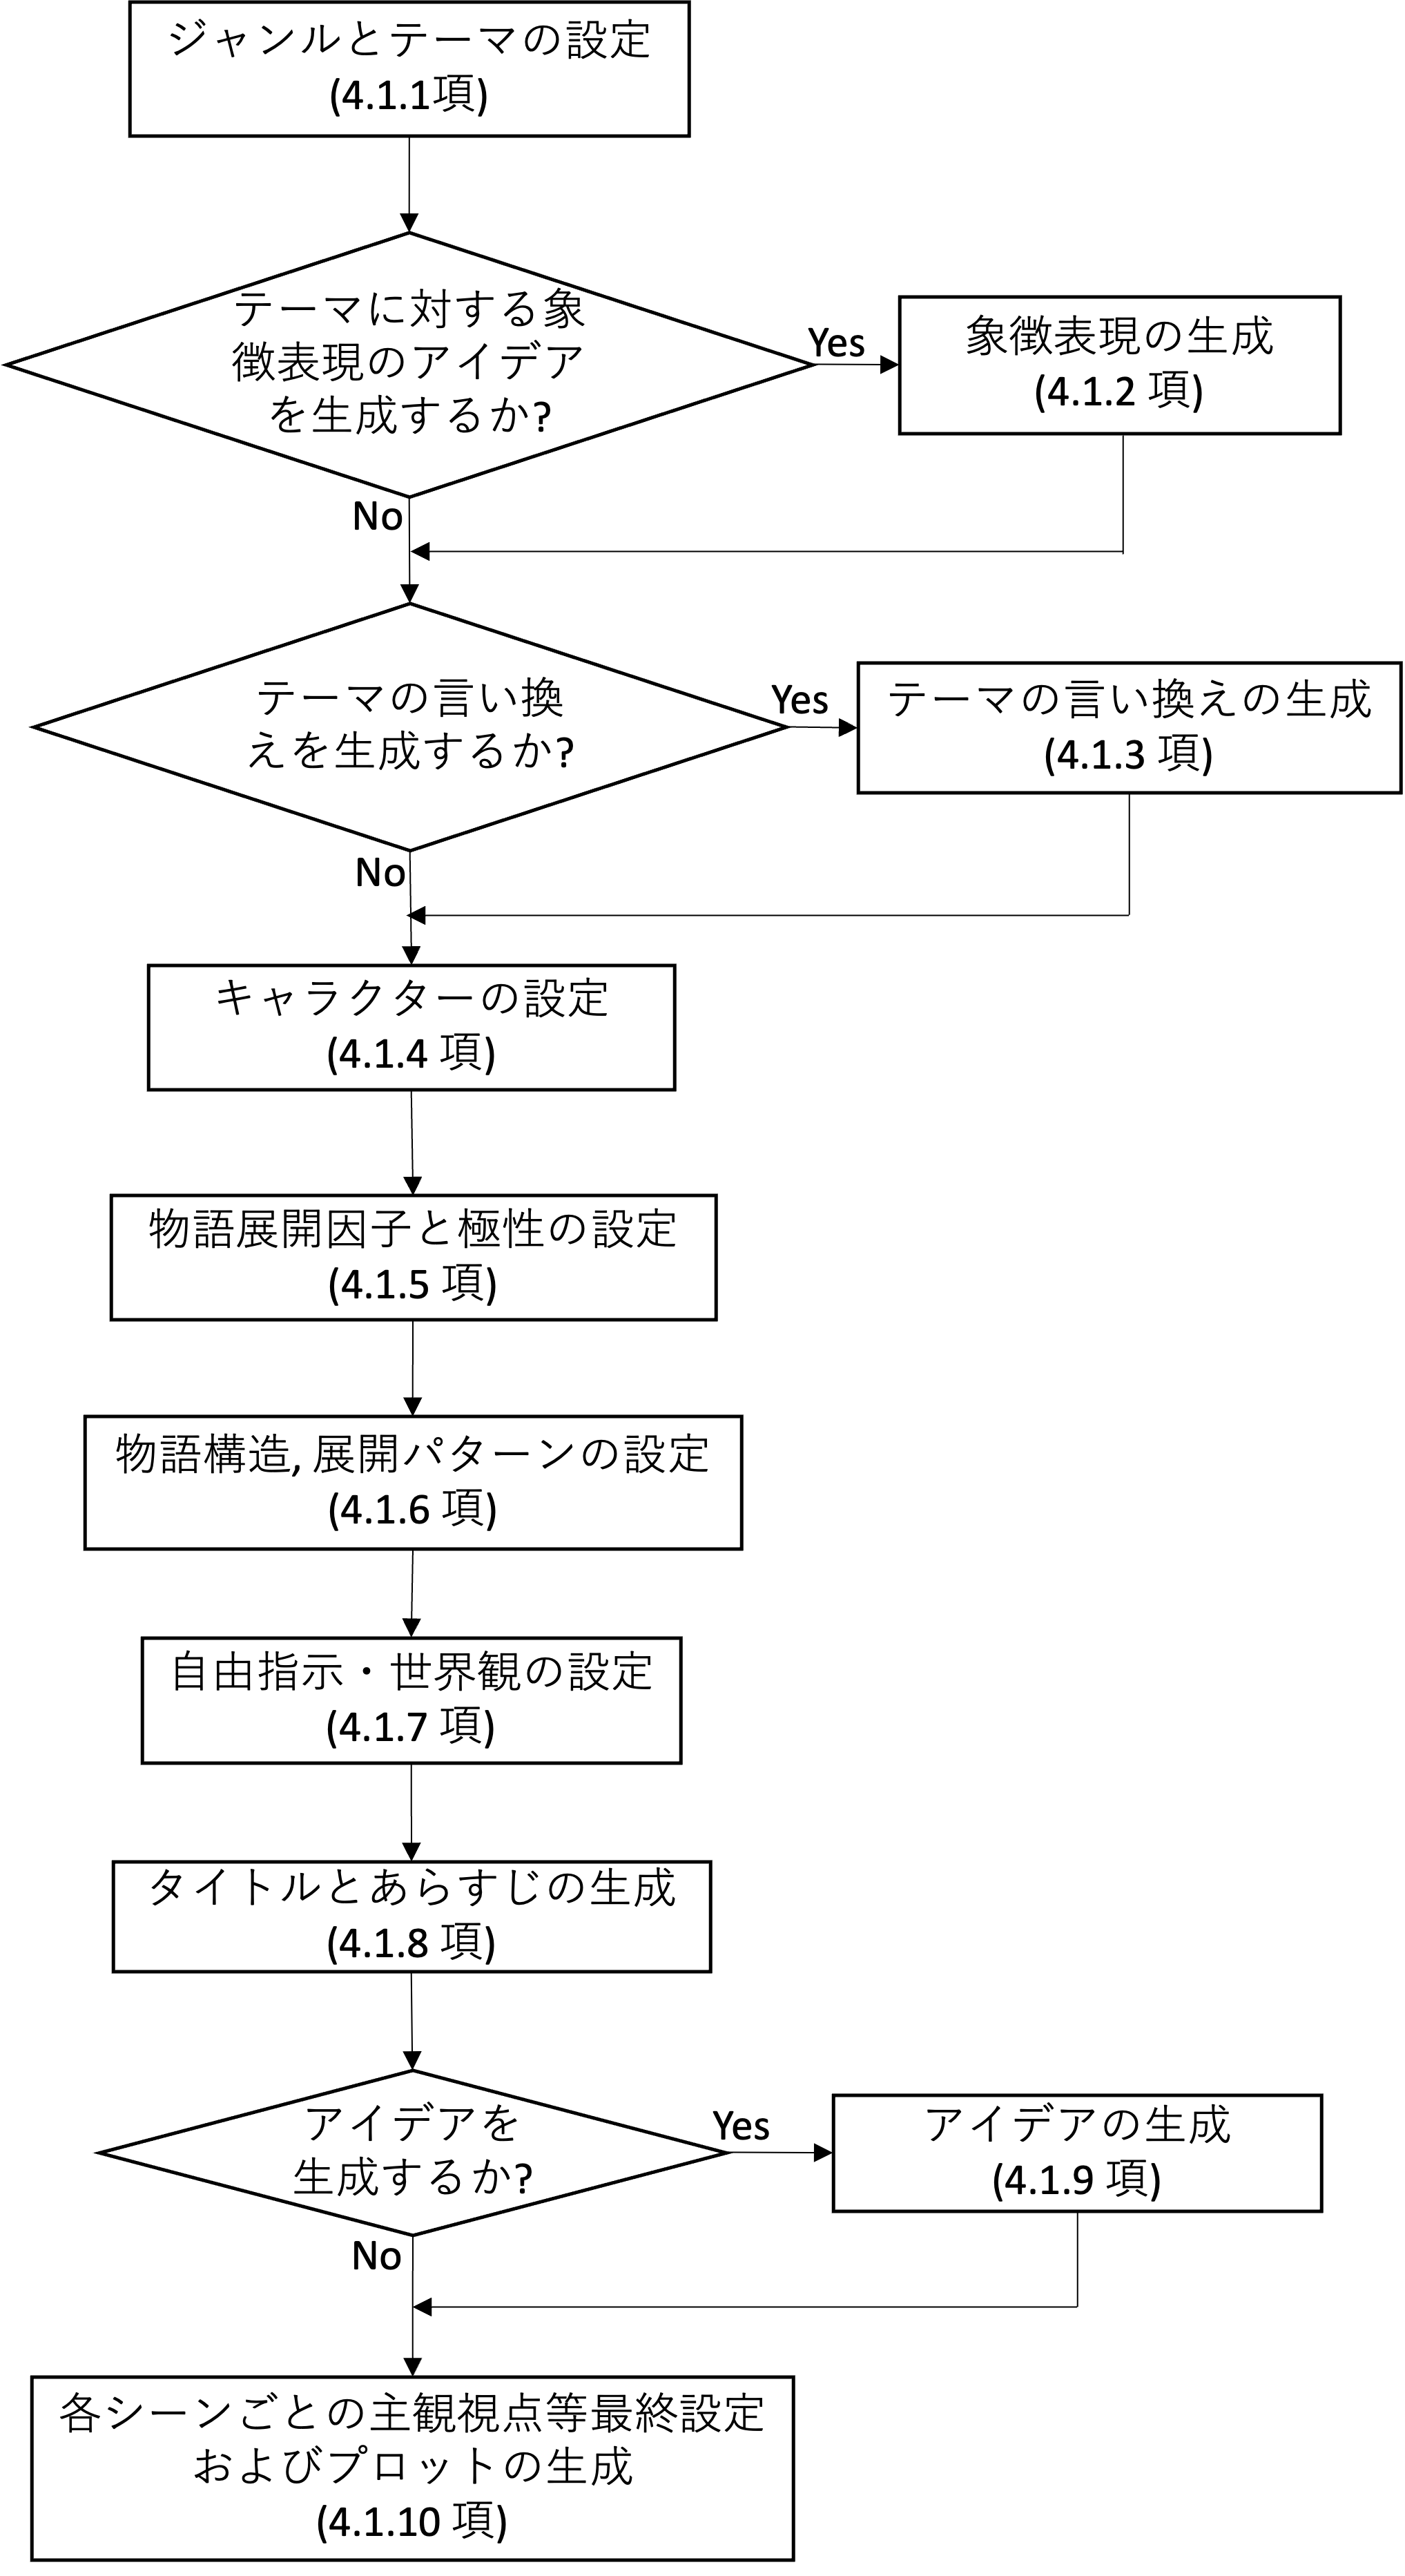
\includegraphics[width=5cm]{pict/04/flow.png}
   \caption{プロット生成セクションにおけるフロー.}
   \label{flow}
   \end{center}
\end{figure}


図\ref{flow}のフローで示したいずれのステップにおいても操作は簡潔で, 画面の指示に従う直感的な操作, 選択と入力を行うことにより, 容易に次のステップへと移行できるようになっている. 画面の誘導に従い, 図\ref{flow}に示したフローの先へと操作を進めていくことで, プロットの生成に際しLLMの制御として効果を持ち得る物語の設定を, LLMを活用しながら簡便に定めることができる. これによりストーリークリエーターの負担を軽減する. また, 『ブラック・ジャック』の物語構造分析により得られたデータをそれぞれのステップにおいて提示し, これらの活用を促すことで, 『ブラック・ジャック』の新作エピソードの骨格となるプロットとしての整合性を担保するとともに, ストーリー創作におけるアイデアを生み出す手間の削減とストーリークリエーターの創造性の刺激とする.

ここでいうプロットとは, 物語の全体的な流れを表す文章のことである. プロットには, 物語の中で起こる主要な出来事や重要な展開, さらには, 登場人物たちの物語上における役割やそれに応じた彼らの大まかな動き, 変化などが含まれる. プロットは, 物語の全体的な構造や進行を文章という形で視覚化するものであり, ストーリークリエーターは, このプロットを通じて物語の全体像を把握することができる. 

本システムで生成することができるプロットは, 1000字から2000字程度の長さをもつプロットであり, この範囲のプロットには物語の骨格となる要素が十分に含まれ, 『ブラック・ジャック』の新作エピソード制作において, その基盤となる役割を果たす.

% 生成されるプロットの例の図を入れる

本システムにおける第一段階の生成物として, 物語そのものではなくそのプロットを生成するようにしたことは, 次に述べる二つの理由による. 一つは, 物語そのものには物語構造の上に演出上のカスタマイズがなされるため, 物語構造分析を活用したLLMの制御を直接活かすことができないと考えられること. もう一つは, 本システムがクリエーターの代替となることを目的として開発されたものではなく, クリエーターの創作支援となることを目的として開発されたものであるため, 創造性を掻き立てる形式としてプロットという形式が望ましいと考えたためである.

以下では, 図\ref{flow}に示したフローに従い, プロット生成セクションの各ステップにおける, 操作と創作支援としてのねらいについて述べる.

\subsection{ジャンル・テーマの設定}
このステップでは, 物語のジャンルおよびテーマを, 『ブラック・ジャック』の分析により得た, 「SF」や「人間ドラマ」など, ジャンル64種と, 「親子愛」や「友情」など, テーマに関するキーワード152種の中から複数選び設定することができる. 図\ref{genre}にジャンルの設定画面の様子を示す. ジャンルの設定画面は図\ref{genre}のようになっており, ユーザーは画面に表示されるジャンルの一覧から最大で3つ, 生成するプロットのジャンルをクリック操作のみで選択することができる. 

\begin{figure}[hbtp]
   \begin{center}
   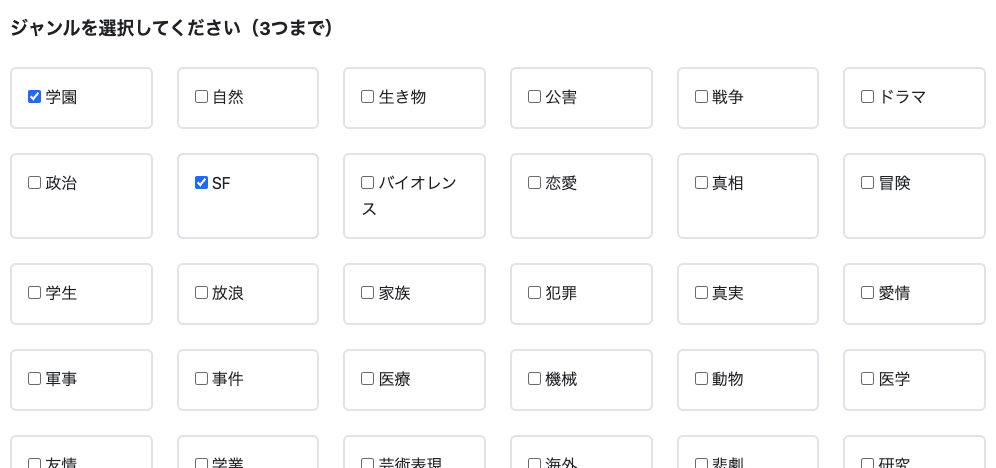
\includegraphics[width = 12cm]{pict/04/genre01.png}
   \caption{ジャンルの設定画面}
   \label{genre}
   \end{center}
\end{figure}

%ジャンルとは
物語におけるジャンルとは, その作品の全体的な色や雰囲気をもとに区別される物語の種類, 分類のことであるといえる. 例えば, Geduld\cite{geduld73}らは, 著書『An Illustrated Glossary of Film Terms\footnotemark \footnotetext{\url{https://books.google.co.jp/books/about/An_Illustrated_Glossary_of_Film_Terms.html?id=W4JZAAAAMAAJ&redir_esc=y} (cited 2024-01-27)}』の中で, ジャンルのことを"主題やテーマ, 技法によって区別されるカテゴリー, 種類, 形式のことである"と定義しており, これは映画におけるジャンルの定義ではあるが, この定義をとりわけて映画作品だけのものとして物語全般の話から区別する必要はないと考えられる. つまり, ジャンルはその作品がどのような作品であるかを定める際に用いられる区分であり, このような区分を定めておくことは, ストーリーの創作において大きな指針になり得ると考えられる.

物語作品には唯一のジャンルが定められるわけでなく, その作品の中には複数のジャンルが含まれることがある. 例えば, 『ブラック・ジャック』には「SF」と「人間ドラマ」の要素を同時に含む回が存在する. Daiku\cite{daiku17}らは, 漫画作品において, ページごとに畳み込みニューラルネットワーク\cite{CNN}を用いてジャンルを分類し, ジャンルのシーケンスとしてその作品の物語構造を分析するといった研究を行った. 作品を複数ジャンルの複合として紐解くことで, 作品世界の理解が深まると考えられる. つまり, 物語創作においては, 創作する漫画を複数ジャンルの複合として定めておくことで, 創作する作品の理解度および解像度が高まり, これは創作支援になると考えられる.

本システムでは, 生成するプロットのジャンルの設定として, 『ブラック・ジャック』の分析により得たジャンル64種の中から最大3つの選択を可能とした. 設定できるジャンルを最大で3つとした理由は, 『ブラック・ジャック』の物語構造分析において, いずれのエピソードにおいても当てはめるジャンルの数として最大3つが適切であると考えられたためである.

ジャンルという, 物語作品の枠組みとして創作の指針となり得る有用な設定を, 物語構造分析により得られたデータからクリック操作のみで簡便に定められるシステムは, ストーリークリエーターの創作支援に役立つものと考えられる.

ジャンルの一覧は, 付録\ref{appendix:genre_list}に示す.

テーマの選択画面は図\ref{theme}のようになっている.

\begin{figure}[H]
   \begin{center}
   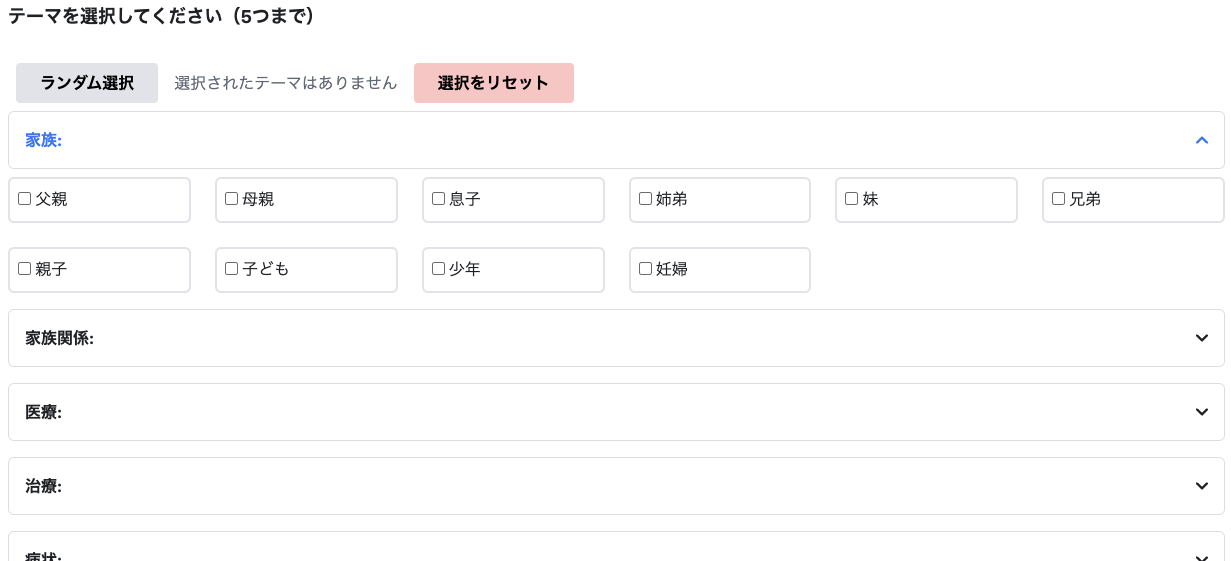
\includegraphics[width = 12cm]{pict/04/theme02.png}
   \caption{テーマの設定画面}
   \label{theme}
   \end{center}
\end{figure}

ここでいうテーマとは, 物語作品を通して伝えられるメッセージや考えの提示であり, 物語の中心となるものである. 例えば, 『ブラック・ジャック』のエピソードの中には, テーマに「生と死」を含むエピソードがある. このエピソードの中では, 「生と死」に関する様々な問題が取り上げられ, それらの問題に対する答えが提示されることで, 作品全体を通し「生と死」について考えさせられるようになっている. このように, 物語のテーマは, 物語の中心となるものであり, 物語の中で起こる出来事や登場人物の行動は, そのテーマを伝えるための手段として機能する. 物語のテーマは, 物語上の様々な要素を決定する上で重要な役割を果たすものであるといえる. 

このように物語の中心となるテーマを, 図\ref{theme}で示したように, 『ブラック・ジャック』の物語構造分析により得られたテーマから, クリック操作のみで簡便に定めることができるシステムは, ストーリークリエーターの創作支援に役立つものと考えられる.

『ブラック・ジャック』の分析により得られたテーマは152種と多岐にわたるため, 次表\ref{theme_list}に示す 21 のカテゴリに分類し, それぞれのカテゴリに分けてテーマを表示することで, ユーザーが選択しやすいよう工夫を施した.

このカテゴリは, SentenceBERT\cite{SBERT} を用い, コサイン類似度が 0.7 以上のものを同じカテゴリとして分類した結果である.

%テーマ一覧
\setlongtables
   \begin{tabularx}{\textwidth}{l|X}
   \caption{テーマ一覧 \label{theme_list}}
   \vspace*{-5pt}
      \endfirsthead
   \hline
   カテゴリ & テーマ \\
   \hline
   家族 & 父親, 母親, 息子, 姉弟, 妹, 兄弟, 親子, 子ども, 少年, 妊婦 \\
   家族関係 & 息子思い, 親子愛, 家族愛, 親孝行, 兄弟愛 \\
   医療 & 医者, 手術, 医学, 輸血, 医学研究, 研究, 誤診, 整形手術 \\
   治療 & 治療, 荒療治, リハビリ \\
   病状 & 大怪我, 障害, 盲目 \\
   金 & 金, 金と命, 治療費, 寄付 \\
   地位 & 権力者, 人気者, お金持ち, 権力, 名誉 \\
   生と死 & 生命, 生と死, 安楽死, 生きがい, 自殺, 自殺未遂 \\
   事件・事故 & 戦争, 人質, 脅迫, 事故, 交通事故, 飛行機事故, 殺人, 殺人未遂 \\
   アウトロー & 裏社会, 犯罪, 暴力, 強盗, 悪巧み, 禁忌 \\
   教育・指導 & 教師, 助手, 恩師 \\
   人間関係 & 友情, 協力, 信頼関係, 憧れ, 信頼, 尊敬, 裏切り, 対立, 人間関係, 友だち, 恋人 \\
   心情 & 執念, 信念, 願望, 情熱, 思いやり, 反抗心, 意地, 愛情, 嫉妬, 覚悟, 怒り, 感謝, 諦め, 葛藤, 迷い, 苦悩, 悲しみ, 絶望, 後悔 \\
   道徳 & 人情, 人助け, 励まし, 思いやり, 手助け, 愛情 \\
   出来事 & 再会, 別れ, 危機一髪, 挫折, 失敗, 真似事 \\
   希望的展開 & 成長, 回復, 新発見, 希望, 再出発 \\
   社会問題 & 貧困, 孤児, 孤独 \\
   主義・概念 & 自由, 正義, 存在意義, 真実 \\
   トピック & メッセージ, 告白, 約束, 秘密, 嘘, 矛盾, 誤解 \\
   行動 & 探索, 演技, 通報, 野宿, 機転 \\
   時間軸 & 過去, 未来 \\
   \hline
\end{tabularx}

ユーザーは, 図\ref{theme}のように, まずはテーマのカテゴリを選択する. すると, そのカテゴリに属するテーマが表示されるので, その中からテーマに関するキーワードを選択することができるようになる. 

分析に基づいた選択肢をあらかじめ用意し, 簡便な操作によりテーマを設定できるシステムは, 創作の手間を削減すると考えられ, また, 多岐にわたるキーワードの提示は, 創作におけるアイデアへの刺激につながるものと考える.

選択は, 自身の意思により行うこともできれば, ランダム選択機能を用いて行うこともできる. 選び取る時間の削減とランダムネスによる創造性支援を行う\cite{Osone21}.

\subsection{象徴表現の生成}
ここでは, 選択したテーマや自身で考えたテーマに関するキーワードからその象徴表現を, LLM を介して生成することができる. 

ここでいう象徴表現とは, 平和という概念を鳩を用いて表すように, 抽象的な概念を別のものに置き換え表す表現技法のことである. この表現技法は, 小説や映画, 詩など様々な場面に用いられ, 物語に何層もの意味を加えて作品を豊かにするのに役立つものである\cite{Norva23}.

\begin{figure}[hbtp]
   \begin{center}
   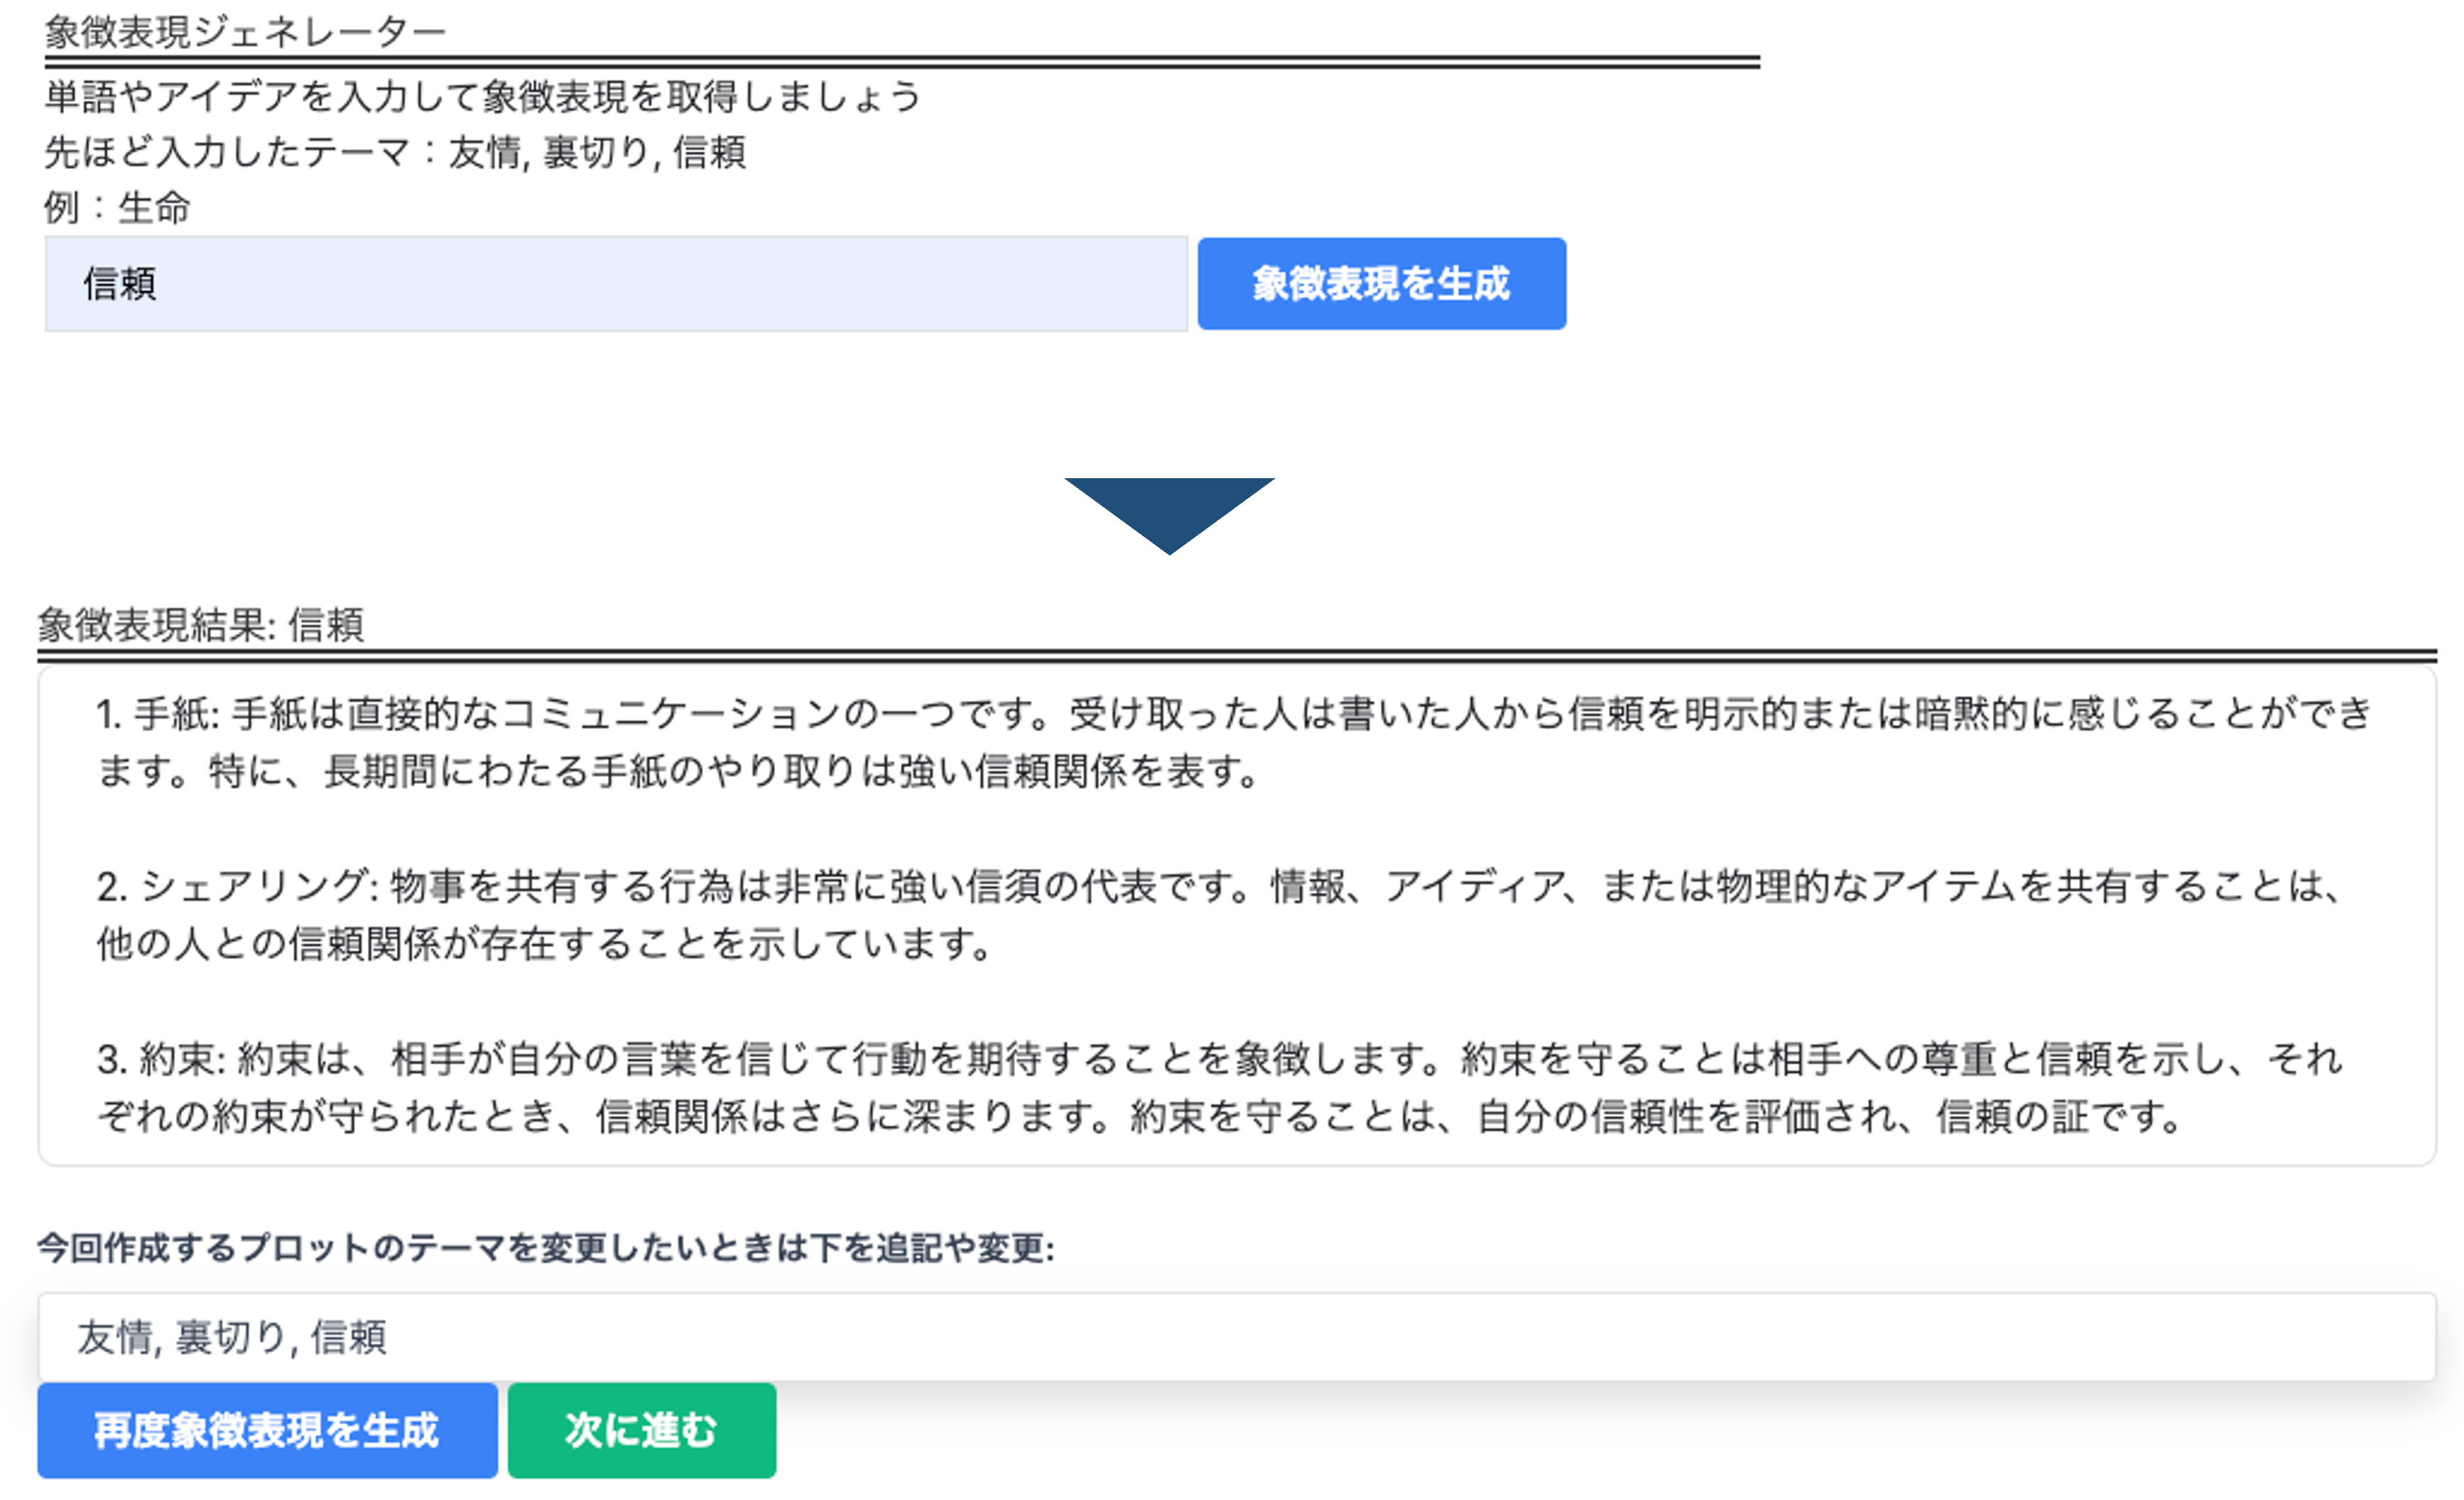
\includegraphics[width = 12cm]{pict/04/symbol.png}
   \caption{象徴表現を生成する画面の様子}
   \label{symbol}
   \end{center}
\end{figure}

図\ref{symbol}で示したのは, 本システムで象徴表現を生成している様子である. 

象徴表現を生成する場合, まず, ユーザーは図\ref{symbol}の上部に示した画面上で, 象徴表現にする, テーマに関するキーワードをテキストエリアへ入力することを求められる. このとき, 先ほどのステップで選択したテーマに関するキーワードが画面上に表示されるようになっているため, 容易にキーワードを入力することが可能であり, また, 自身で考えた言葉を入力し, その象徴表現を得ることもできる. その後,「象徴表現の生成」という青いボタンをクリックすることにより, 図\ref{symbol}の下部に示した画面に遷移し, LLM を介して生成される, 入力したテーマに関するキーワードの象徴表現を3つ獲得することができる. 好ましい象徴表現が生成された場合, その象徴表現を図\ref{symbol}下部に示した画面にあるテキストエリアへとコピーすることで, その象徴表現をプロットの設定へと反映させることができる. 仮に気に入る象徴表現が生成されなかった場合, 「再度象徴表現を生成」ボタンをクリックすることで, また図\ref{symbol}上部の画面に戻り, 新たな象徴表現を生成することができる. もちろん, ユーザー自身の手で象徴表現を考え, その象徴表現を図\ref{symbol}下部に示した画面にあるテキストエリアへと入力し, プロットの設定へと反映させることもできる.

象徴表現の生成は, プロットに深みを与える手段や気づきをもたらすことが期待され, このような象徴表現の生成を, 上述したように容易な操作で行うことができるシステムは, ストーリークリエーターの創作支援に役立つものと考えられる.
\begin{center}
\begin{minipage}{0.7\textwidth}
\begin{itembox}[l]{象徴表現の例}
   \begin{center}
   \begin{tabular}{cc} 
   信頼  →& 手を繋ぐ行為
   \end{tabular}
   \end{center}
\end{itembox}
\end{minipage}
\end{center}
\begingroup
\captionof{figure}{象徴表現の例}\label{symbol_example}
\endgroup

\subsection{テーマの言い換えの生成}
ここでは, ユーザーは LLM を介してテーマの言い換えとなる文章を生成することができる. 図\ref{theme_change}で示したのは, 本システムでテーマの言い換えの生成を行っている様子である.

\begin{figure}[hbtp]
   \begin{center}
   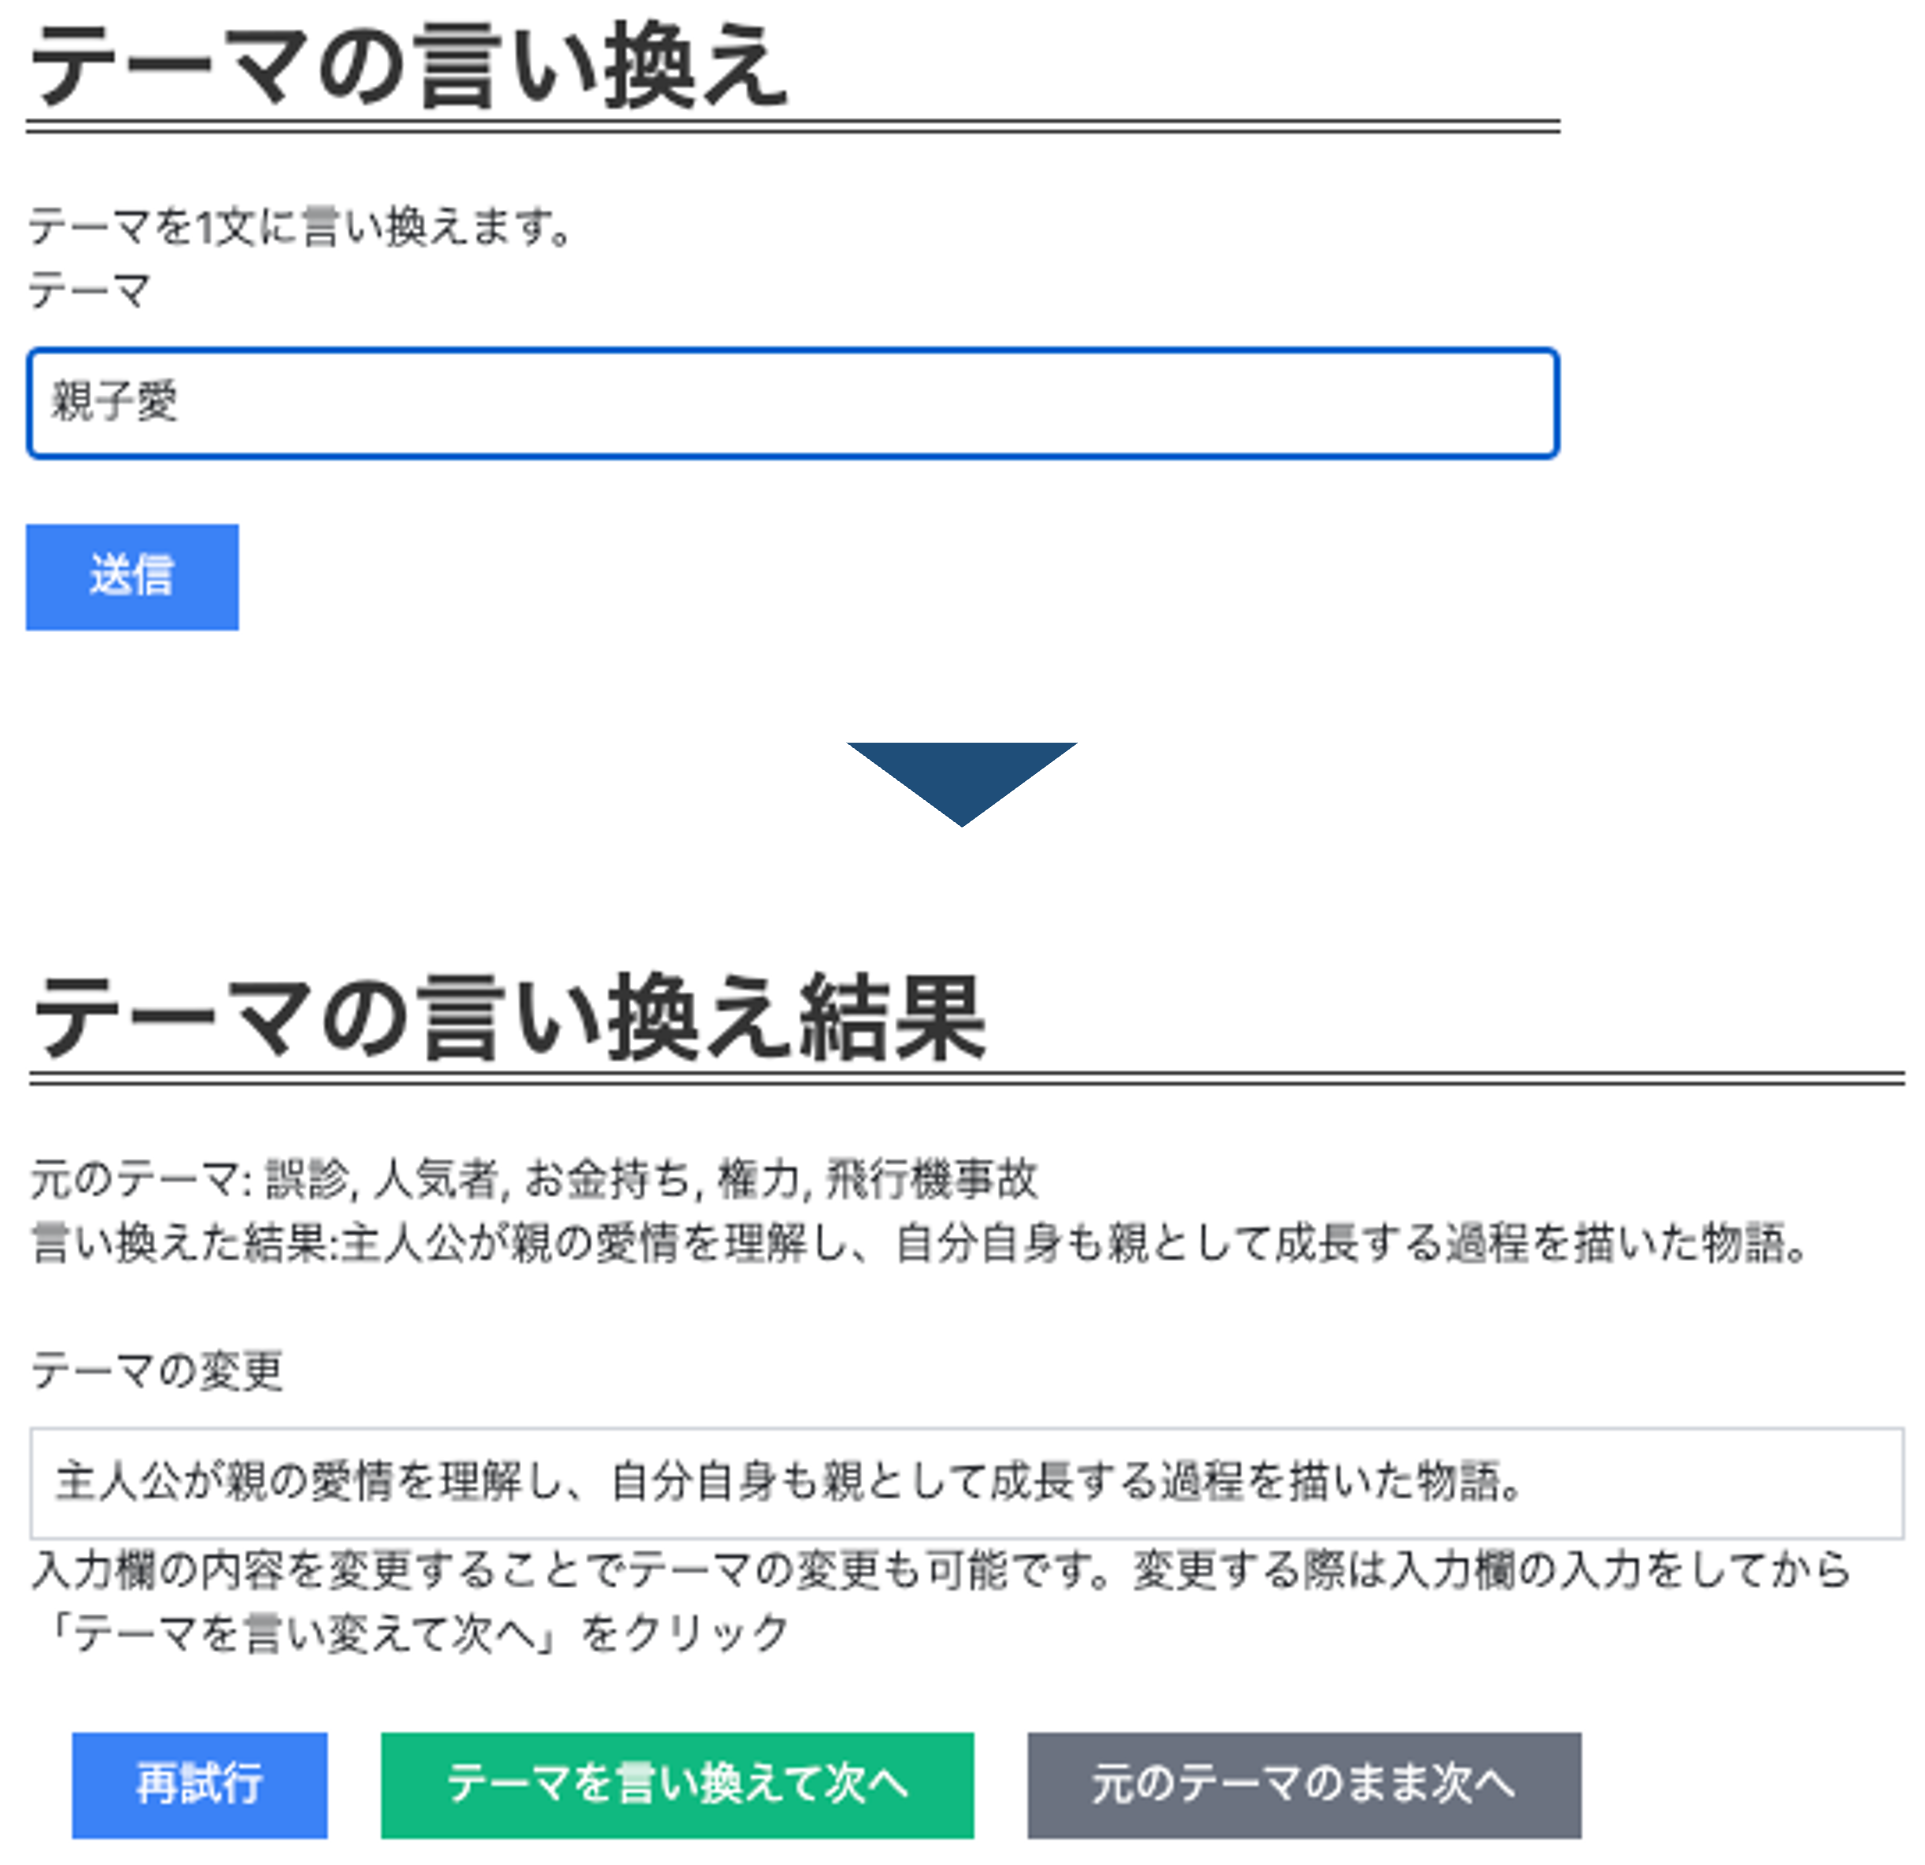
\includegraphics[width = 7cm]{pict/04/theme_change.png}
   \caption{テーマの言い換えを生成する画面の様子}
   \label{theme_change}
   \end{center}
\end{figure}

LLM は物語を生成する際, 入力として与えた単語をそのままの形で文章に登場させてしまう傾向がある. しかし, 物語のテーマは, 作品全体を通して伝わることが望ましく, 生成するプロットの中に直接単語として現れてしまうことは好ましくない.

テーマの言い換えの生成により, 文章形式でテーマを設定し直すことで, 選択したキーワードが生成するプロットの中に直接出てくることを防ぐことができる.

テーマの言い換えを生成する場合, ユーザーは図\ref{theme_change}の上部に示した画面上で, 言い換えたいテーマに関するキーワードをテキストエリアへ入力することを求められる. テキストエリアには, デフォルトで最初のステップにおいて選択したテーマや前のステップで生成した象徴表現となったテーマが入力されているため, 容易にキーワードを入力することができる. また, 自身で考えた言葉を入力し, その言い換えとなる文章を生成することもできる. その後,「送信」という青いボタンをクリックすることにより, 図\ref{theme_change}の下部に示した画面に遷移し, LLM を介して生成される, 入力したテーマに関するキーワードの言い換え表現を獲得することができる. 

生成されたテーマの言い換えは, デフォルトで図\ref{theme_change}下部に示した画面のテキストエリアへ入力され, 好ましい言い換えが生成された場合, 「テーマを言い換えて次へ」ボタンを押すことで, 生成されたテーマを言い換えた文章をプロットの設定へと反映させ, 次のステップへと移行することができる. 仮に気に入る言い換えが生成されなかった場合, 「再試行」ボタンをクリックすることで, 再度図\ref{theme_change}上部の画面に戻り, 新たな言い換えを生成することができる. また, 「元のテーマのまま次へ」ボタンを押すことにより, テーマの言い換えをせず次のステップへと移行することもできる. テーマの言い換えとして生成された文章は, ユーザー自身の手で書き換えることもできる.

テーマの言い換えの生成は, ストーリー生成におけるLLMの活用に有用であると同時に, ユーザーにテーマについて見直す機会を与えることも期待される. LLM からの生成を利用するだけでなく, ユーザー自身の手でテーマを言い換えることも可能である本システムは, ストーリークリエーターと LLM との共創を実現するものと考えられる.

\begin{center}
\begin{minipage}{0.7\textwidth}
\begin{itembox}[l]{テーマの言い換えの生成例}
\begin{center}
\begin{tabular}{cc} 
親子愛  →&\begin{tabular}{c}
親と子が互いの理解や共感を深め、\\困難を乗り越える過程を描く物語\end{tabular} 
\end{tabular}
\end{center}
\end{itembox}
\end{minipage}
\end{center}
\begingroup
\captionof{figure}{テーマの言い換えの生成例}
\label{theme_change_example}
\endgroup
\vspace{12pt}

\subsection{キャラクターの設定}
ここでは, 物語に登場させる, 『ブラック・ジャック』の既存キャラクターと, 自身で作り上げる新規キャラクターの設定を行うことができる. 図\ref{chara}で示したのは, 既存キャラクターの設定画面の様子である.

\begin{figure}[htbp]
   \begin{center}
   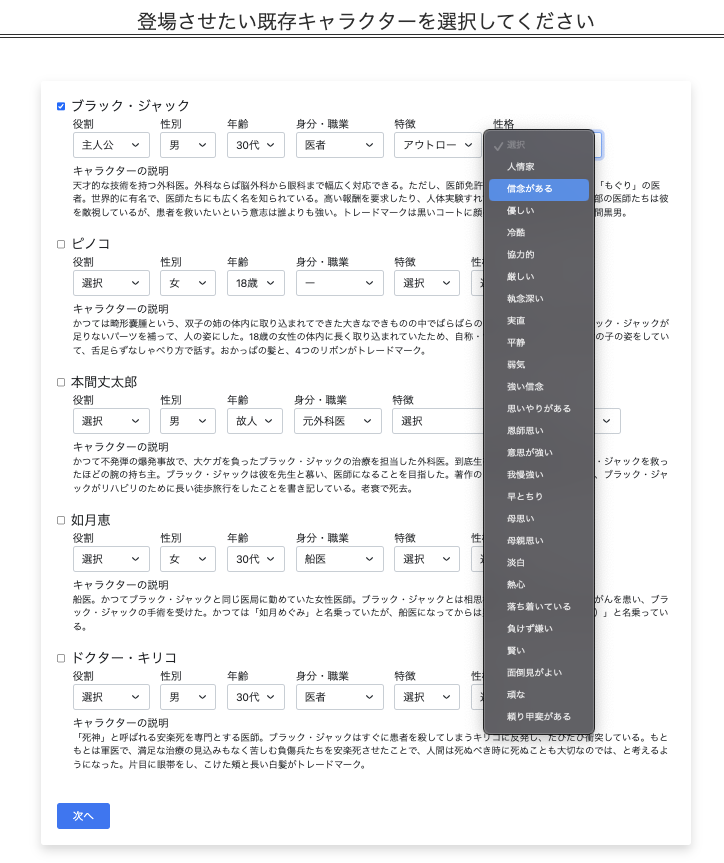
\includegraphics[width = 12cm]{pict/04/chara.png}
   \caption{既存キャラクターの設定画面.}
   \label{chara}
   \end{center}
\end{figure}

既存キャラクターには, 「ブラック・ジャック」や「ピノコ」など, 漫画『ブラック・ジャック』に登場する主要なキャラクターを選択肢として用意しており, ユーザーはその中からプロットに登場させるキャラクターを選ぶことができる. 図\ref{chara}に示したとおり, 既存キャラクターの設定は, キャラクター名の横のチェックボックスにチェックをいれ, 「役割」, 「性別」, 「年齢」, 「身分・職業」, 「特徴」, 「性格」の6つの属性を設定することで完了する. 6つの属性は, 『ブラック・ジャック』の物語構造分析に基づいた選択肢の中から選ぶことができ, 生成されるプロットにおいて, 既存キャラクターの言動が原作からかけ離れたものにならぬよう工夫を施している. 

それぞれのキャラクターの属性データは, 付録\ref{appendix:chara_attribute_list}に記す.

新規キャラクターの設定画面んを図\ref{newchara}に示す.

\begin{figure}[H]
   \begin{center}
   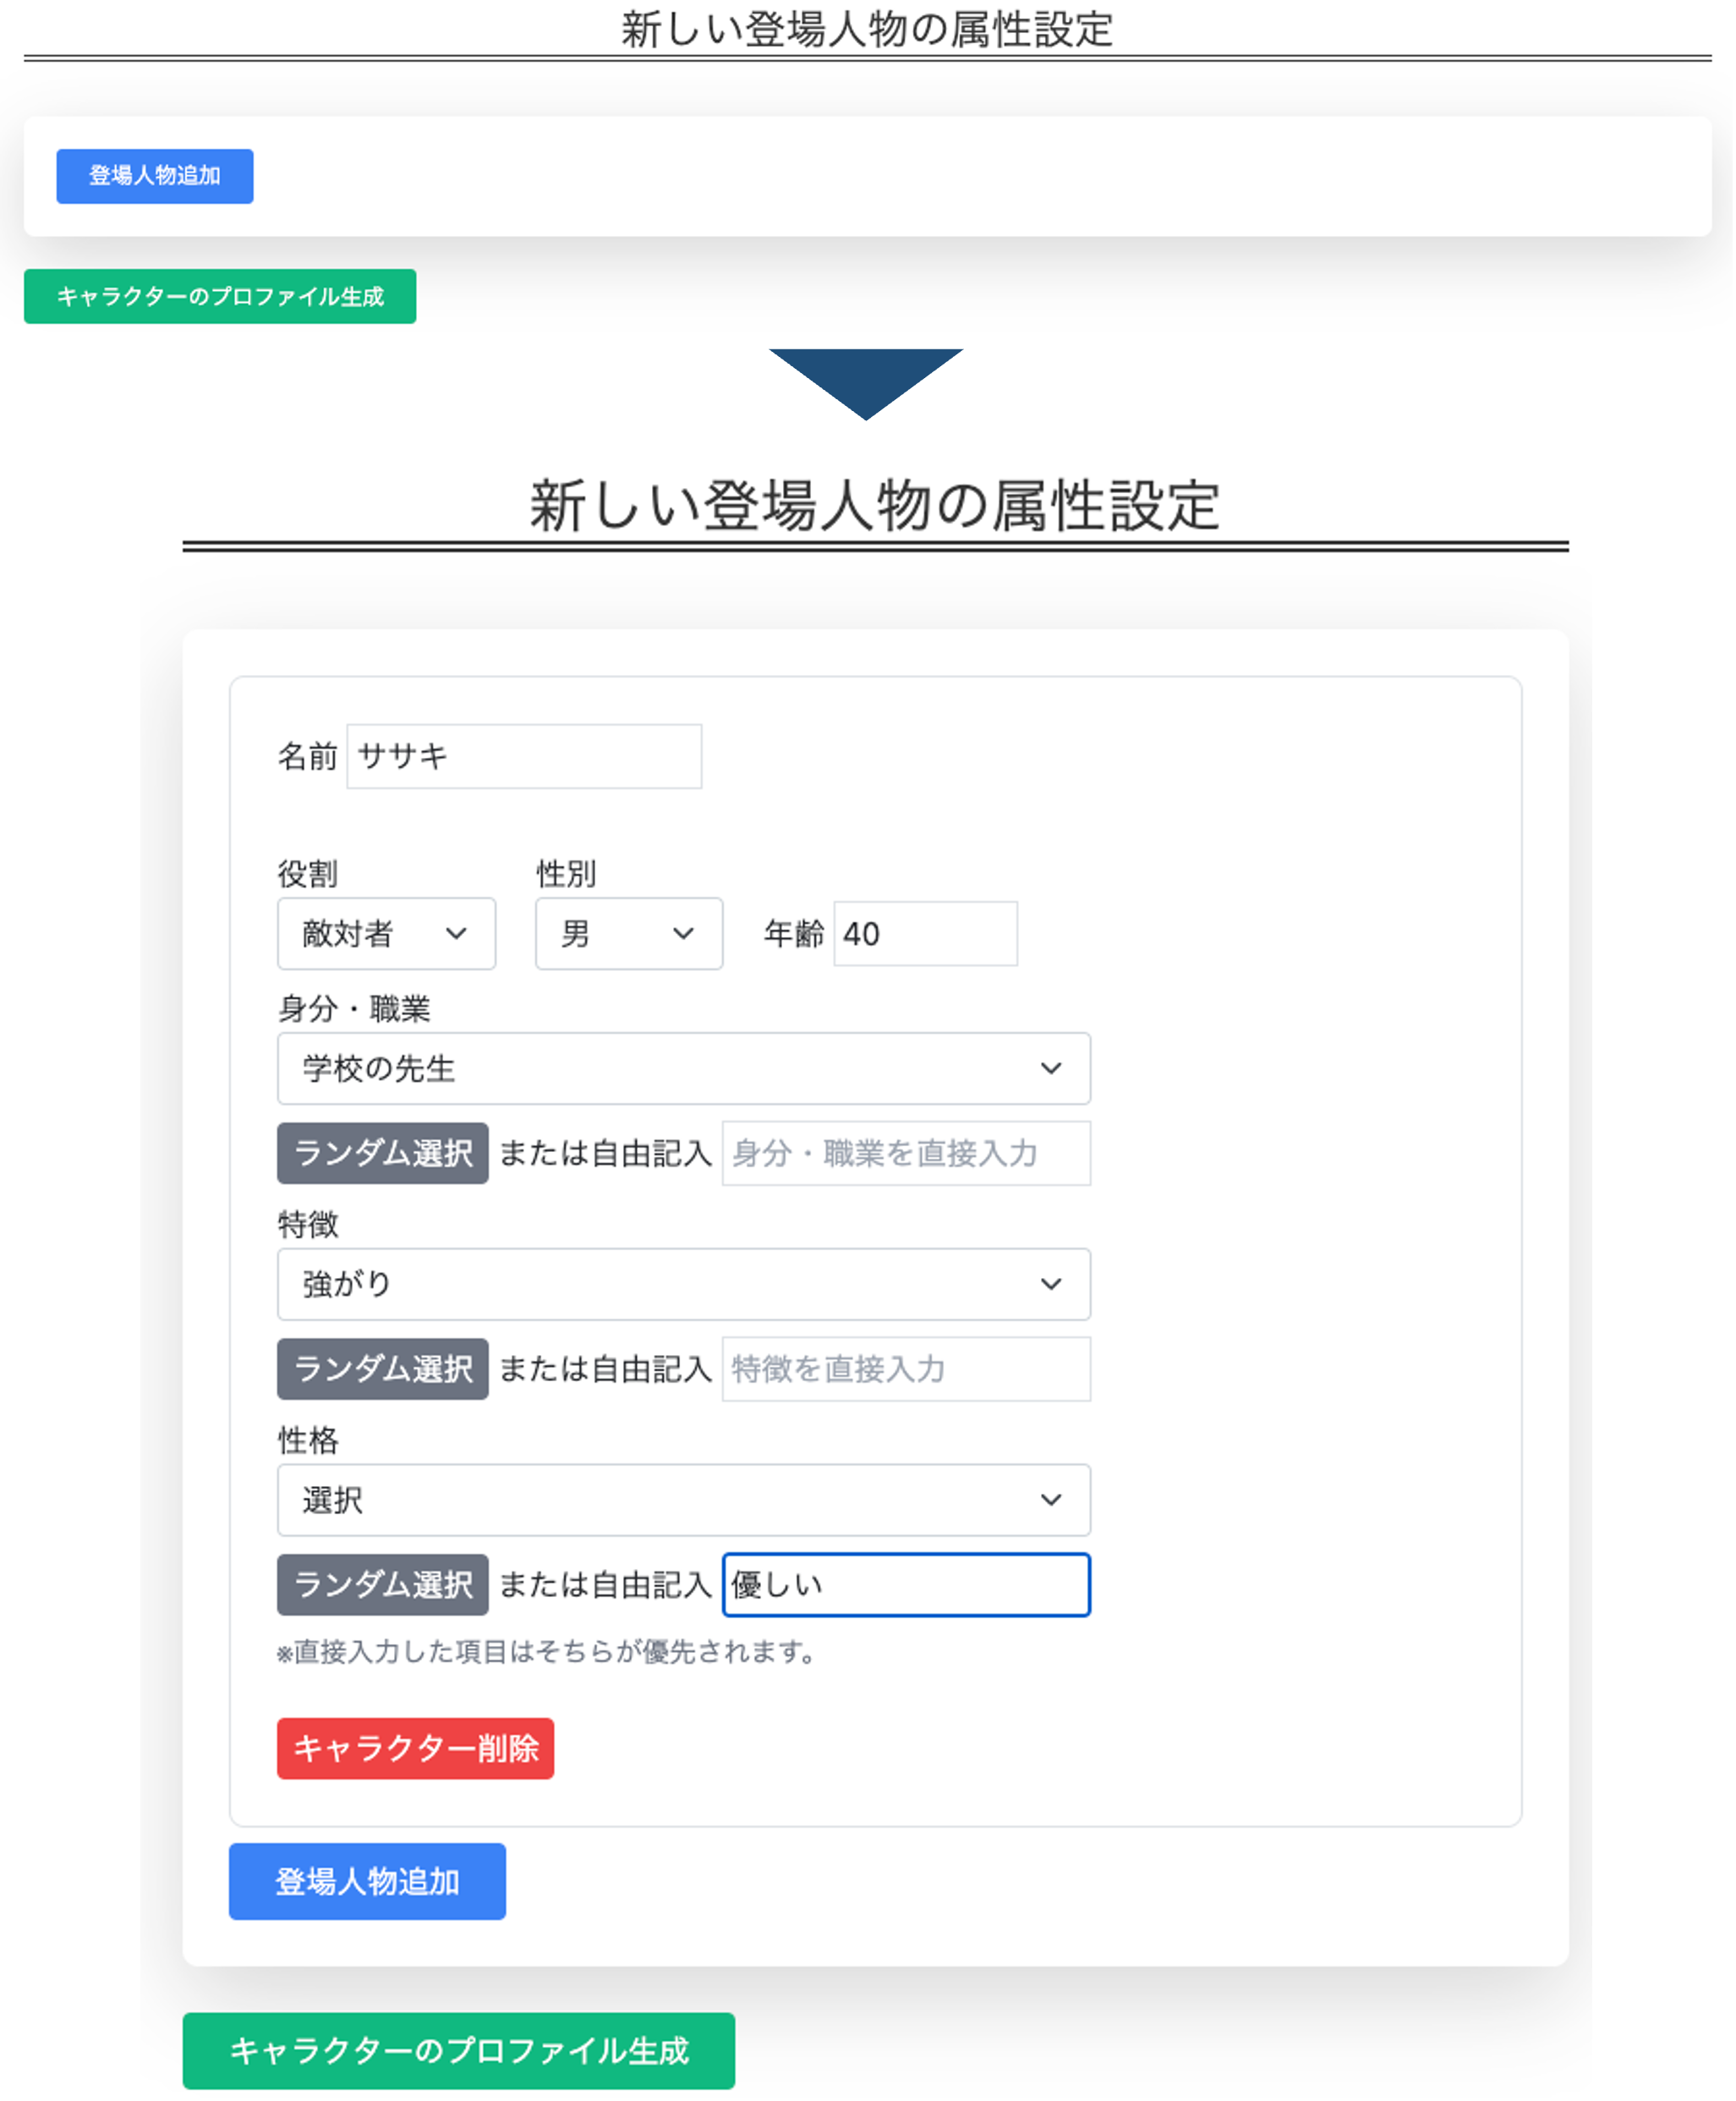
\includegraphics[width=10cm]{pict/04/newchara01.png}
   \caption{新規キャラクターの設定画面.}
   \label{newchara}
   \end{center}
\end{figure}

新規キャラクターの設定は, 「登場人物追加」という青いボタンをクリックすることで図\ref{newchara}の下部に示したようなコンテナが展開し, このコンテナ内で行うことができる. 新規キャラクターの属性として, 「名前」, 「役割」, 「性別」, 「年齢」, 「身分・職業」, 「特徴」, 「性格」という6つの属性を設定することができ, それぞれの項目について『ブラック・ジャック』のキャラクター分析に基づいた選択肢が用意されている. 用意された選択肢の中から属性を選ぶことも, ユーザー自身が思いついた言葉を当てはめることもでき, ストーリークリエーター自身のアイデアを尊重するとともに, 分析結果である選択肢の提示やランダム選択機能の提供により, 新規キャラクターの設定にかかる負担の軽減を図っている.

コンテナ内にある「登場人物追加」ボタンを押すことにより, また新たなキャラクターのためのコンテナが展開され, ユーザーはプロットに登場させたい人数分, 新規キャラクターの設定を行うことができる. 

登場させたい人数分, 新規キャラクターの属性を設定し終え, 「キャラクターのプロファイル生成」という緑色のボタンを押すと, 図\ref{newchara3}に示すように, それぞれのキャラクターに関するプロフィールを, LLM を介して生成することができる. 

\begin{figure}[hbtp]
   \begin{center}
   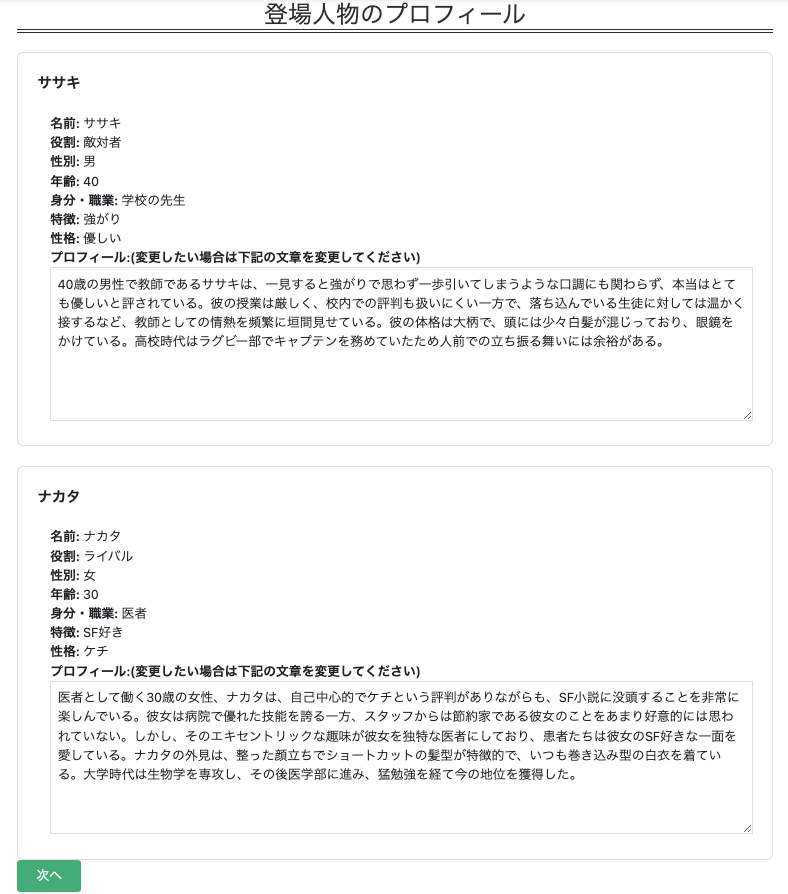
\includegraphics[width=10cm]{pict/04/newchara3.png}
   \caption{新規キャラクターのプロフィール生成画面.}
   \label{newchara3}
   \end{center}
\end{figure}

ここでいうプロフィールとは, キャラクターの背景や人物像をより詳細に説明する文章のことであり, これは作品上におけるキャラクターの言動に影響する\cite{mirowski23}. プロフィールは, 設定された属性をもとに生成され, その内容はユーザー自身の手で自由に書き換えることもできる. LLM とクリエーターとの共創を実現する.

生成されるプロフィールの例を図\ref{profile_example}に示す.

\begin{figure}[H]
   \begin{breakitembox}[l]{生成されるプロフィールの例}
      医者として働く30歳の女性、ナカタは、自己中心的でケチという評判がありながらも、SF小説に没頭することを非常に楽しんでいる。彼女は病院で優れた技能を誇る一方、スタッフからは節約家である彼女のことをあまり好意的には思われていない。しかし、そのエキセントリックな趣味が彼女を独特な医者にしており、患者たちは彼女のSF好きな一面を愛している。ナカタの外見は、整った顔立ちでショートカットの髪型が特徴的で、いつも巻き込み型の白衣を着ている。大学時代は生物学を専攻し、その後医学部に進み、猛勉強を経て今の地位を獲得した。
      \label{profile}
   \end{breakitembox}
\end{figure}
\vspace*{-1pt}
\begingroup
\captionof{figure}{生成されるプロフィールの例}
\label{profile_example}
\endgroup
\vspace{5pt}
キャラクターは物語に必要不可欠な要素であり, その設定は創作における重要な作業である. 本システムでは, 既存キャラクターと新規キャラクターの設定を, 『ブラック・ジャック』の物語構造分析に基づいた選択肢を用いて行うことができ, また, 新規キャラクターのプロフィール生成においては, LLMを活用し簡便な操作により行うができる. これらの機能は, ストーリークリエーターの創作支援に役立つものと考えられる.  

\subsection{物語展開因子と極性の設定}
物語展開因子とは, 物語の展開に影響を与えるとされる要素のこと\cite{murai21}である. 図\ref{factor}に物語展開因子の設定画面の一部を示す.

\begin{figure}[H]
   \begin{center}
   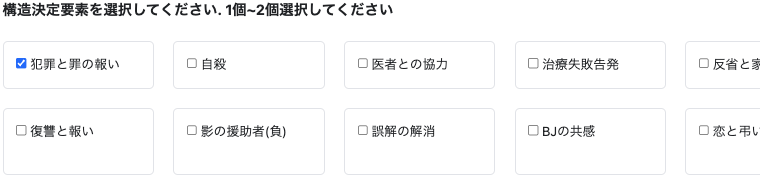
\includegraphics[width = 12cm]{pict/04/factor.png}
   \caption{物語展開因子の設定画面の一部.}
   \label{factor}
   \end{center}
\end{figure}

ここでは, 図\ref{factor}で示したように『ブラック・ジャック』の物語構造分析により得られた, 「犯罪と罪の報い」や「夫婦」など, 物語展開因子57種の中から, 物語に含めたい要素を複数選び設定することができる. 

ここで選択された物語展開因子をもとに, 次のステップにおいて設定される, 物語構造, 物語展開パターンの提案が行われる. つまり, ユーザーが物語に入れ込みたいと考えた因子により, その因子を含む物語として適う展開パターンが『ブラック・ジャック』の物語構造分析の結果に基づき得られることになるのである. 

物語構造, 物語展開パターンは, 物語の起伏, 流れを決定づける重要な要素であり, 本システムは, そのような要素を分析結果に基づき容易な操作によって利用することができるため, ストーリークリエーターの創作支援に役立つものと考えられる.

『ブラック・ジャック』の物語構造分析により得られた物語展開因子は以下の57種である.

\begin{breakitembox}[l]{物語展開因子一覧}
   BJの過去がテーマになっている話, ピノコに焦点が当たった話, キリコに焦点が当たった話, BJ目線での物語進行, 患者目線での物語進行, 妨害者目線での物語進行, 協力者目線での物語進行, 競合者目線での物語進行, 犯罪と罪の報い, 自殺, 医者との協力, 治療失敗告発, 反省と家族の支え, 医療勝負, 復讐と報い, 影の援助者(負), 誤解の解消, BJの共感, 恋と弔い(負), 記憶回復と家族復帰, 立場逆転からの償い, 男, 女, 乳幼児, 青少年, 大人, 老人, 親, 夫婦, 子, 家族親族, 恋人, 友人知人, 主人公, 味方, 敵, その他職業, 医療従事者, 店, 技術者, 運輸, 一次産業, 芸能, 軍事警察, 犯罪関係, 裁判関係, 教員, 魔術系, 客 患者も含まれる, 学生, 団体, 国家, 上級 金持ち、権力者等, 困窮者, 種族・人外, 動物, 死者
   \label{factor_list}
\end{breakitembox}

\begingroup
\captionof{figure}{物語展開因子一覧}
\label{factor_list_example}
\endgroup

また, このステップにおいては, 図\ref{polarity}に示したように, 物語の序盤, 終盤それぞれの場面における物語の極性を, -1(negative), 0(natural), 1(positive)の3つの数字の中から選び設定することができる.

\begin{figure}[H]
   \begin{center}
   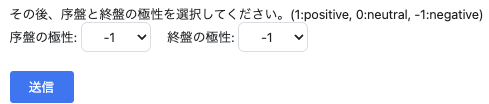
\includegraphics[width = 8cm]{pict/04/polarity.png}
   \caption{極性の設定画面.}
   \label{polarity}
   \end{center}
\end{figure}

物語の極性とは, 物語の各場面における雰囲気を表すものである. 例えば, 序盤に -1, 終盤に 1 を選ぶと, 物語は暗い雰囲気から始まり, 最後には明るい雰囲気で終わるようにすることができる.

ここで設定される極性も, 次のステップで行われる物語構造, 物語展開パターンの提案に用いられる. 極性の観点においてもユーザーの意向に適う, 物語構造, 物語展開パターンが, 物語構造分析の結果に基づき提案されることになる.

図\ref{polarity}に示した青い「送信」ボタンを押すことにより次のステップへと移行する.

\subsection{物語構造の設定}
ここでは, 『ブラック・ジャック』の物語構造, 物語展開が, 前のステップで選択された物語展開因子および極性に基づき, 4 から 11 の展開数ごとに複数提案され, ユーザーはその中から生成するプロットの物語構造を一つ設定することができる. これにより, ユーザー自身が含めたい要素に適う,『ブラック・ジャック』の分析に基づいた物語構造を生成するプロットの骨格として定めることができる.

例えば, 提案される物語構造には, 展開数5の場合, 「探索」→「依頼」→「看病・治療」→「情報開示」→「真相発覚」などがある.

生成される物語構造, 物語展開パターンの例を図\ref{structure}に示す.
\begin{figure}[H]
   \begin{center}
   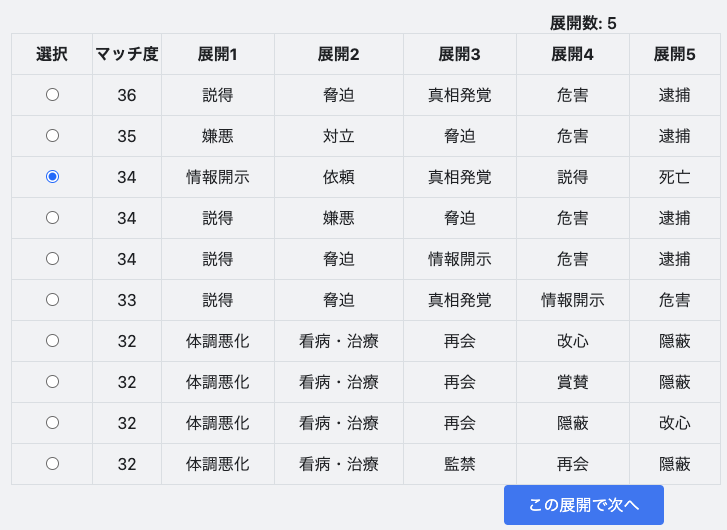
\includegraphics[width = 12cm]{pict/04/structure0.png}
   \caption{物語構造の設定画面の例.}
   \label{structure}
   \end{center}
\end{figure}

図\ref{structure}にあるマッチ度とは, ここで自動生成された物語構造, 物語展開パターンにおけるN-gramが, 先ほどのステップで選択された物語展開因子および極性に基づいて絞り込まれた既存の『ブラック・ジャック』のエピソードの物語構造, 物語展開パターンにおけるN-gramにどれだけ一致しているか, その出現頻度の合計として算出されるものである. したがってマッチ度は, その値が大きいほど, 生成された物語構造, 物語展開パターンが, 『ブラック・ジャック』の物語構造分析に基づく物語構造, 物語展開パターンに近いことを意味する.

マッチ度の計算を行うアルゴリズムを以下に示す.

\begin{algorithm}
   \caption{マッチ度の計算}
   \begin{algorithmic}[]
   \Require ユーザーに選定された物語展開因子 $f$
   \Require 『ブラック・ジャック』のエピソード群 $W$
   \Require 自動生成した物語展開パターン $P$
   \State 絞り込んだ対象エピソード群 $W'$ を計算: $W' = \{w \in W | w \text{ は因子 } f \text{ を含む}\}$
   \State 絞り込んだ対象エピソード群 $W'$ におけるN-gram集合 $N$ を計算
   \State 展開パターン $P$ 内に含まれるN-gram集合 $N_P$ を計算
   \State マッチ度 $M$ を計算: $M = \sum_{n \in N_P} \text{出現頻度}(n, N)$
   \Return マッチ度 $M$
   \end{algorithmic}
\end{algorithm}

マッチ度を参考に, 好みの物語構造, 物語展開パターンを選択し, 「この展開で次へ」のボタンを押すことにより, 選択した物語構造, 物語展開パターンをプロットの設定に反映させ次のステップへと移行することができる. 

本システムは, 物語構造分析の結果に基づく物語構造, 物語展開パターンの利用をこのような容易な操作により実現し, ストリークリエーターのストーリー創作を支援する.

\subsection{自由指示・時代・場所の設定および設定の確認編集}

ここでは, 物語の舞台となる時代や場所について設定することができ, また, これまで定めてきた設定を確認, 編集することができる. さらに, 自由記述による指示欄も設けており, 物語に含めたい要素を自由に設定することができる. 図\ref{settings0}に設定画面の様子を示す.

自由記述による指示は, プロットの設定を定めるこれまでの過程において受けた創造性への刺激を, ユーザー自身の言葉で表現する機会になると考える.

設定の確認や編集, 追記は, 図\ref{settings0}にしたような画面で行う. これまで設定されてきた内容がテキストエリアにデフォルトで入力されているため, それらの内容を単にテキストエリアへの入力という形で容易に確認, 編集することができる. また, ここで新たに行う, 時代や場所, 自由指示の設定においても同様で, テキストエリアへの入力により容易に行うことができる.

例えば, 図\ref{settings0}に示した画面では, 「時代」の設定が「現代」となっているが, これを「近未来」に変更することなどができる.

画面下部に, 「確認画面へ」という緑色のボタンがあり, そのボタンを押すと, 新たに書き換えた内容も含め確認する画面に遷移する. その画面下部にある「この設定であらすじを10種類生成(時間かかります)」という緑色のボタンを押すと, 確認された設定に基づき, 次のステップにおけるあらすじとタイトルの生成が行われる.

\begin{figure}[H]
   \begin{center}
   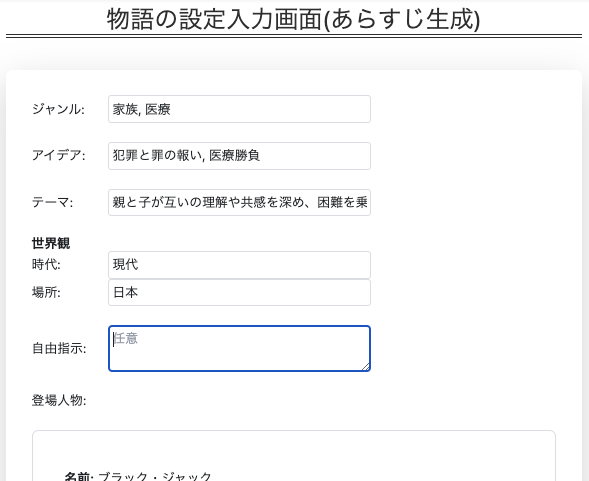
\includegraphics[width = 10cm]{pict/04/settings0.png}
   \caption{設定を確認編集する画面の様子}
   \label{settings0}
   \end{center}
\end{figure}

\subsection{タイトルとあらすじの生成}\label{self_method}
ここでは, これまで設定してきた情報をもとに, 1文から2文程度のあらすじとそれに付随するタイトルをそれぞれ10本生成することができる

なお, このステップは本システムの構築に際し筆者が行った提案のもと取り入れられた機能である. 筆者がこの機能の導入を提案した背景は次のとおり. 本システムが生成するプロットは漫画1話分のエピソードとして十分な量とするため, 1000字から1500字程度の長文である. したがって, 生成されるプロットについてその良し悪しを直感的に理解することは難しく, 生成にも時間がかかってしまう. そのため, イメージと異なるプロットの生成を何度も繰り返し行わせてしまうことはクリエーターの負担となってしまうと考えられた. この課題に対し, プロットの生成を前に, タイトルと1から2文程度のあらすじを生成させることを提案した. タイトルやあらすじは作品全体にまたがった影響を持つ重要な要素であり, そのイメージについて直感的な理解を与えるものである. タイトルとあらすじの生成をプロットの生成に先立って行うようにし, 長文であるプロットが生成される前に, あらすじやタイトルという直感的に理解できるもので, 作品全体の色を選択できるようにすることは, 出力されるプロットの制御性を高め, クリエーターの負担を軽減すると考えられる. また, タイトルやあらすじは, クリエーターの作品全体に対する枠組みや指針へのイメージの具体化に役立ち, それ自体が創造性への刺激としても役立つと考えられる.

図\ref{synopsis}に生成されたタイトルおよびあらすじの確認および設定画面の様子を示す. 図\ref{synopsis_example}に, 生成されるタイトルおよびあらすじの例を示す.

\begin{figure}[H]
   \begin{center}
   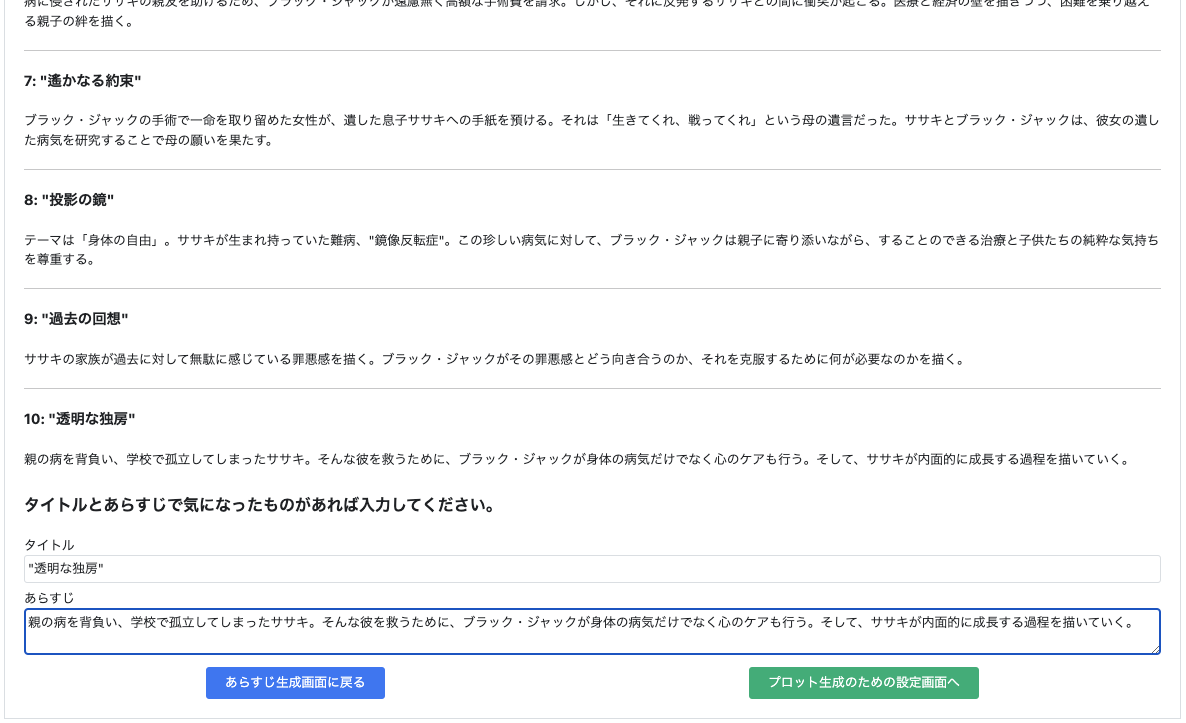
\includegraphics[width = 12cm]{pict/04/synopsis.png}
   \caption{生成されたタイトルおよびあらすじの確認および設定画面の様子}
   \label{synopsis}
   \end{center}
\end{figure}

\begin{breakitembox}
   [l]{タイトルとあらすじの生成例}
   \noindent タイトル: 透明な独房 \\
   あらすじ: 親の病を背負い、学校で孤立してしまったササキ。そんな彼を救うために、ブラック・ジャックが身体の病気だけでなく心のケアも行う。そして、ササキが内面的に成長する過程を描いていく。
\end{breakitembox}
\vspace*{-5pt}
\begingroup
\captionof{figure}{タイトルとあらすじの生成例}
\label{synopsis_example}
\endgroup
\vspace{5pt}

ここで生成されたタイトルおよびあらすじは, 図\ref{synopsis}に示した画面下部にあるタイトル, あらすじのテキストエリア内に入力することにより, その内容をプロットに反映させることができる. このテキストエリア内でタイトルやあらすじを修正することもでき, ストーリークリエーターと LLM との共創を実現する. 

画面下部にある「あらすじ生成画面に戻る」を押せば, 再度設定を見直し, タイトルおよびあらすじの生成を行うことができ, 「プロット生成のための設定画面へ」を押すことで次のステップへと移行することができる.

\subsection{アイデアの生成}
ここでは, これまでの設定をもとに, 具体的な出来事や道具など, プロットの中で用いることができそうな物語全般に関するアイデアを生成することができる. 生成されたアイデアは, これまでの情報をプロットにまで拡張する材料になり得ると考える. 

図\ref{idea}は, アイデアが生成された画面を示している. 物語に用いたいと思うアイデアが生成された場合, 画面下部にある, アイデアのテキストエリア内に, そのアイデアを入力することにより, その内容をプロットに反映させることができる. このテキストエリア内でアイデアを修正することも, ユーザー自身で考えたアイデアを入力することも可能で, ストーリークリエーターと LLM との共創を実現する.

画面下部にある「アイデア生成画面に戻る」を押せば, 再度設定を見直し, アイデアの生成を行うことができ, 「プロット生成のための設定画面へ」を押すことで次のステップへと移行することができる.


\begin{figure}[H]
   \begin{center}
   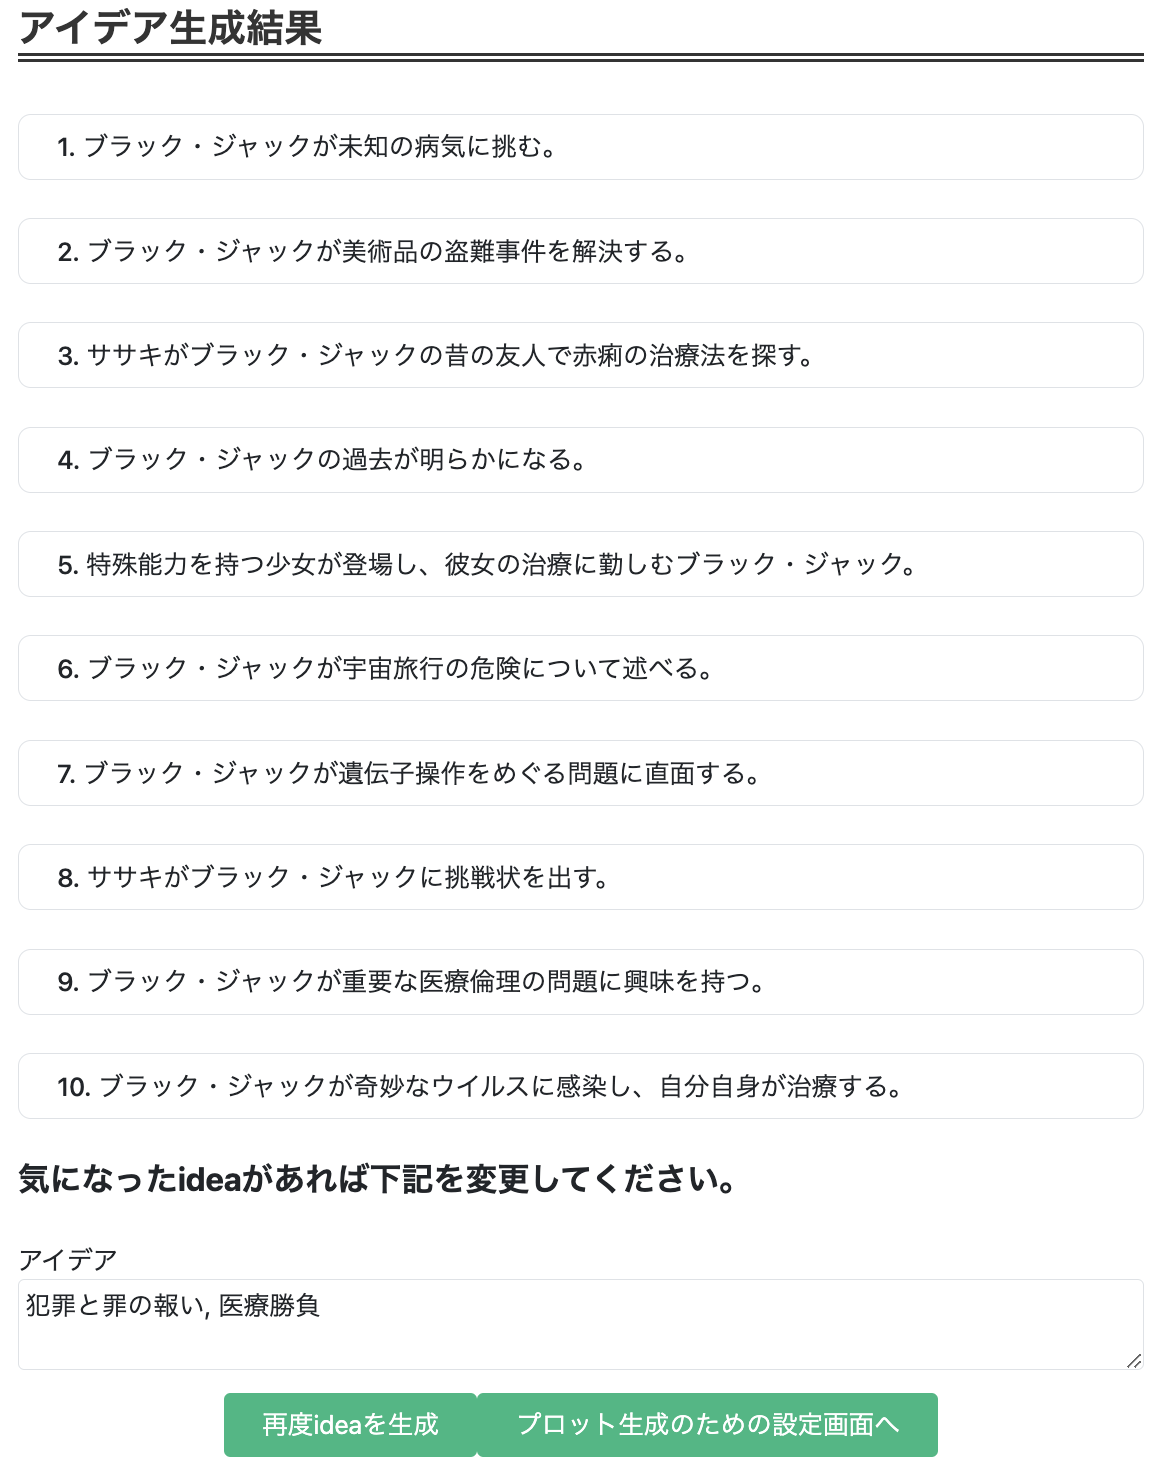
\includegraphics[width = 7.5cm]{pict/04/ideas.png}
   \caption{生成されたアイデアの確認および設定画面の様子}
   \label{idea}
   \end{center}
\end{figure}


\vspace{5pt}

図\ref{idea_example}に, 生成されるアイデアの例を示す.

\begin{center}
\begin{minipage}{0.7\textwidth}
\begin{itembox}[l]{アイデアの生成例}
   \begin{center}
   失われた古代医学の再発見
   \end{center}
\end{itembox}
\end{minipage}
\end{center}
\vspace*{-8pt}
\begingroup
\captionof{figure}{アイデアの生成例}
\label{idea_example}
\endgroup

\subsection{シーンごとの主観視点等最終設定およびプロットの生成}
ここでは, プロットの各シーンを誰の視点で描くか設定するとともに, これまで定めてきた設定を確認, 修正することができる. 図\ref{settings}は, これまでの設定を確認修正している画面の様子である. これまで定めてきた設定が, テキストエリアの中にデフォルトで入力された状態になっており, 確認, 修正は容易に行うことができる.

\begin{figure}[H]
   \begin{center}
   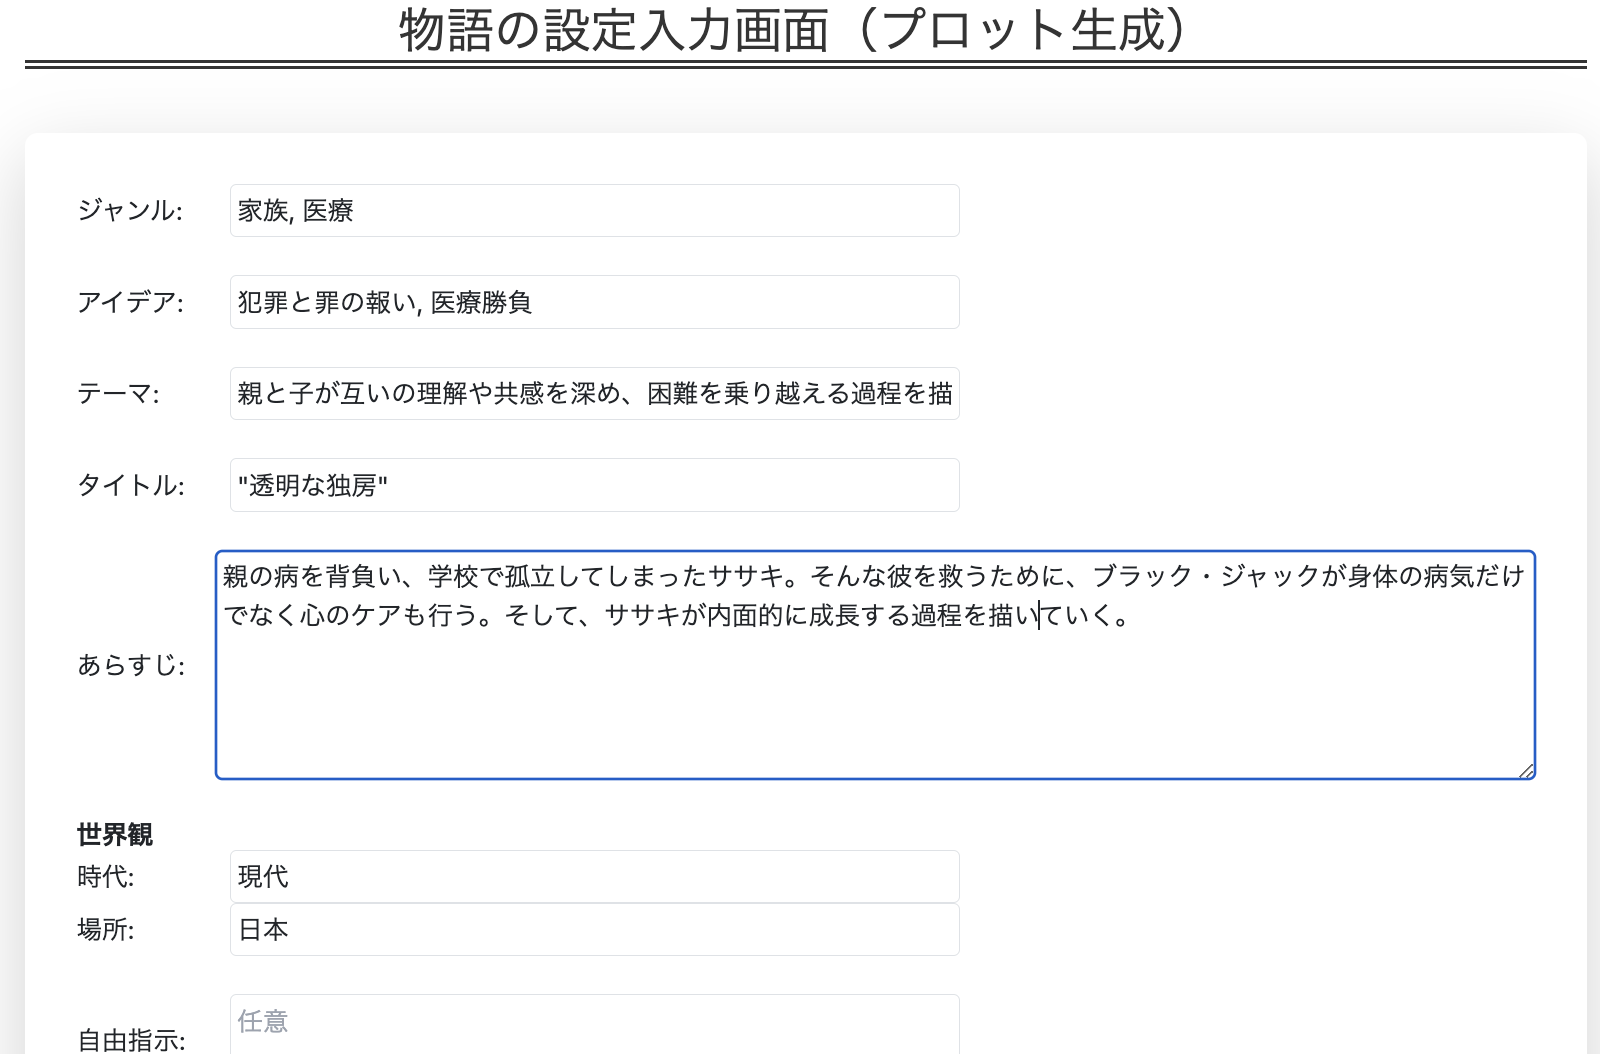
\includegraphics[width=13cm]{pict/04/finalsettings.png}
   \caption{設定の最終確認画面}
   \label{settings}
   \end{center}
\end{figure}

このステップでは, これまでの設定を整理するとともに, これまでの作業を通じて想起された新たなアイデアを盛り込む機会となり, ストーリークリエーターの創作支援に役立つものと考えられる. 図\ref{settings}で示した画面を下にスクロールしていくと, 図\ref{perspective}で示したテキストエリアが現れる. 各テキストエリア内にキャラクター名を入力することで, 生成されるプロットにおいて, それぞれのシーンを指定したキャラクターの視点で描かせるよう指示を与えることができる.

\begin{figure}[H]
   \begin{center}
   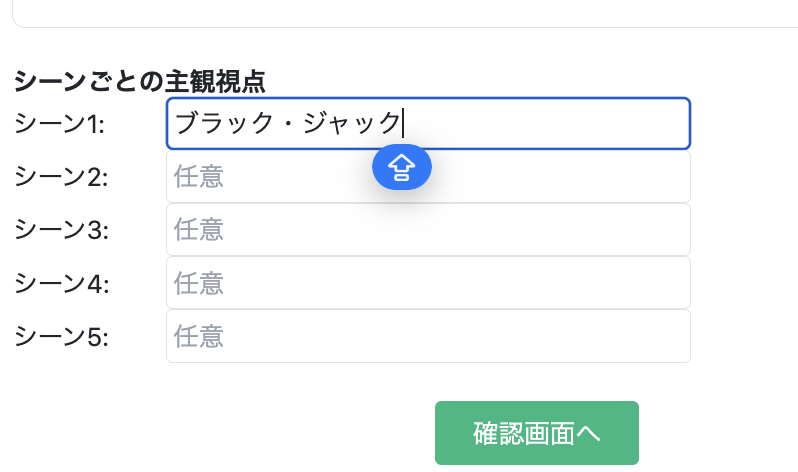
\includegraphics[width=7cm]{pict/04/perspective.png}
   \caption{シーンごとの主観視点の設定画面}
   \label{perspective}
   \end{center}
\end{figure} 

シーンごとに主観視点を決められるこの機能は, 本システムの制作段階で, クリエーターから頂いた意見をもとに実装した機能であり, シーンごとに視点を変えることで, 物語に複雑性を持たせられるようにする狙いがある.

テキストエリアにはデフォルトで「任意」の文字が入力されており, 指定しなければ, そのシーンは任意の視点で描かれることになる.

ここでの確認, 修正がプロット生成を行う前の最終段階であり, 全ての設定を確認し終え, 図\ref{perspective}「確認画面へ」を押すとこれまでの設定, 修正を確認するページへと遷移し, そのページにおいて「この設定でプロットを生成」ボタンを押すことにより, これまでの設定を反映させたプロットを生成することができる. 図\ref{plot_example}に生成されるプロットの例を示す.


\vspace{10pt}
\begin{breakitembox}
   [l]{プロットの生成例}
   \noindent{シーン1: 依頼}\\
1. 夜明け前、ササキと名乗る男がブラックジャックの診療所にやってくる。彼は昔の友人であり、現在は小学校の校長だった。\\
2. 戸惑いを見せる彼にブラックジャックは、とりあえず部屋に招き入れ、事情を話すよう促す。\\
3. ササキは自身が命に関わる病に冒されており、それを理由に学校の生徒たちから非難を浴び、心底孤立してしまったと言う。\\
4. ササキは詐病だと疑われ、周囲からは見放されたと悔しそうに告白する。\\
5. `それでは色々調査してみましょう、もしご相談があれば何でもお伝えください。'とブラックジャックは静かに答えた。\\
\\
{シーン2: 看病・治療}\\
1. 検査の結果、ササキの病気は一般医学では治療困難な珍しい病で、ブラックジャックだけが治療法を知っていた。\\
2. 著しい無力感と医師の傲慢さに直面し、ブラックジャックは患者の感情的な側面と向き合い、彼を助けようと決意する。\\
3. ブラックジャックとピノコは、彼の家族や生徒たちがササキと連絡をとりたがらないことを知り、これが学校の中の性差別問題だと理解した。\\
4. ブラックジャックはリハビリをササキに行い、合わせて心のケアも施し始めた。\\
5. ササキの心のケアは、彼が自身に自信を持つように導くためでもあった。\\
\\
{シーン3: 危機}\\
1. 看病が進む中、突如としてササキの身体に危機が迫った。\\
2. ブラックジャックはササキを急遽手術台に乗せ、彼の命を救うための全力を尽くした。\\
3. しかし、手術の最中に突然電源が落ち、全ての機器が停止した。\\
4. 手術は延長され、ササキの命は一時的に揺らいだ。\\
5. 突然の事態に院内はパニックになり、ブラックジャックは事の解決に奔走した。\\
\\
{シーン4: 依頼}\\
1. 電源が落ちたのは病院の裏切り者による仕業だと判明。\\
2. 裏切り者はササキを助けるために金を渡すようブラックジャックに要求した。\\
3. しかし、ブラックジャックがその要求には応じず、ササキを助けることに全力を尽くした。\\
4. 電源は元に戻り、ササキの手術は無事終了、ササキは一命を取り留める。\\
5. ササキの元生徒たちが次々と病室を訪ね、彼との和解を選び始める。\\
\\
{シーン5: 嫌悪}\\
1. 再び訪れた夜明け、ササキは自身の中に変化を感じ、ブラックジャックに感謝を伝えた。\\
2. ササキは学校に戻り、生徒たちに対して自分が病気であることを公に告白した。\\
3. それはササキの成長を示した瞬間であり、ブラックジャックは嬉しく思った。\\
4. しかし、ササキはまた孤立してしまうのではないかという不安も抱いていた。\\
5. '人は孤独だ、だからこそ助け合い、理解し合うことが大切だ。'とブラックジャックはササキに言い、彼に自身の孤独と向き合う勇気を与えた。\\
\end{breakitembox}
\vspace*{-5pt}
\begingroup
\captionof{figure}{プロットの生成例}
\label{plot_example}
\endgroup


生成されたプロットは, 図\ref{plot}のように表示される.
\begin{figure}[H]
   \begin{center}
   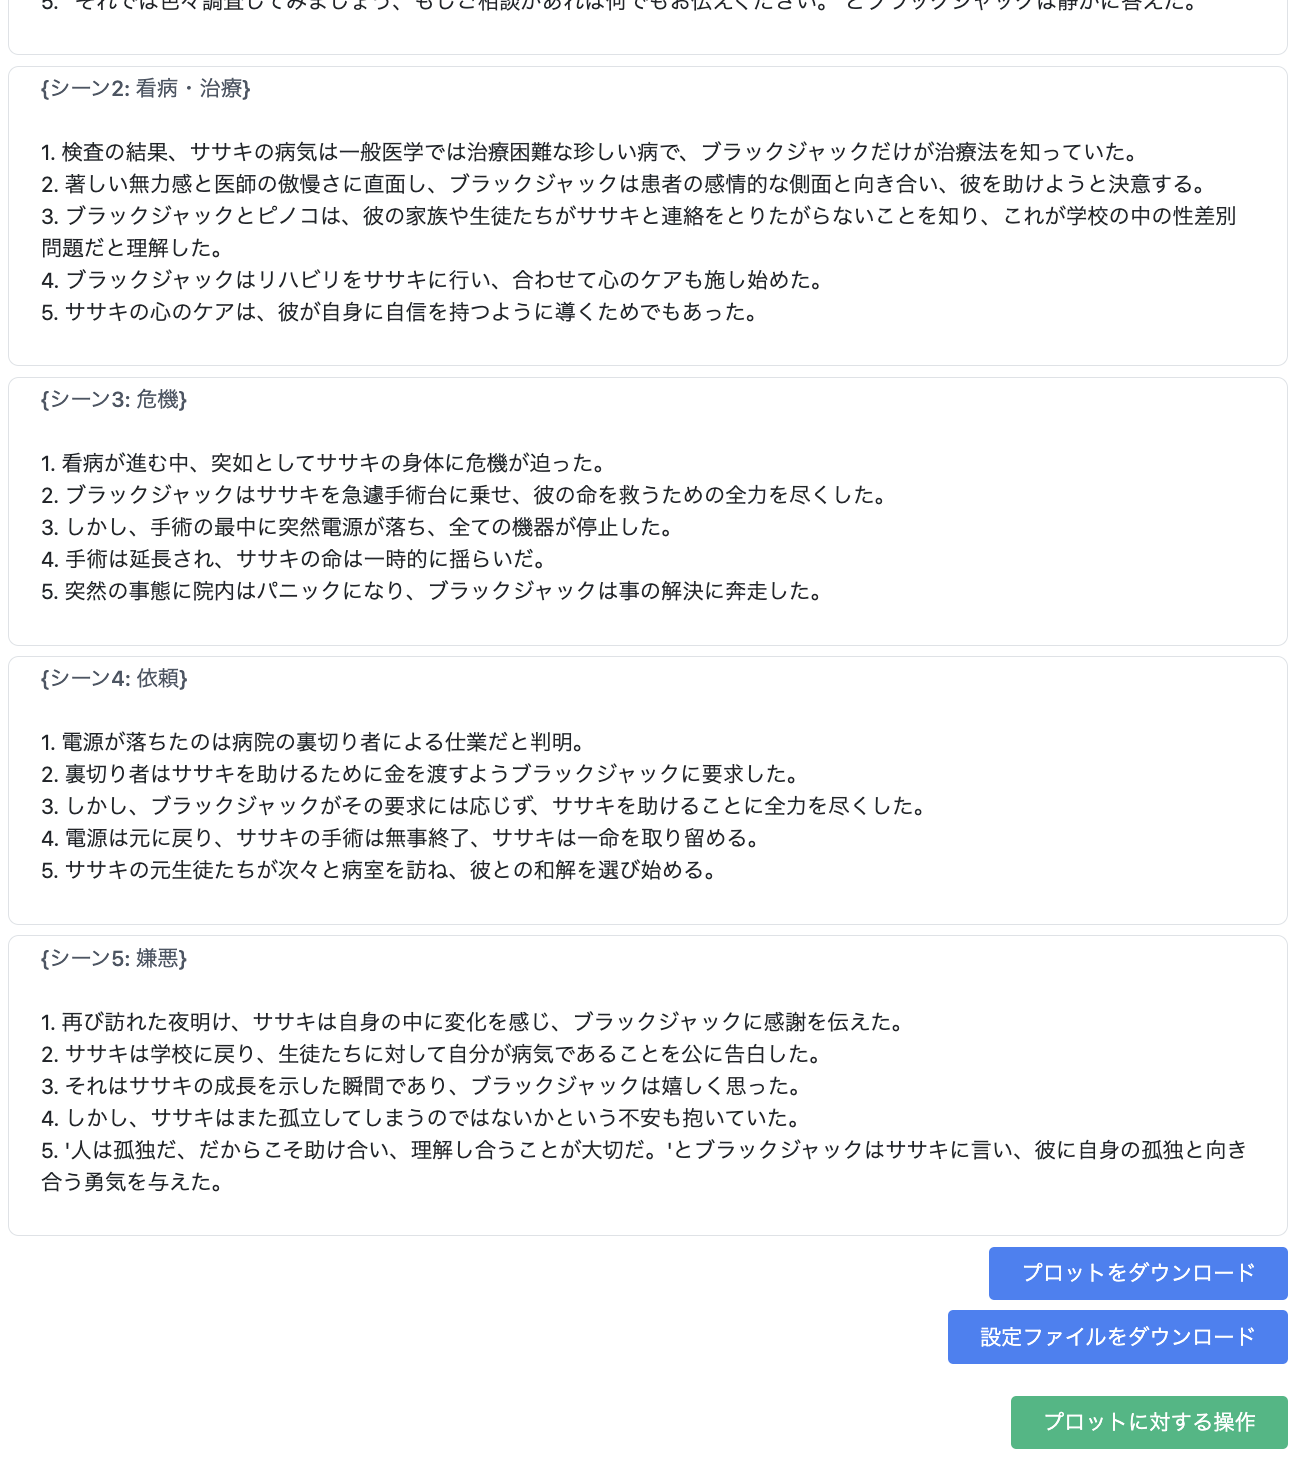
\includegraphics[width=10cm]{pict/04/plot.png}
   \caption{生成されたプロットの確認画面の様子}
   \label{plot}
   \end{center}
\end{figure}

画面下部にある「プロットをダウンロード」のボタンを押すことで, プロットをテキストファイルとしてダウンロードすることができる. また, 画面下部にある「設定ファイルをダウンロード」を押すことで, これまでの設定を記録した設定ファイルをダウンロードすることができ, 下部にある「プロットに対する操作」ボタンを押すことにより, プロット編集セクションへと遷移することができる.

プロット生成セクションでは, 上記のように, 物語構造分析に基づくLLMを活用したプロット生成を, 簡便な操作により実現し, ストーリークリエーターとLLMとの共創手法を提供することで, ストーリークリエーターの創作を支援する.

\section{プロット編集セクション}\label{sec:plot_edit}
本システムにおいては, プロットを生成する機能だけでなく, LLMとのインタラクティブなやり取りによりプロットを反復的に洗練させていくことができるプロット編集セクションを実装した. これは, LLMの活用において, 単に一度プロットを生成させるだけでは満足のいくプロットを得ることが難しいという問題と, LLMとのインタラクティブなやり取りそのものが創造性の拡張に期待されるという考えに基づくものである. LLMの利点において,体力的制約を持たないという利点と即時応答という利点が挙げられるが, この機能はこれらの利点を活かす機能となっている.

このセクションでは, 既存のプロットを, LLMを介し新たな指示や要素を加えて書き換えることができる. 新旧プロットを比較し, 満足のいくプロットを採用していく反復的な過程を通じてプロットの質を高めることができ, この機能によりクリエーターと LLM とのプロット生成における共創を実現する. そのフローは下図\ref{flow2}の青枠で囲われた部分のようになっている. 

示したフローのように, 既存のプロットに対する編集機能の適用と, 書き換えられた新たなプロットと既存のプロットとの比較を反復的に行うことで, プロットを満足のいく形へと変化させることができる. その過程において提供される LLM とのインタラクティブ手法を通じた共創の実現により, ストーリークリエーターの創作を支援する.

\begin{figure}[H]
   \begin{center}
   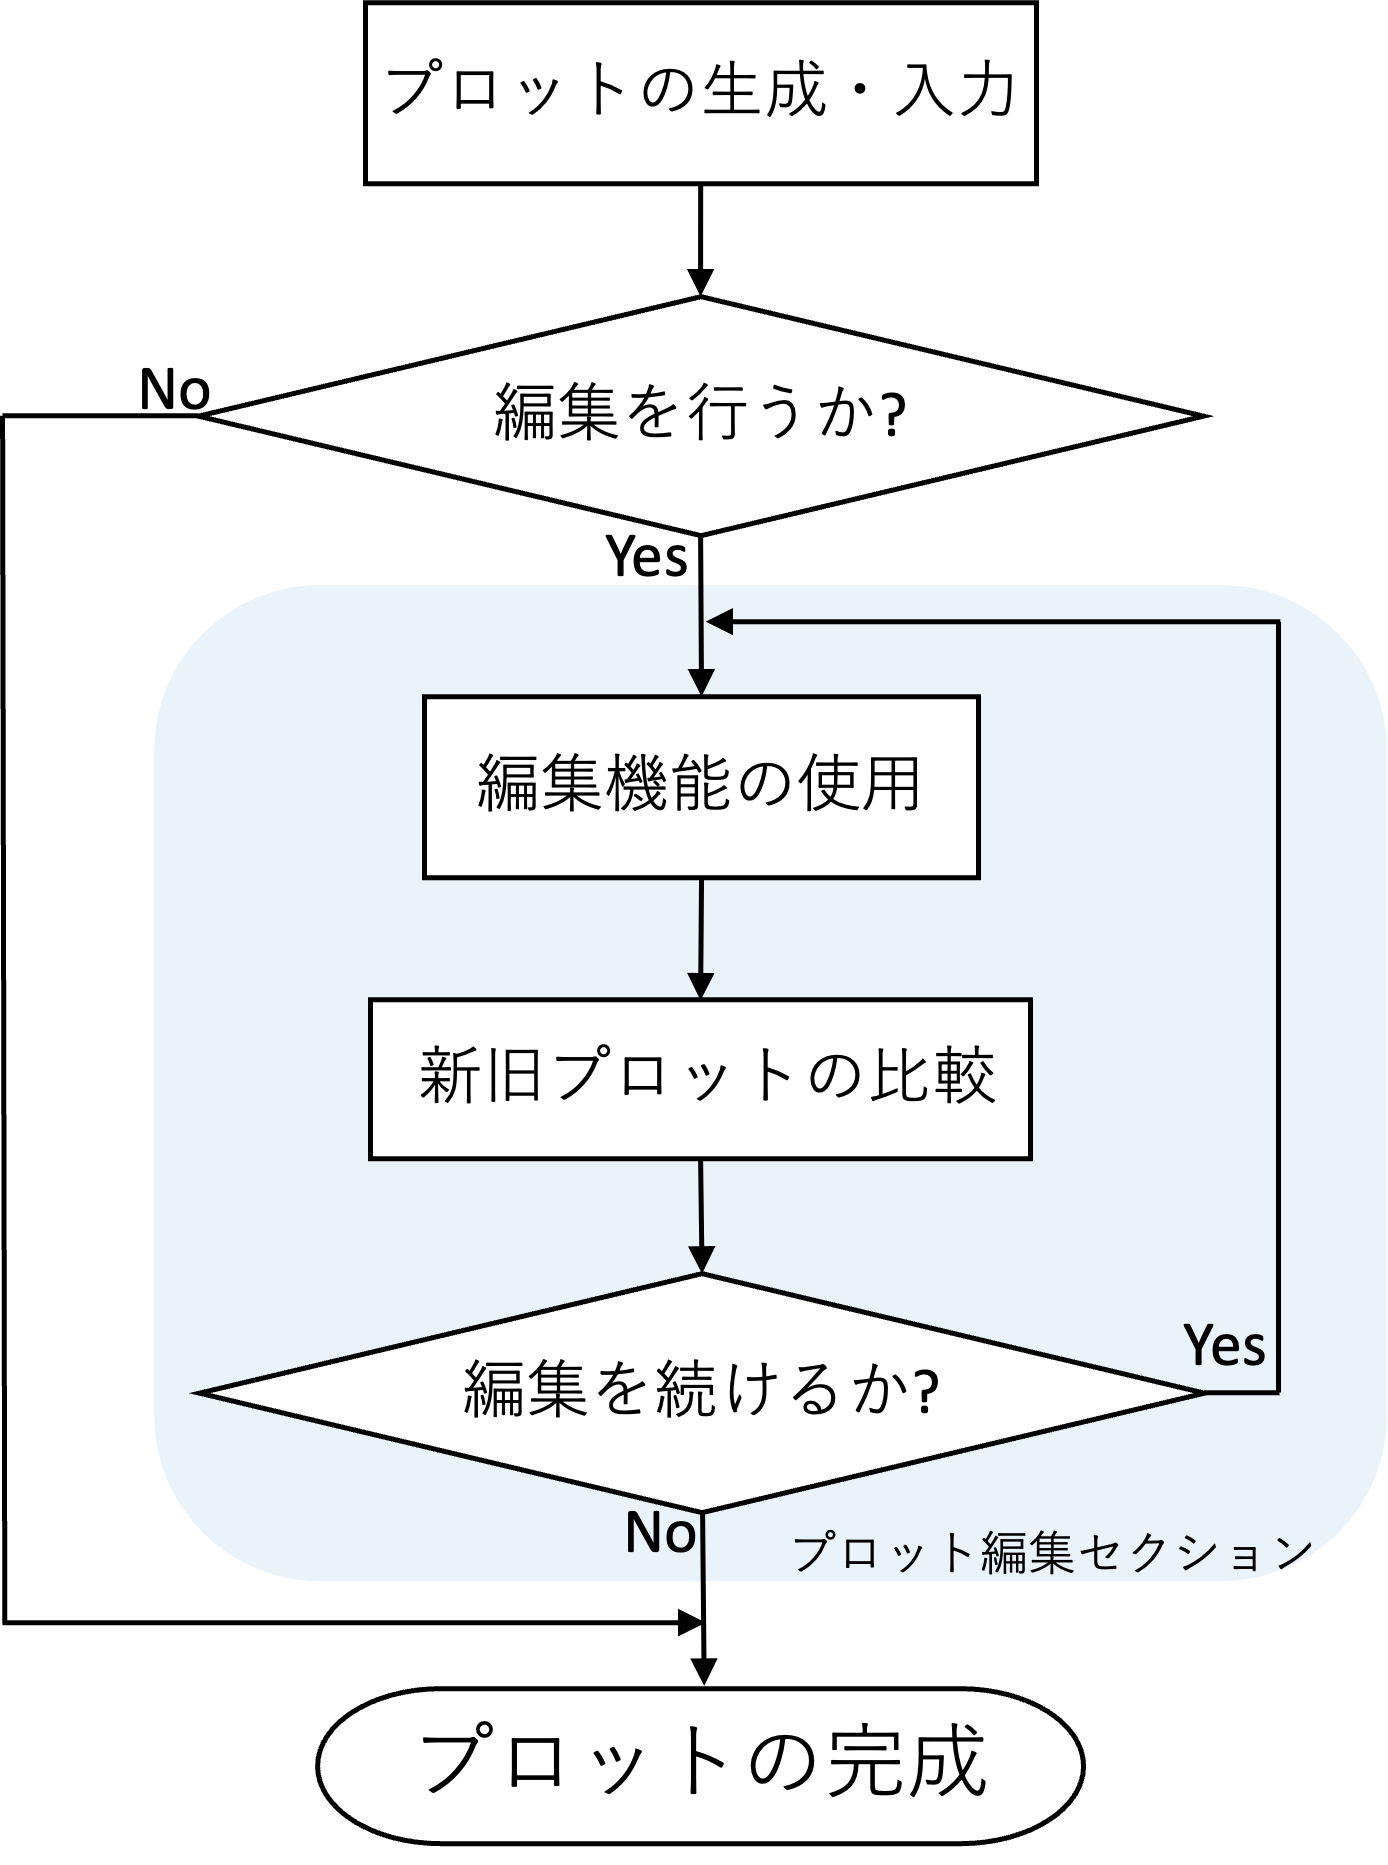
\includegraphics[width=6cm]{pict/04/flow2.png}
   \caption{プロット編集セクションにおけるフロー.}
   \label{flow2}
   \end{center}
\end{figure}

実装したプロット編集機能の一覧を以下に示す.
\begin{itemize}
\item \hyperref[subsec: freeword]{フリーワードによるやり取り}
\item \hyperref[subsec: question]{プロット中の単語・文章に関する質問}
\item \hyperref[subsec: idea]{アイデア生成}
\item \hyperref[subsec: foreshadowing]{伏線の処理}
\item \hyperref[subsec: change]{一部シーン変更}
\item \hyperref[subsec: atmosphere]{全体的な雰囲気の変更}
\item \hyperref[subsec: swap]{シーンの入れ替え}
\item \hyperref[subsec: perspective]{シーンごとの視点の変更}
\item \hyperref[subsec: add]{登場人物の追加}
\item \hyperref[subsec: change_role]{登場人物の役割変更}
\item \hyperref[subsec: modify]{プロットの部分修正}
\item \hyperref[subsec: modify_japanese]{不自然な日本語の修正}
\item \hyperref[subsec: divide]{プロット1シーンの起承転結への分割}
\item \hyperref[subsec: manual]{手作業での編集}
\end{itemize}

以下ではまず, これらの機能の適用後に遷移する新旧プロットの比較画面について説明し, その後, この一覧に示した機能について順に説明する.

\subsection{新旧プロットの比較}\label{subsec: comparison}
図\ref{flow2}のフローで示した通り, プロット編集セクションでは, 編集機能を適用して既存のプロットを新たなプロットへと書き換えると, 既存のプロットとそれを書き換えた新たなプロットとを比較する画面に遷移する. この画面では, 新旧プロットが左右に表示され, 2つのプロットを比較することができ, 新旧のプロットを比較した結果として, 既存のプロットを採用するか, 新しいプロットを採用するか, 2つのプロットを手作業で統合するかを選ぶことができる. 

このように, プロット編集セクションでは, ユーザー自身の判断によりプロットをより満足のいく形へと改善していくことができ, これは, ストーリークリエーターにとり LLM の効果的なインタラクティブ手法になると考えられる.

新旧プロットを比較する画面の様子を図\ref{comparison}に示す. 図\ref{comparison}の左下部に示されている, 灰色の「採用せず元に戻る」のボタンをクリックすると, 新たに生成されたプロットを破棄して, 各々の編集機能の画面へ戻ることができる. その右隣りにある赤い「採用せず次に進む」のボタンをクリックすると, 既存のプロットを採用し, 編集を続けるか否かを判断するページへと遷移することができる. その右隣りにある緑色の「手動で双方を混合」のボタンをクリックすると, 2つのプロットを手作業で統合するための画面へと遷移し, 2つのプロットを手作業で統合することができる. 図\ref{flow2}の右下部にある, 青色の「採用して次に進む」のボタンをクリックすると, 新たに生成されたプロットを採用し, 編集を続けるか否かを判断するページへと遷移することができる. さらに, 図\ref{flow2}の右側に示されている新しいプロットの下に付されている「ダウンロード」ボタンをクリックすると, 新たに生成されたプロットをテキストファイルとして保存することができる.

手作業で2つのプロットを統合する際は, 生成されたプロットを受けて想起された新たなアイデアを盛り込む機会にもなる.

このような機能を通じて, ストーリークリエーターと LLM との共創を実現し, ストーリークリエーターの創作を支援する.

\begin{figure}[H]
   \begin{center}
   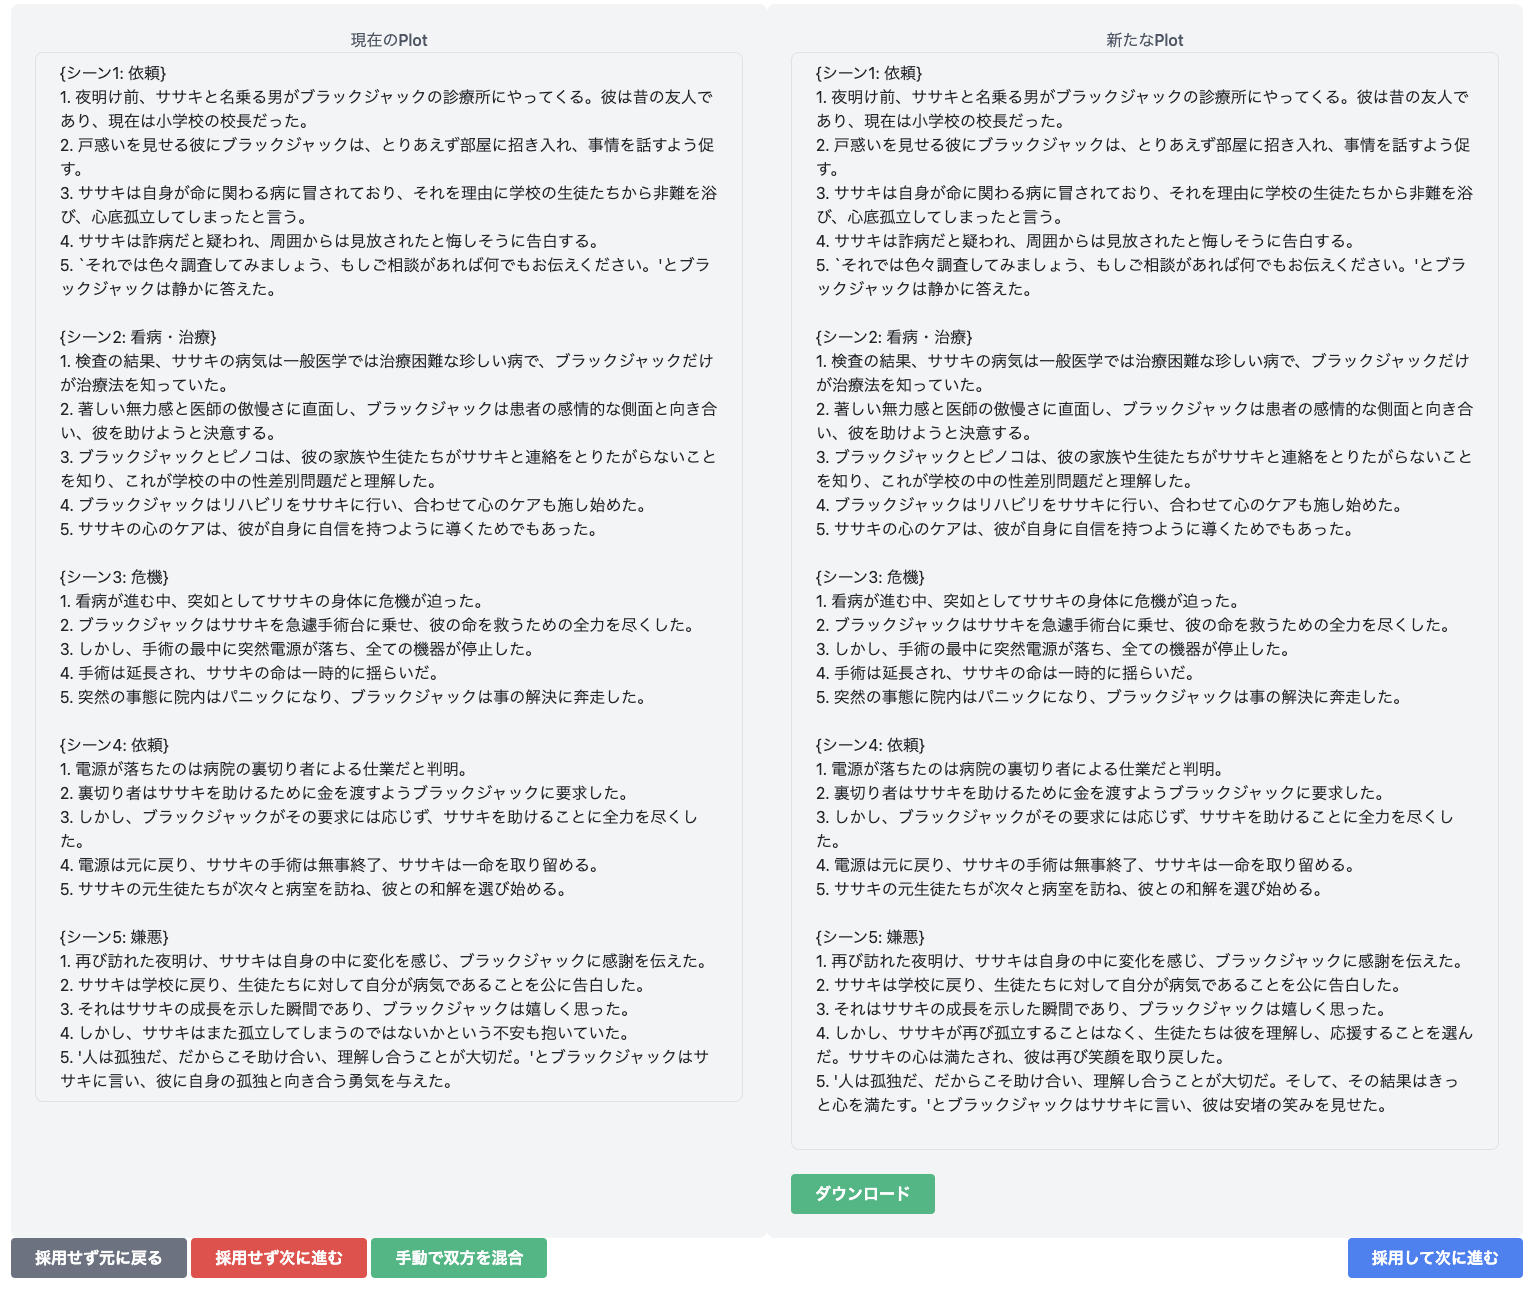
\includegraphics[width=12cm]{pict/04/comparison.png}
   \caption{新旧プロットの比較画面の様子.}
   \label{comparison}
   \end{center}
\end{figure}

\subsection{フリーワードによるやり取り}\label{subsec: freeword}
この機能を用いることでユーザーは, 生成されたプロットについて自由記述により LLM とやり取りを行うことができる. 自身の言葉でプロットに対する質問を投げかけることや, 新たな指示によりプロットを書き換えることができる.

この機能は筆者と他数名により提案されたものである.

図\ref{freeword}に, フリーワードによるやり取りの様子を示す. 図\ref{freeword}で示したように, 既存のプロットを上部に見ながら, その下に配置されているテキストエリアへの入力で, プロットに対する質問, プロットを書き換える指示を行うことができる. 質問は連続して行うことができ, また, 「ダウンロード」ボタンをクリックすることで質問の回答をテキストデータとして保存することもできる. 

質問を投げかけることで得られるLLMからの回答を基に, 新たな指示が想起されることなどが考えられ, この機能はLLMとのインタラクティブ手法として機能する. ストーリークリエーターの自由指示がより効果的に反映されるような工夫が施されており, ストーリークリエーターの創作を支援する.

\begin{figure}[H]
   \begin{center}
   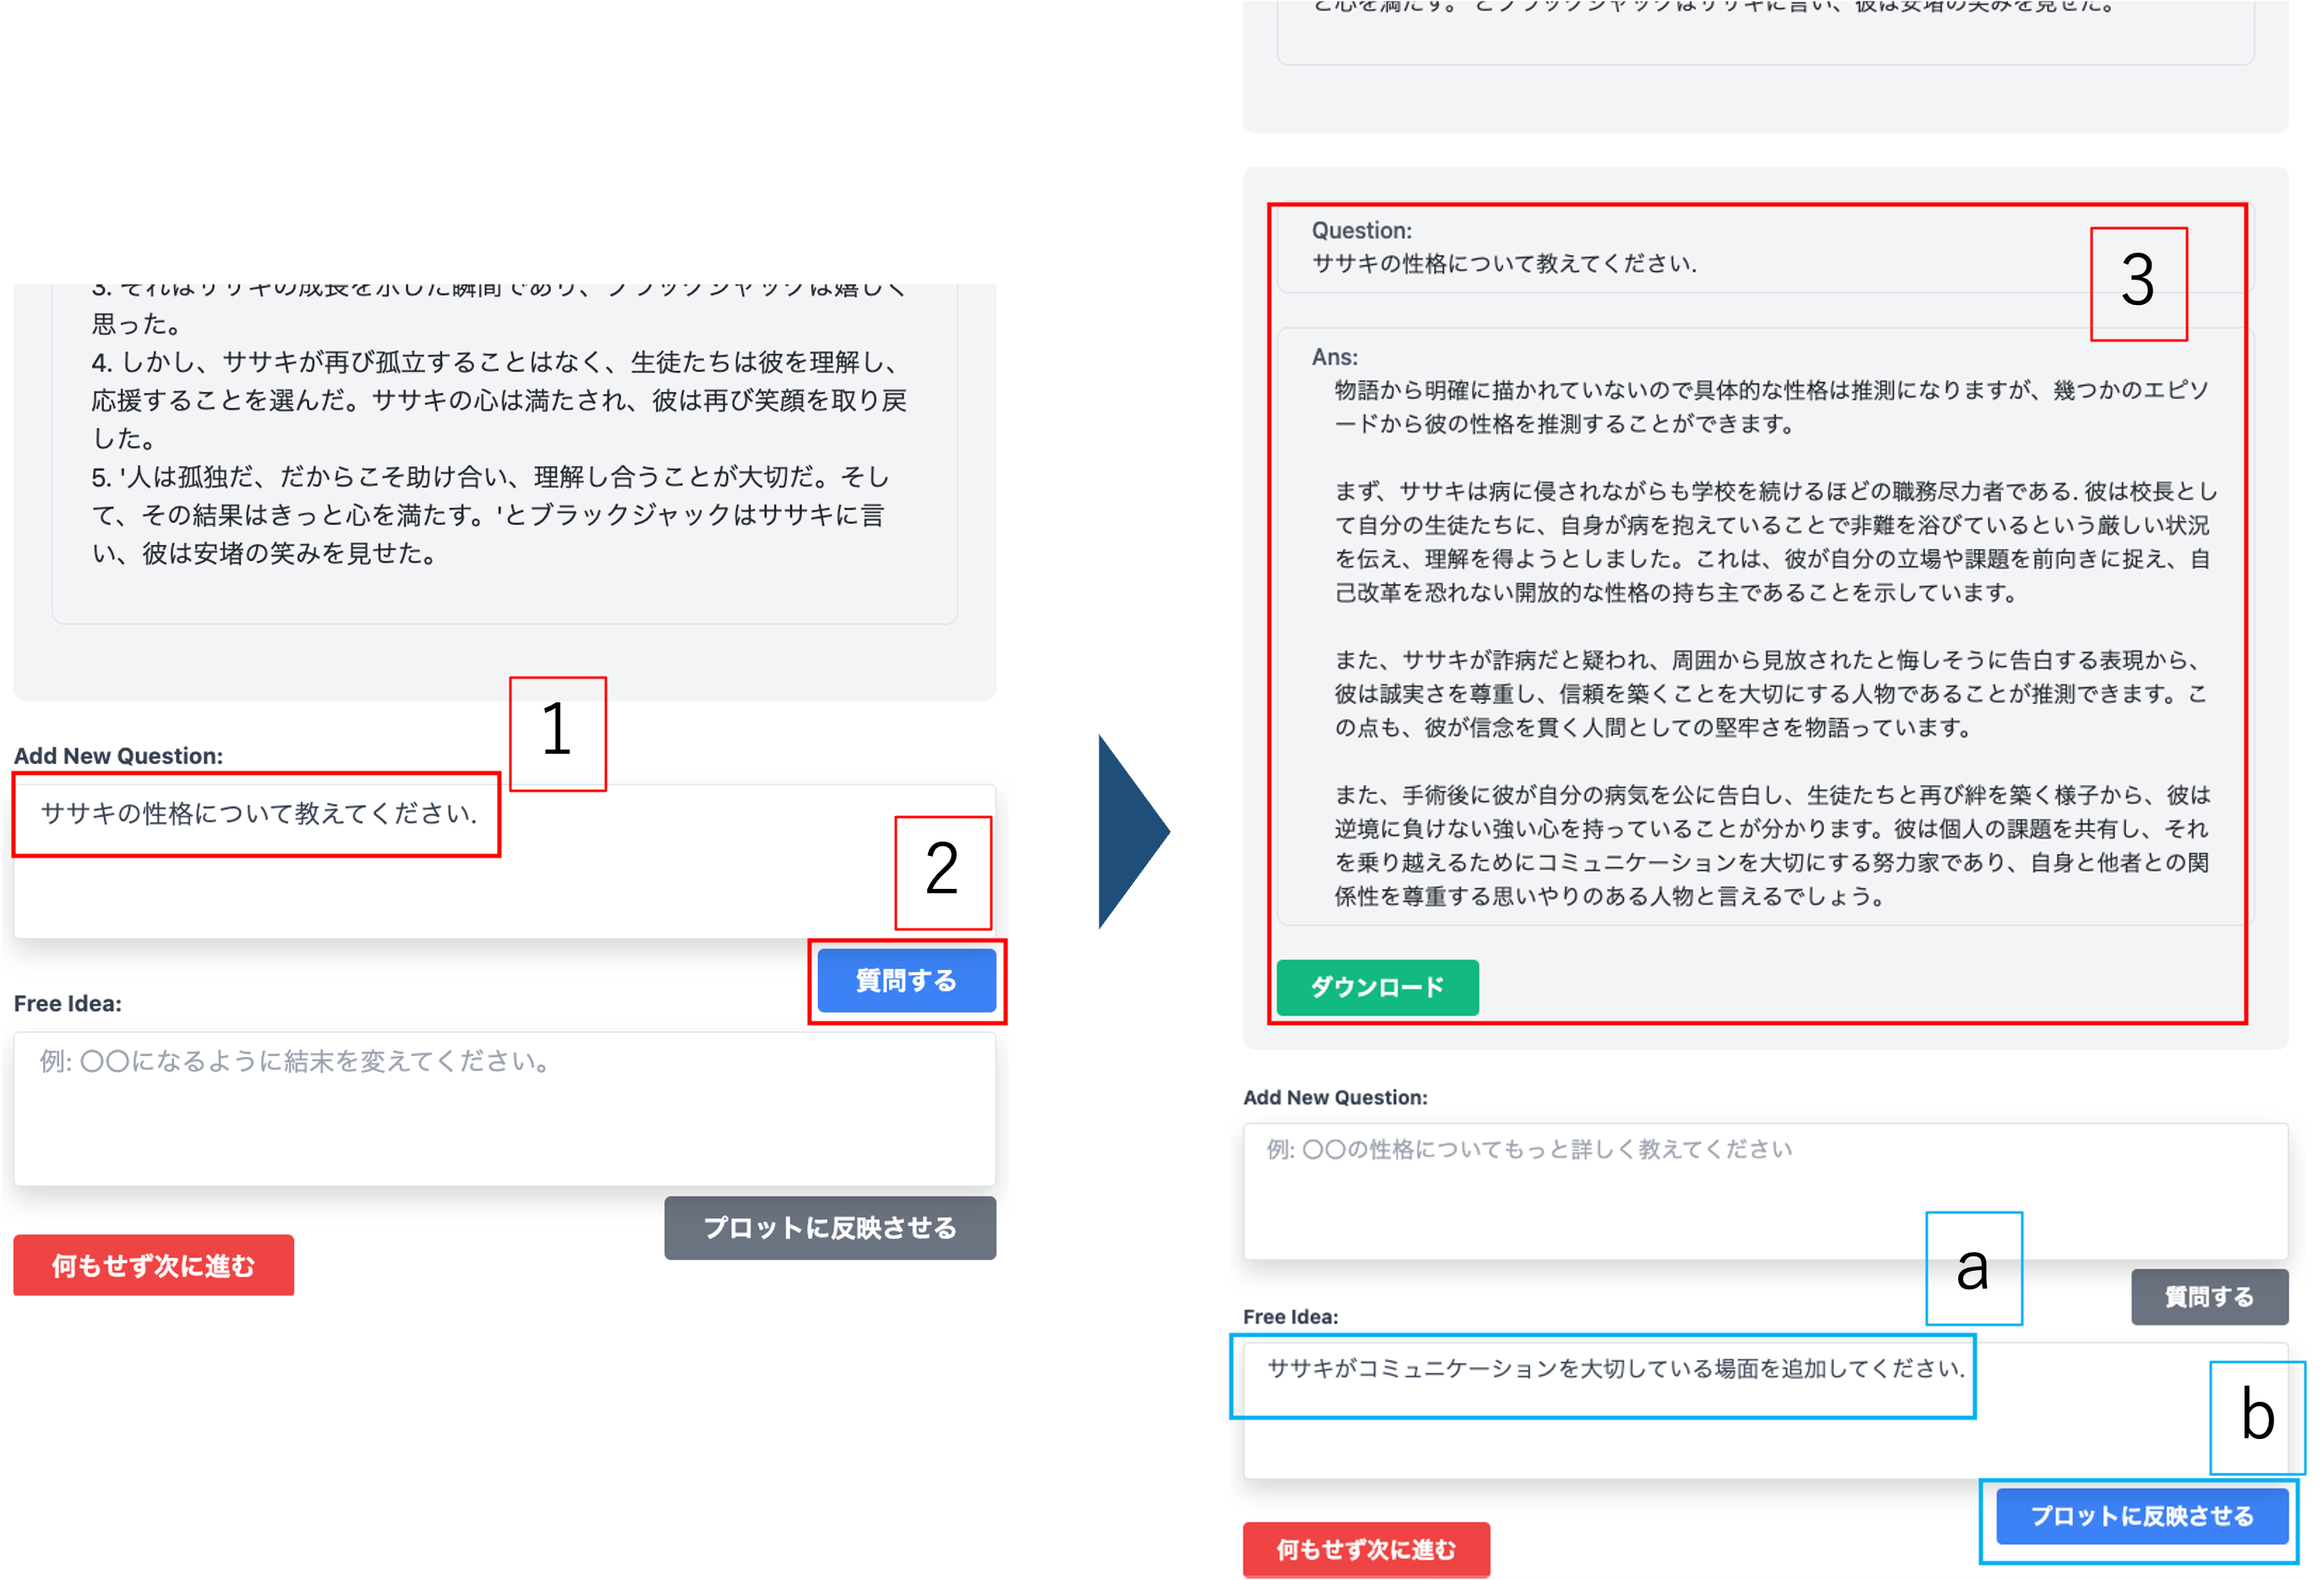
\includegraphics[width=12cm]{pict/04/freequestion.png}
   \caption[フリーワードによるやり取りの様子]{フリーワードによるやり取りの様子. \small (1): プロットに対する質問をテキストエリアに入力. (2):「質問する」ボタンを押すと質問がLLMへ投げかけられる. (3): 回答が出力される. (a): プロットを書き換えるための指示を入力. (b):「プロットに反映させる」ボタンを押すことで指示を反映し書き換えらたプロットが生成され新旧プロットの比較画面へと遷移.}
   \label{freeword}
   \end{center}
\end{figure}

\subsection{プロット中の単語・文章に関する質問}
\label{subsec: question}
この機能は, プロットの中に書かれた, 説明が不十分であると思われる単語や, 内容をより深掘りしたいと思う文章について, LLMを介しその詳細な説明と解釈の例を回答として得ることができる機能である.

図\ref{question}にこの機能の操作画面の様子を示す. この機能は図\ref{question}に示したように, コピーアンドペーストとクリック操作のみで利用でき, クリエーターの負担を軽減する. 単に質問を投げかけるだけでは, プロットに書かれていること以上の内容が回答に含まれないため, プロットに書かれいている範囲の外のことも含め回答がなされるよう工夫も施している.

この機能では, 得られた回答を用い新たなプロットを生成させることもでき, インタラクティブなプロット創作を実現する.

\begin{figure}[H]
   \begin{center}
   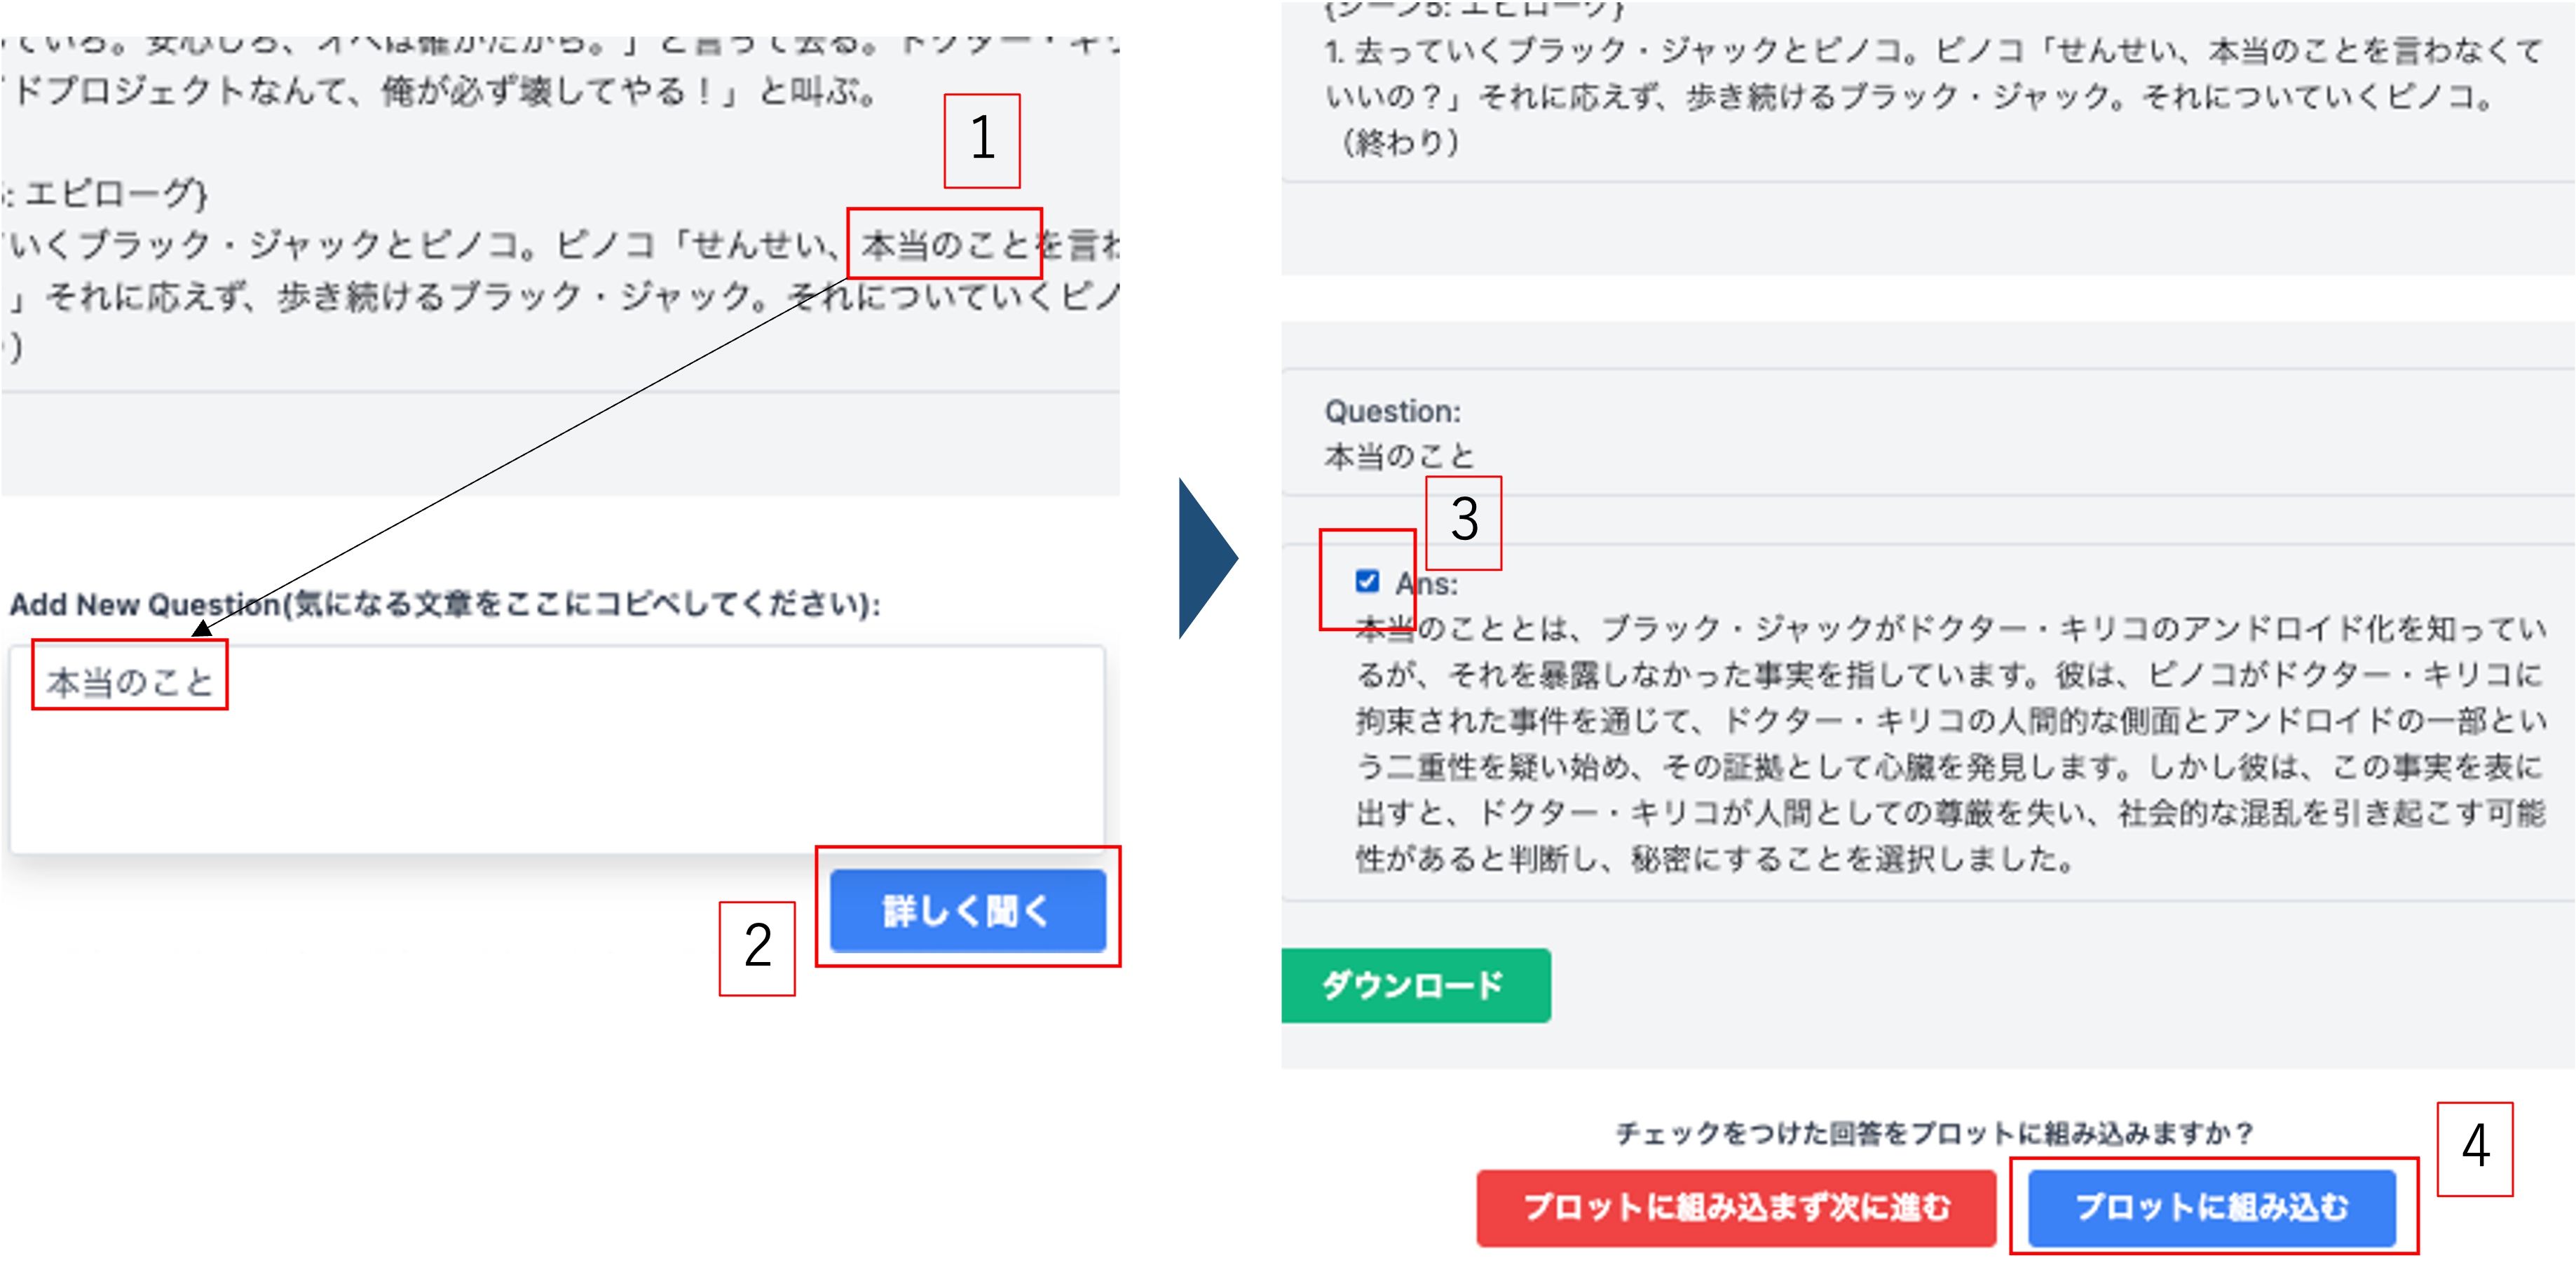
\includegraphics[width=12cm]{pict/04/question00.png}
   \caption[プロット中の単語・文章に関する質問機能実行の様子]{プロット中の単語・文章に関する質問機能実行の様子.\small (1): 内容をより詳しく知りたいプロット上の単語や文章をテキストホルダーに入力する. (2): 詳しく聞くをクリックすると(1)で入力したものを深掘りした文章が生成される. (3): 回答にチェックをつける. (4): プロットに組み込むを押すと(3)でチェックをつけた回答が反映したプロットに書き換えられプロットの比較画面へと遷移する.}
   \label{question}
   \end{center}
   \end{figure} 


\subsection{アイデア生成}
\label{subsec: idea}
この機能は, 既存のプロットを読み込んだLLMに, そのプロットで用いることができそうなアイデアを生成させることができる機能である. 

図\ref{ideas_e}に, アイデア生成機能実行の様子を示す. 図\ref{ideas_e}に示したような操作により, 既存のプロットに用いられることが想定されたアイデアを生成させることができ, そのアイデアを用いてプロットを書き換えることができる. アイデアは, 10個ずつ連続して生成させることも可能で, 「ダウンロード」ボタンをクリックすることによりテキストデータとして保存することもできる. 反映させるアイデアはユーザー自身の言葉で入力することも可能であり, LLMが出力したアイデアから想起されたクリエーター自身のアイデアをアウトプットする機会となる. この機能によりストーリークリエーターとLLMとの共創を実現する.

\begin{figure}[H]
   \begin{center}
   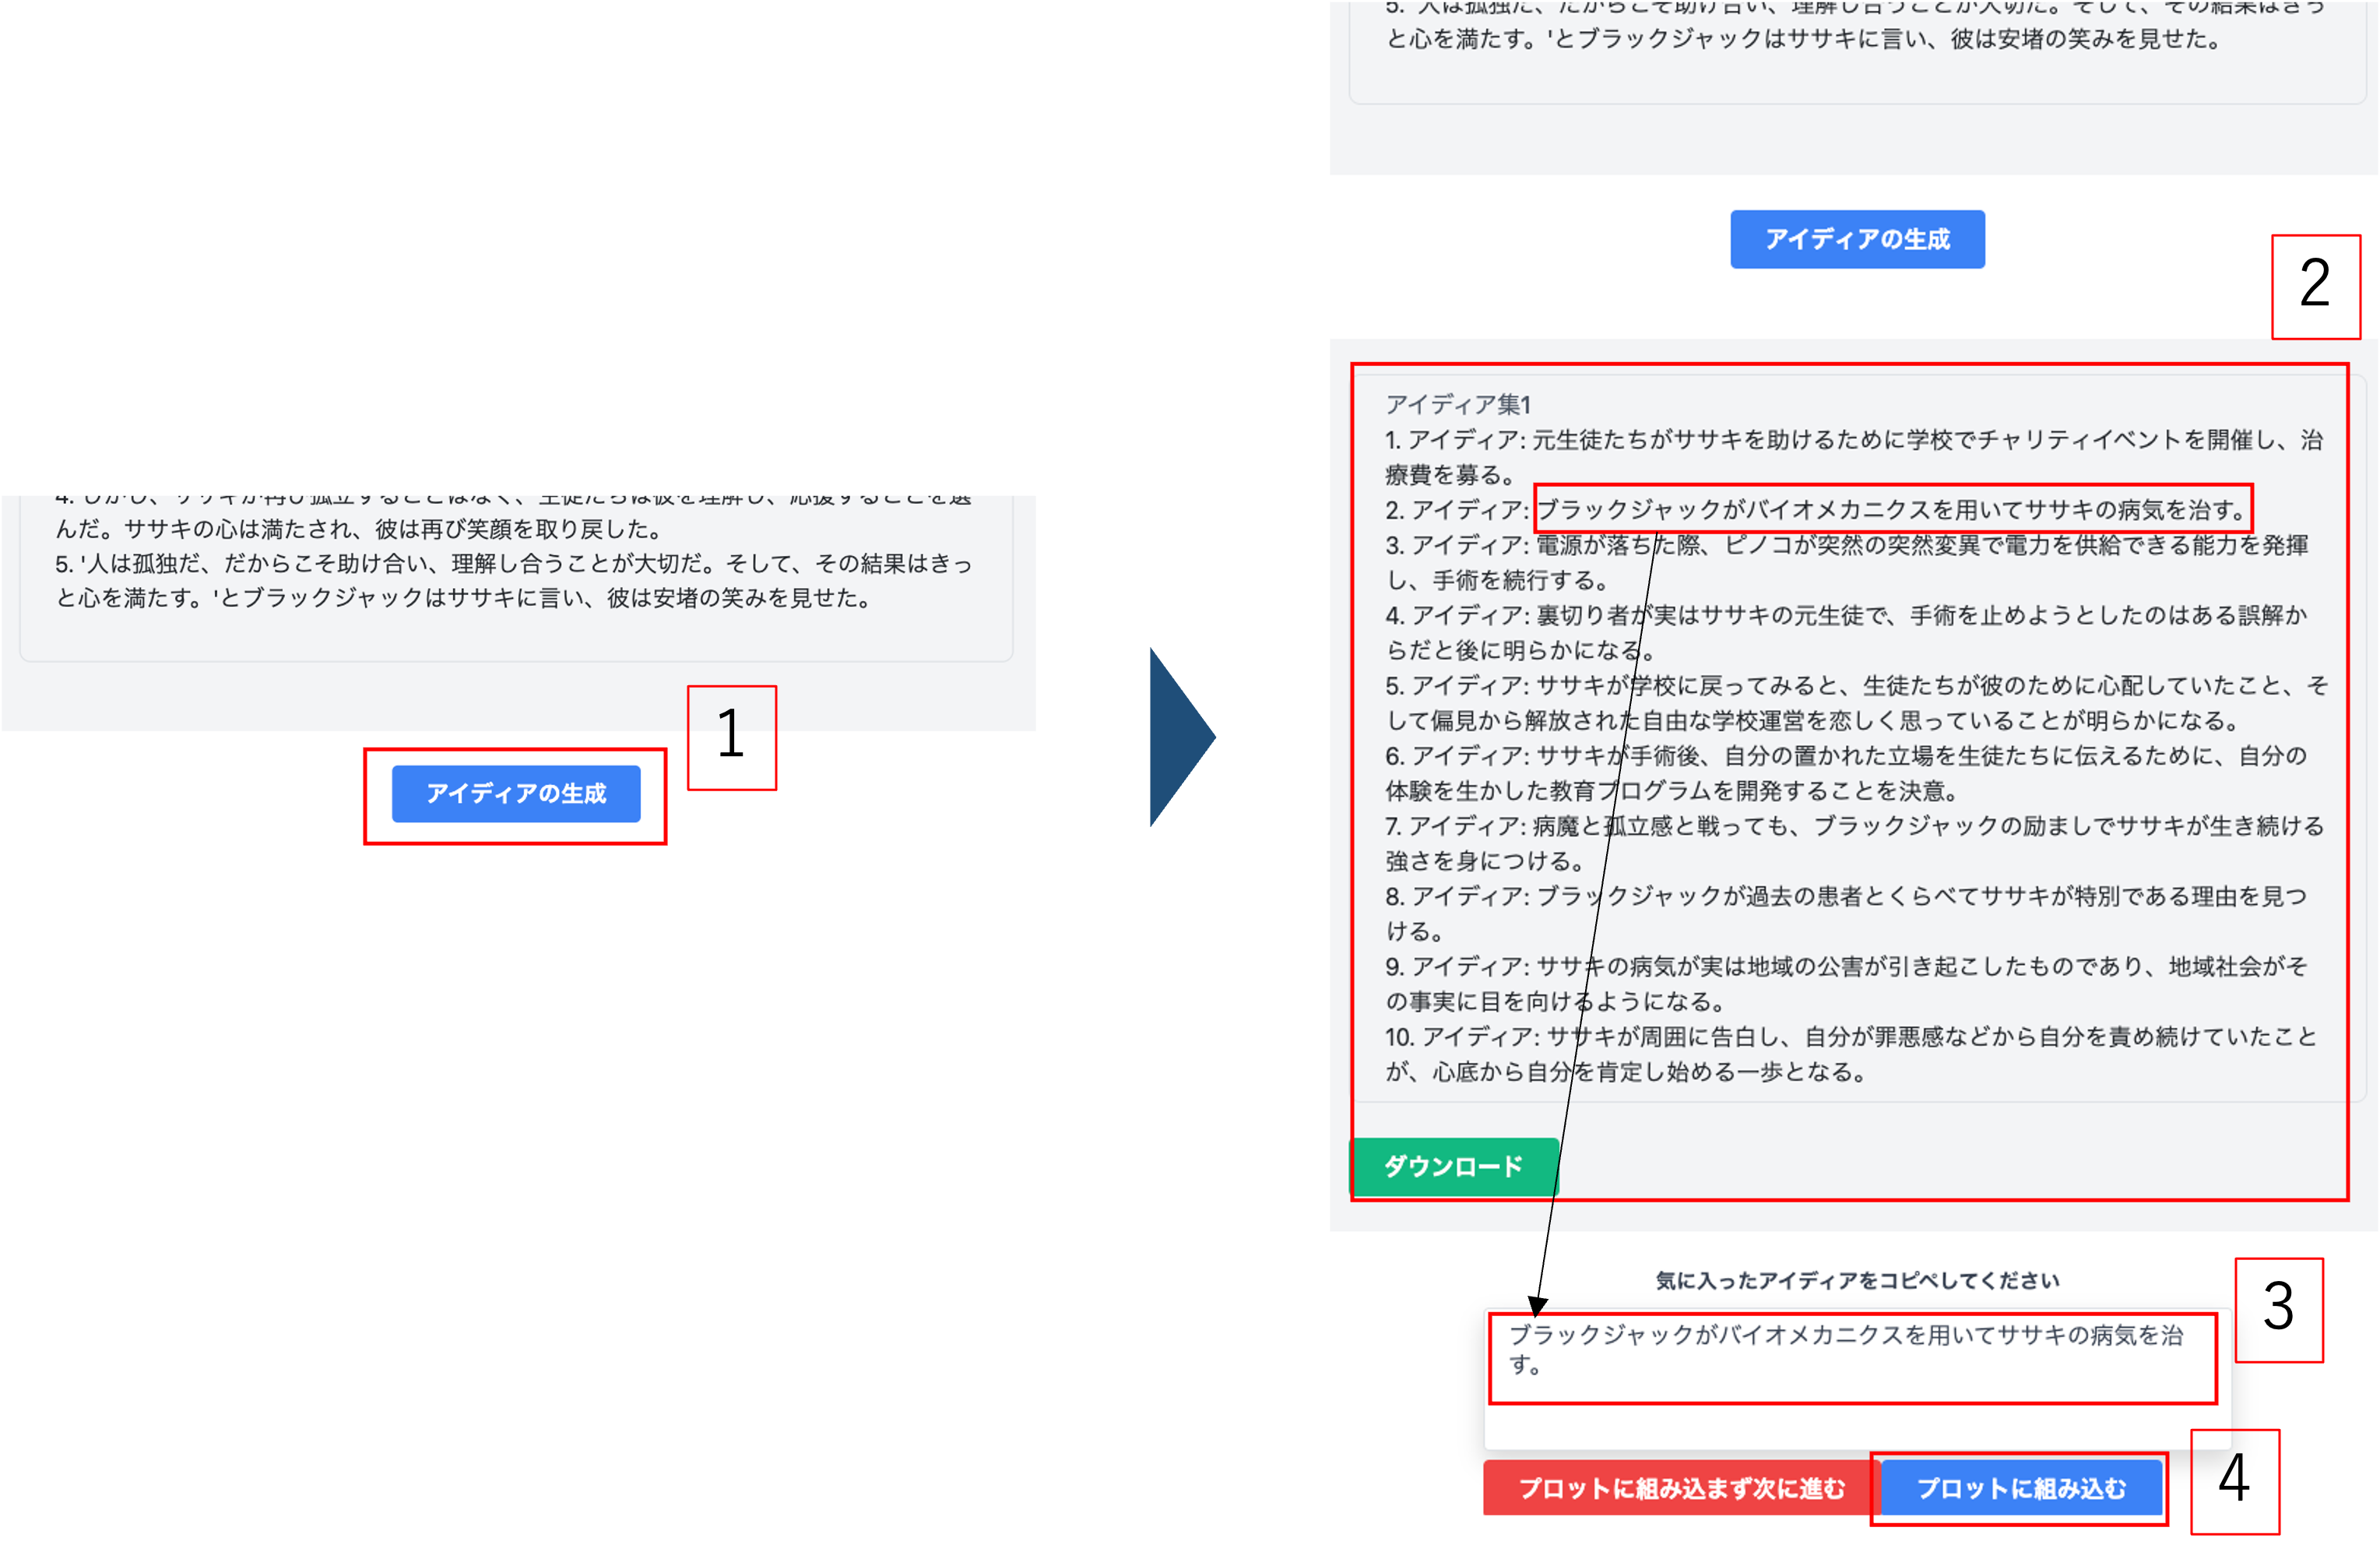
\includegraphics[width=12cm]{pict/04/ideas_e.png}
   \caption[アイデア生成機能実行の様子]{アイデア生成機能実行の様子. \small (1): 「アイデアの生成」ボタンをクリックする (2): アイデアが10個生成される. (3): 生成されたアイデアの中で気に入るアイデアがあればそれを画面下部のテキストエリアへとコピペする. (4): プロットに組み込むを押すと, (3)でコピペしたアイデアがプロットに反映される.}
   \label{ideas_e}
   \end{center}
\end{figure}

\subsection{伏線の処理}
\label{subsec: foreshadowing}
この機能を用いることにより, ユーザーは既存のプロットの中で起こる出来事について, その伏線をその出来事が起こる前のシーンに張ることができる. これにより, 物語の一貫性を保ちつつ, 物語に複雑性を持たせることができる. また, 生成されるプロットを一つの例として, ストーリー創作における伏線についてのアイデアを獲得することができる.

 図\ref{foreshadowing}に, 伏線処理機能を実行している様子を示す. 図\ref{foreshadowing}に示したように簡便な操作を実行することで, 伏線が張られたプロットをLLMを介し生成させることができる. 

 伏線は, 物語に説得力や複雑性, エンタテイメント性を与えると考えられるが, 物語の整合性を保ち伏線を処理することは難しい. 上記のような簡便な操作でその一例を直ちに取得できるこの機能は, ストーリークリエーターの創作を支援すると考えられる.

\begin{figure}[H]
   \begin{center}
   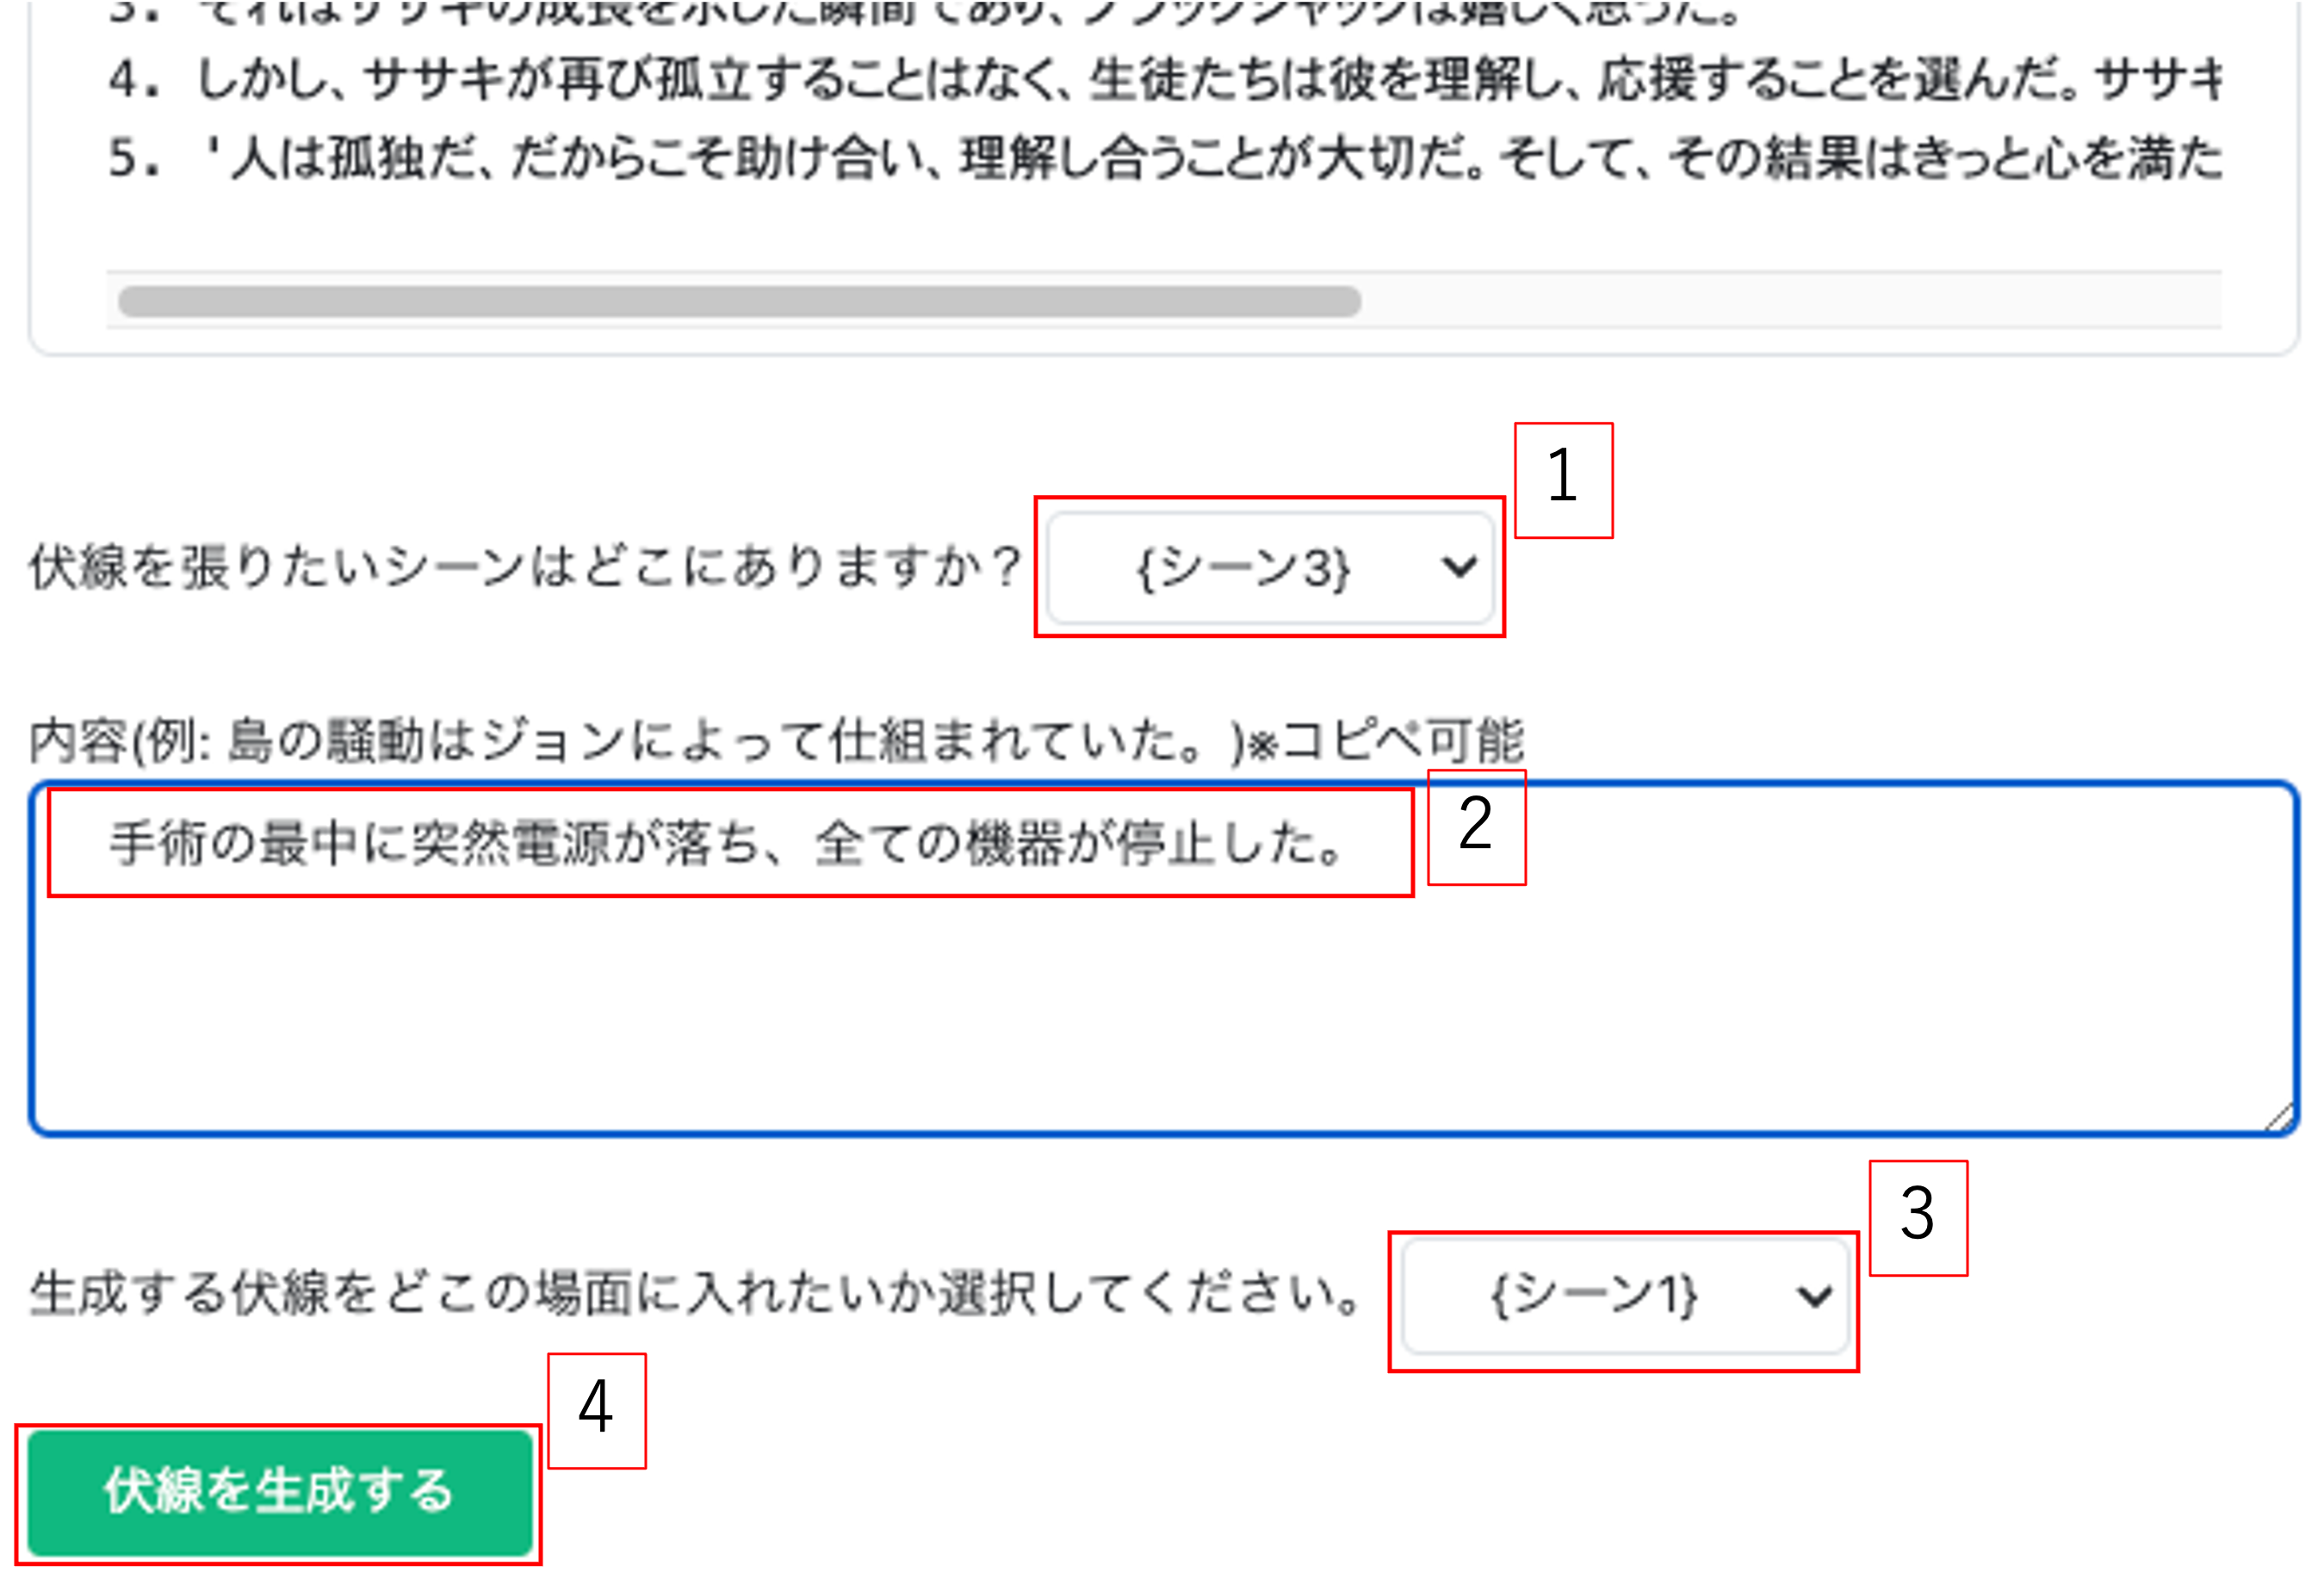
\includegraphics[width=9cm]{pict/04/foreshadowing.png}
   \caption[伏線の処理機能を実行する様子]{伏線の処理機能を実行する様子. \small (1): 伏線を張りたいシーンがどのシーンにあるかシーン番号で選択. (2): 伏線を張りりたいと思う内容をプロットからコピペするなどしてテキストエリアに記述. (3): 伏線を張るシーン番号を選択. (4): 「伏線を生成する」ボタンをクリックすると, 伏線が張られたプロットが生成され, 新旧プロットの比較画面へと遷移.}
   \label{foreshadowing}
   \end{center}
\end{figure}

\subsection{一部シーン変更}
\label{subsec: change}
この機能は, 選んだシーンの内容を変更することができる機能である. 他のシーンを変えることなく選択したシーンの内容のみを変更することができ, 変更されたシーンが, 矛盾なく前後のシーンと繋がり, プロットとしての一貫性が保たれるよう工夫を施した. 操作は単純で, 変更したいシーンの横にあるチェックボックスにチェックを入れるだけで良い. 操作の簡便性によりクリエーターの負担を軽減する. 図\ref{change}に, 一部シーン変更機能を実行している様子を示す.

\begin{figure}[H]
   \begin{center}
   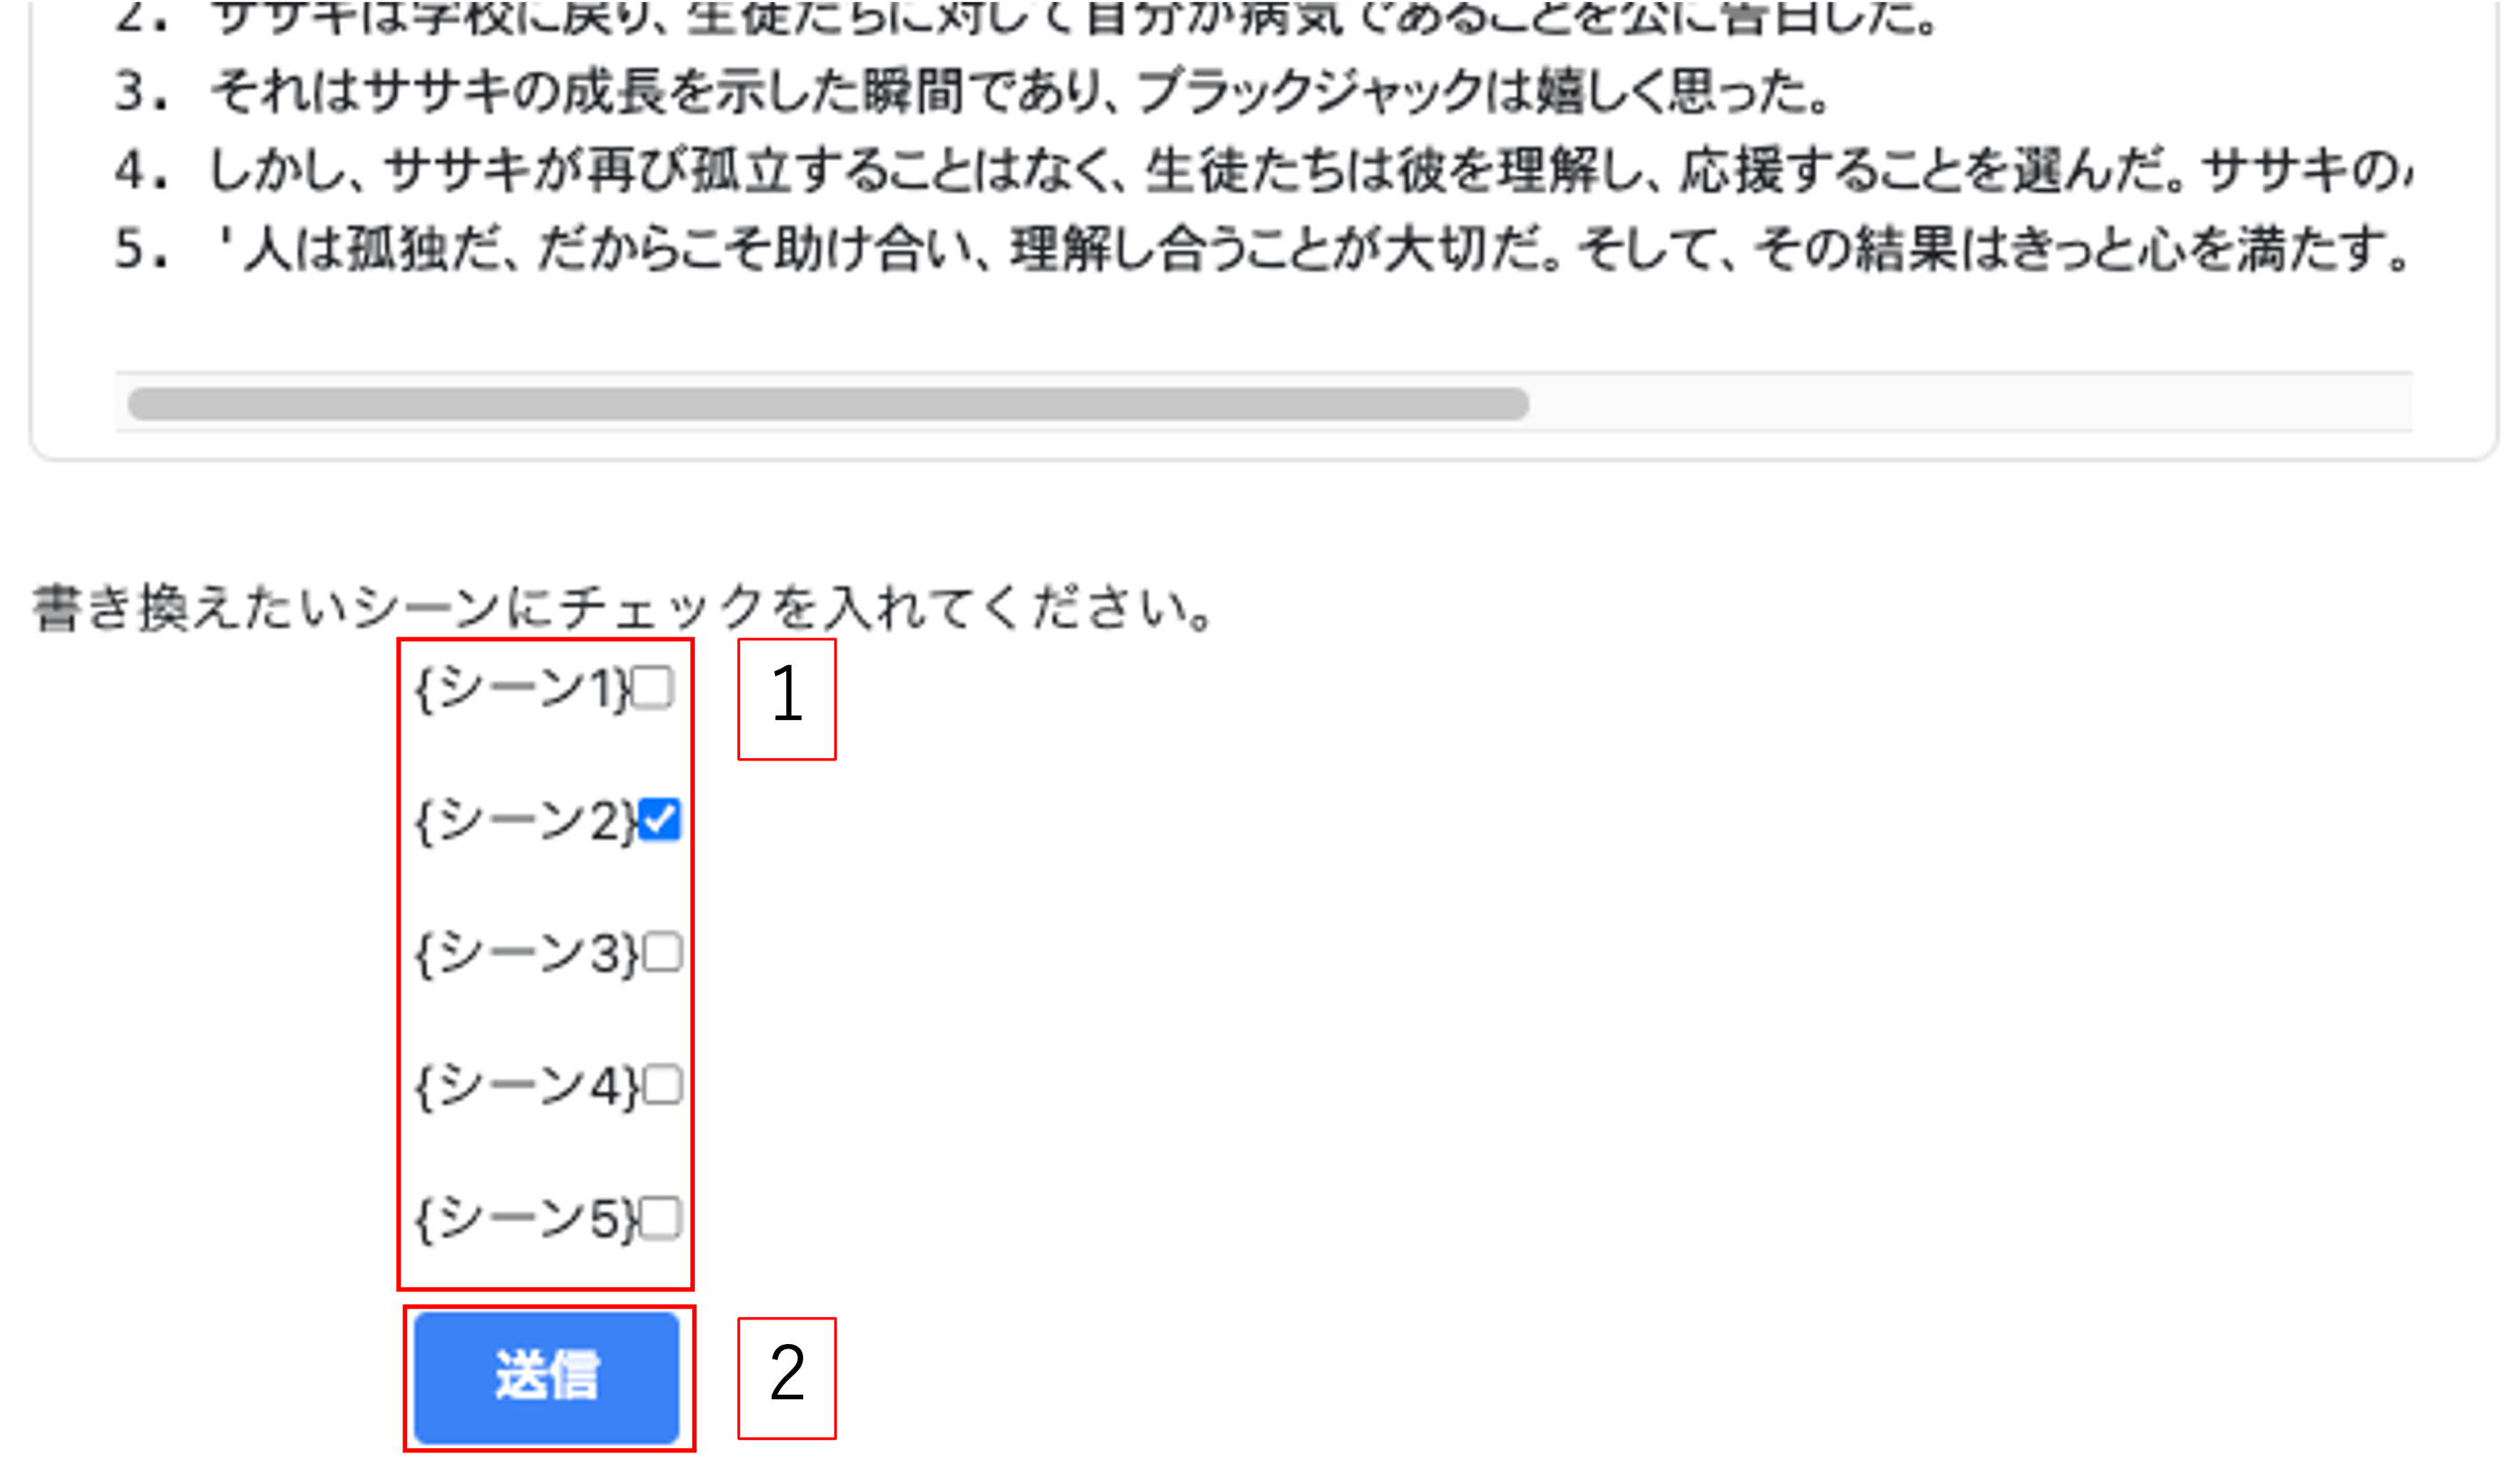
\includegraphics[width=10cm]{pict/04/change.png}
   \caption[一部シーン変更機能を実行する様子]{一部シーン変更機能を実行する様子. \small (1): 変更したいシーンのチェックボックスにチェックを入れる. (2): 「決定」ボタンを押すと, 選択したシーンのみが変更されたプロットが生成され, 新旧プロットの比較画面へと遷移する.}
   \label{change}
   \end{center}
\end{figure}

\subsection{全体的な雰囲気の変更}
\label{subsec: atmosphere}

この機能は, 指定した雰囲気になるようプロットを書き換えることができる機能である. ユーザー自身がプロットに対する具体的なアイデアを持っていないが, 生成したいと考えるプロットの雰囲気やイメージは持っているという場合に利用されることを想定している. この機能を利用することで, そうしたイメージを具体化する一つの例を獲得することができる. これはストーリークリエーターの創造性の拡張に繋がり, 創作支援に役立つものと考えられる. 図\ref{atmosphere}にこの機能の操作画面の様子を示す. 図\ref{atmosphere}に示した通り, 直感的な操作によりこの機能を実行することができ, クリエーターの負担を軽減する.

\begin{figure}[H]
   \begin{center}
   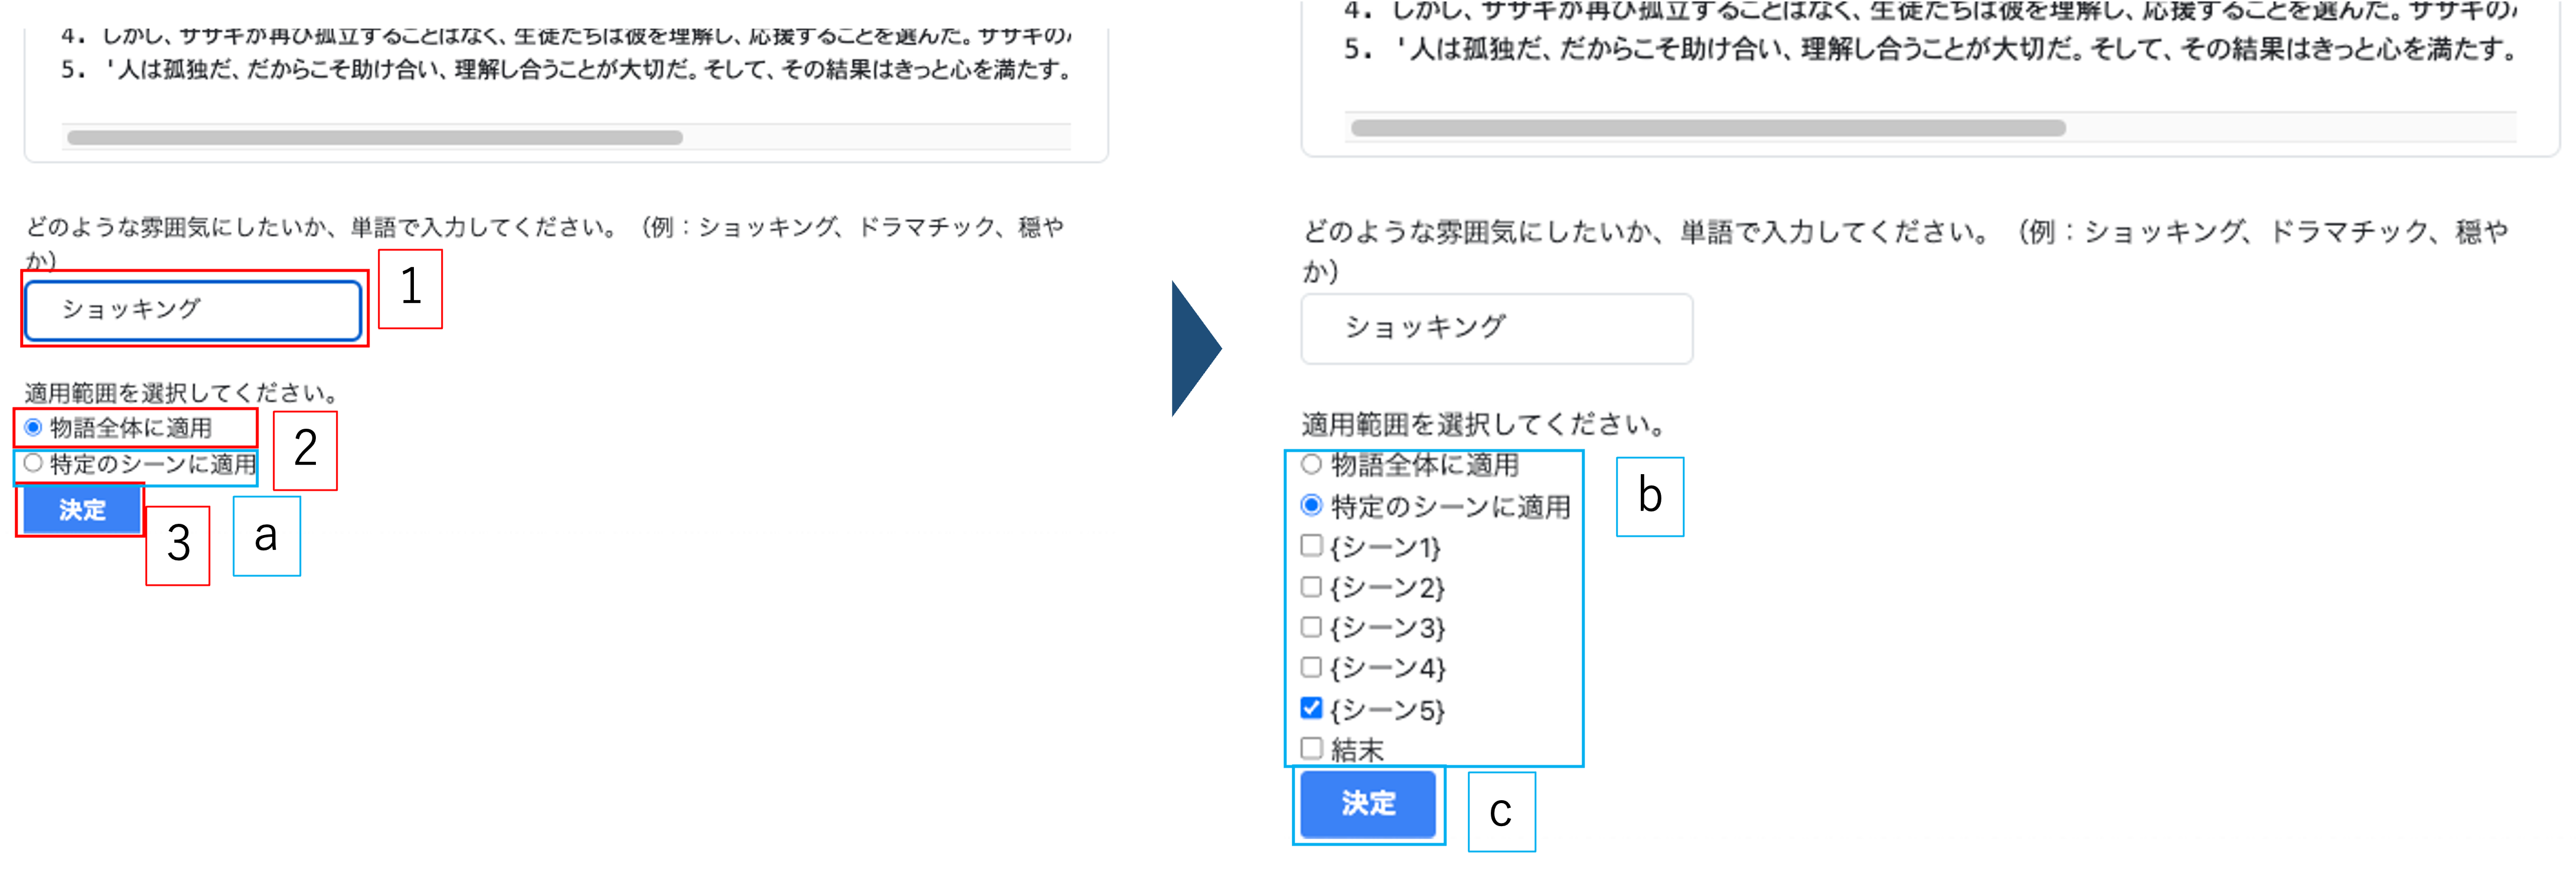
\includegraphics[width=12cm]{pict/04/atmosphere.png}
   \caption[全体的な雰囲気の変更機能を実行する様子]{全体的な雰囲気の変更機能を実行する様子. \small (1): テキストエリアにどのように雰囲気を変更したいかを入力する. (2): 雰囲気の変更を「物語全体に適用」するか「特定のシーンに適用」するかを選択する. (3): 「決定」ボタンを押すと, 入力した雰囲気になるよう書き換えられたプロットが生成され, 新旧プロットの比較画面へと遷移する. (a): 「特定のシーンに適用」するとどのシーンに適用するかを選択するためのチェックボックスが展開される. (b):  雰囲気を変更したいシーンにチェックをいれる. (c): 「決定」ボタンを押すと, 選択したシーンの雰囲気のみが, 入力した雰囲気になるようプロットが書き換えられ, 新旧プロットの比較画面へと遷移する.}
   \label{atmosphere}
   \end{center}
\end{figure}

\subsection{シーンの入れ替え}
\label{subsec: swap}
この機能は, 物語の流れを変えずに, 物語の中の出来事の順番を入れ替えることができる機能である.

LLMが生成する物語は時系列の順に描かれる傾向にある. しかしながら, 物語は必ずしも時系列の順に書かれる必要はなく, むしろ出来事を描く順番を入れ替えることで, 物語の面白さを高めることができる場合もある. この機能は, 物語の面白さを高めるため, 出来事が描かれる順番を入れ替えた一例を獲得することができる機能であり, 創作支援として役立つものと考えられる.

この機能を操作している様子を図\ref{swap}に示す. 図\ref{swap}に示した通り, テキストエリアへの入力も, 画面上部に表示される既存のプロットからコピーアンドペーストし入力するだけで済むため, ストーリークリエーターの負担を軽減し, 創作支援になると考えられる.

\begin{figure}[H]
   \begin{center}
   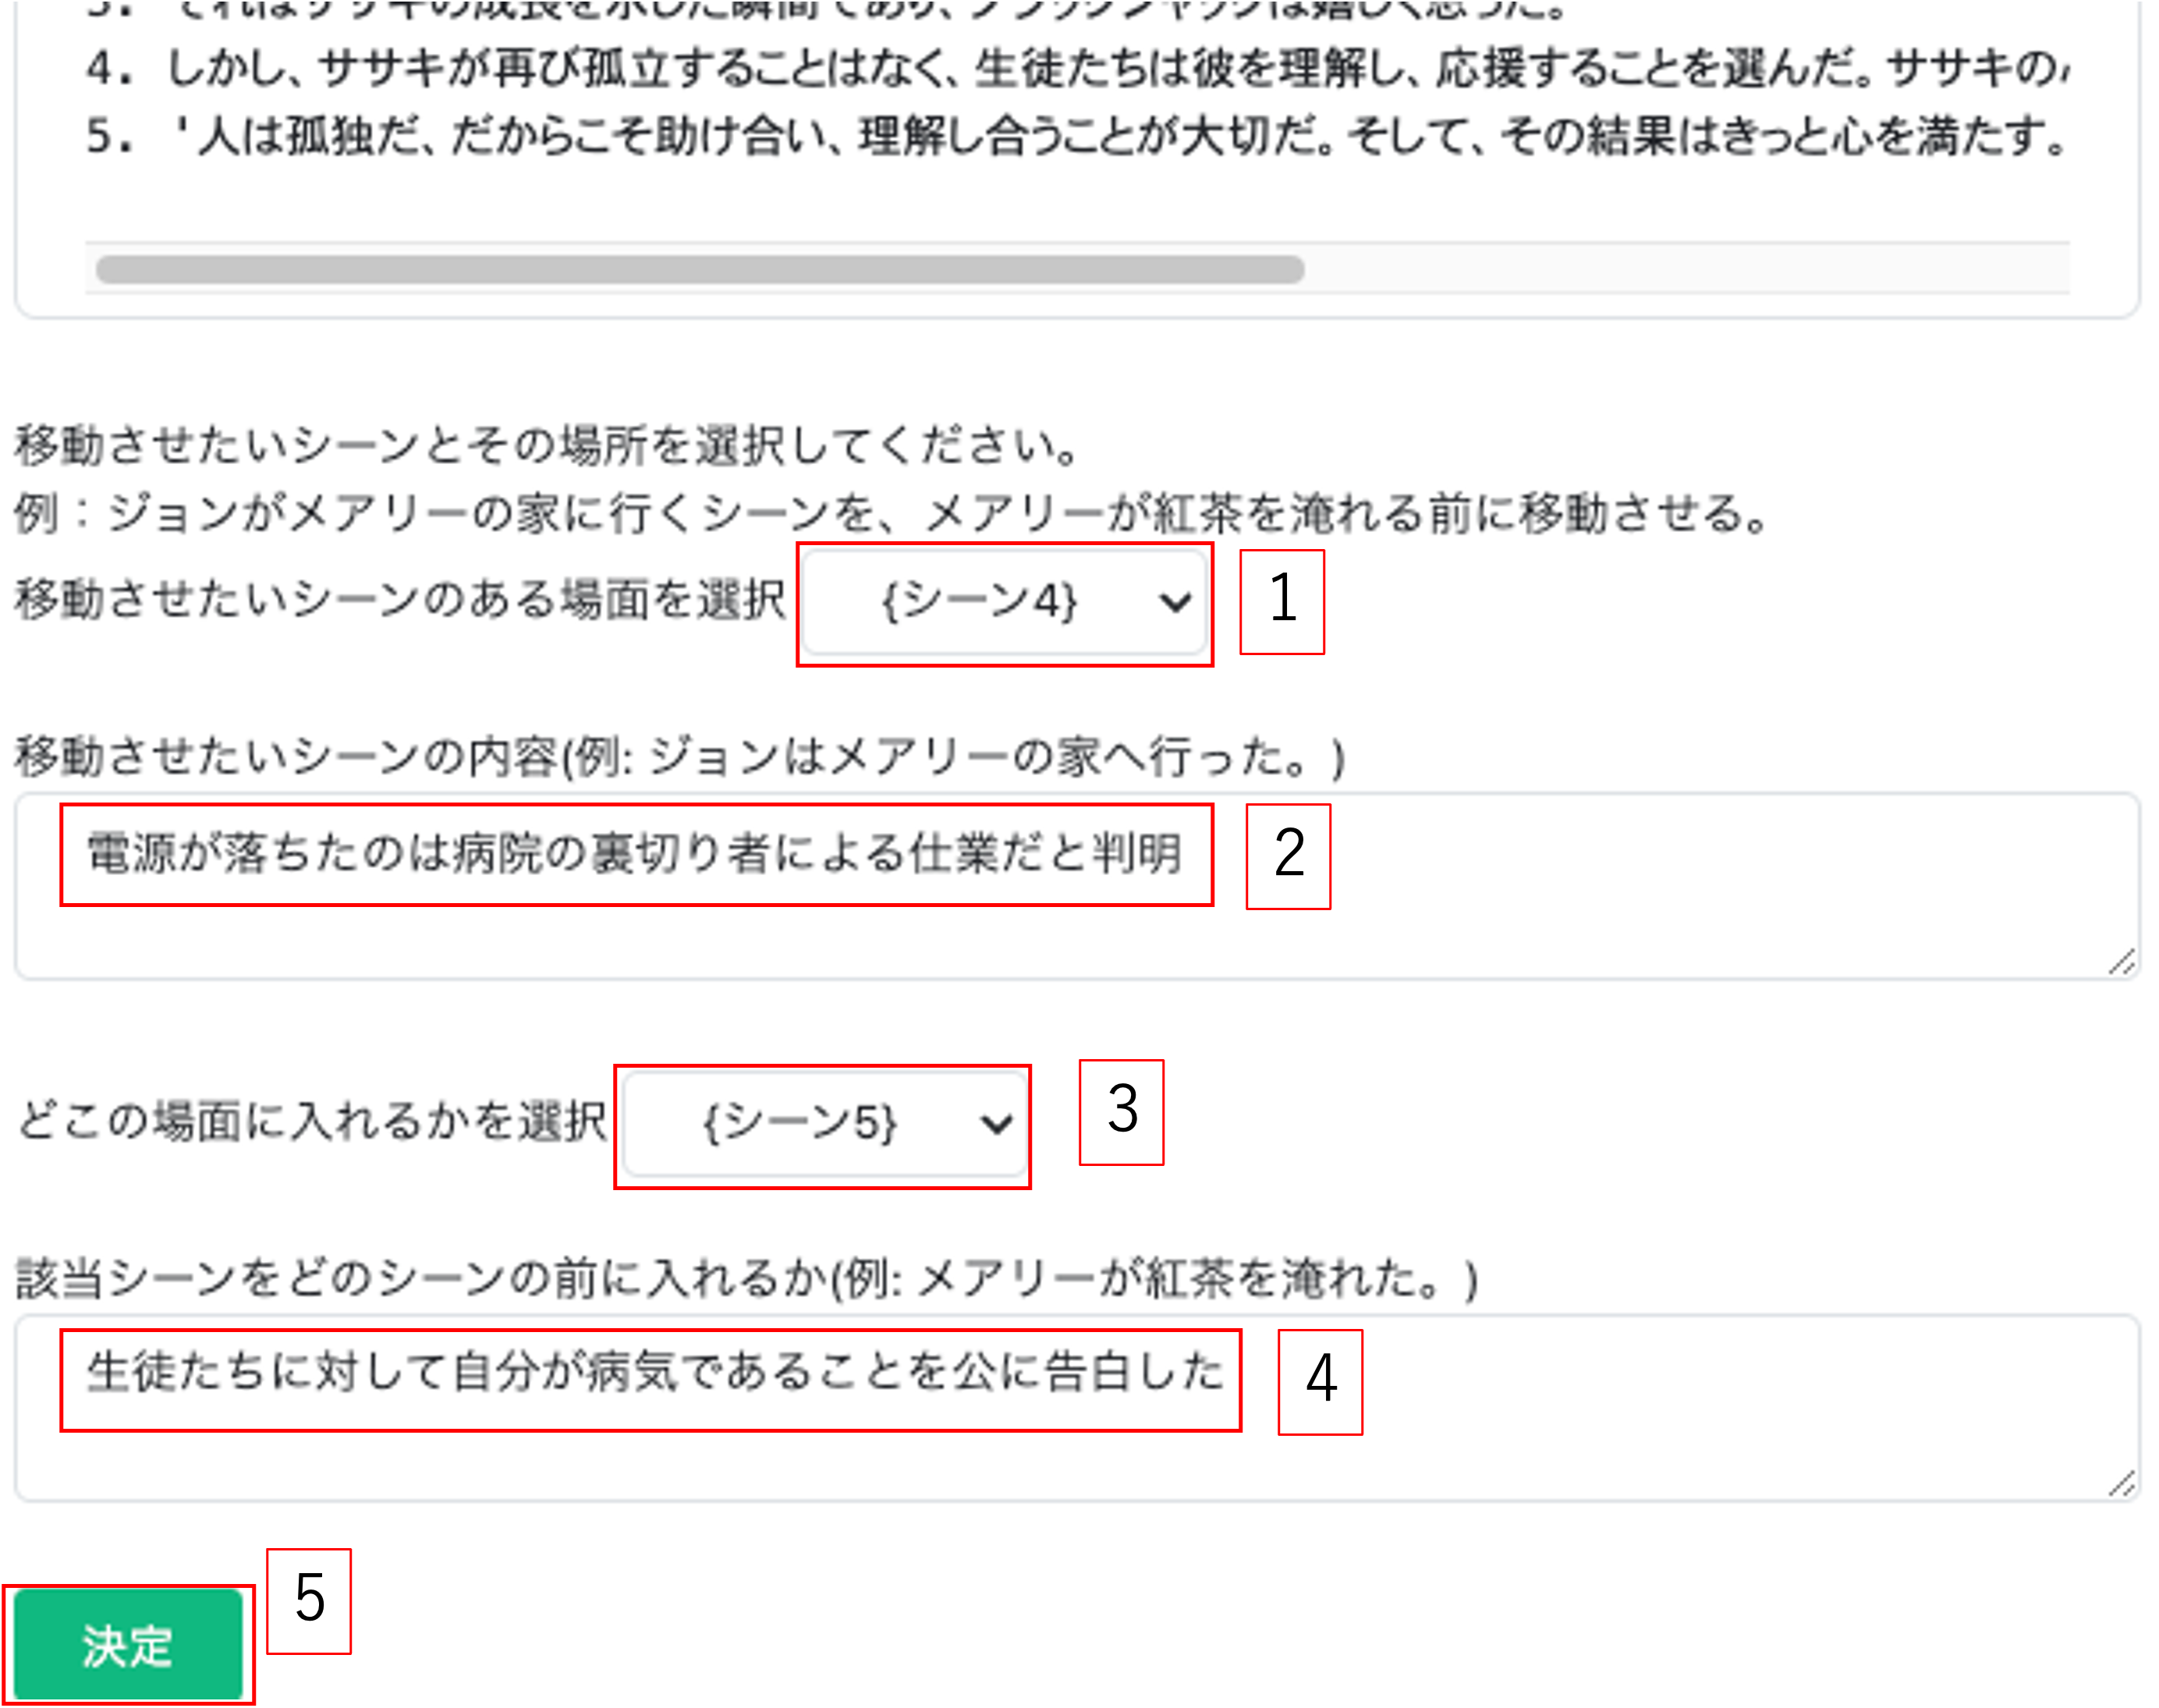
\includegraphics[width=9cm]{pict/04/swap.png}
   \caption[シーンの入れ替え機能を実行する様子]{シーンの入れ替え機能を実行する様子. \small (1): 移動させたい出来事がどのシーンに含まれるかを選択する. (2): その出来事の内容をコピーアンドペーストなどを用いてテキストエリアに入力する. (3): その出来事をどのシーンに移動させて以下を選択する. (4): そのシーンの中のどの出来事の前に移動させたいかをテキストエリアにコピーアンドペーストなどを用いて入力する. (5): 「決定」ボタンを押すことにより, その出来事が移動したプロットが生成され, 新旧プロットの比較画面へと遷移する.}
   \label{swap}
   \end{center}
\end{figure}

\subsection{シーンごとの視点の変更}
\label{subsec: perspective}

この機能は, プロット生成セクションにおける主観視点の設定と同様で, 各シーンを指定した登場人物の視点から描くようプロットを書き換えることができる機能である.

各シーンにおける主観視点の設定は, ストーリークリエーターの方から頂いた意見のもと実装した機能であり, それぞれの立場から物語を描くことには, 物語に深みと複雑性を持たせる狙いがある. この機能を用い物語の目線を変えることで, 既存のプロットに対し新たな気づきを得られることが期待され, これは創作支援に役立つものと考えられる.

この機能を操作している様子を図\ref{perspective_e}に示す. 図\ref{perspective_e}に示した通り, 操作はテキストエリアへの名前の入力とボタンを押すことだけでよく, 視点を変えたプロットの生成を, このような容易な操作により実現することでストーリークリエーターの創作を支援する.

\begin{figure}[H]
   \begin{center}
   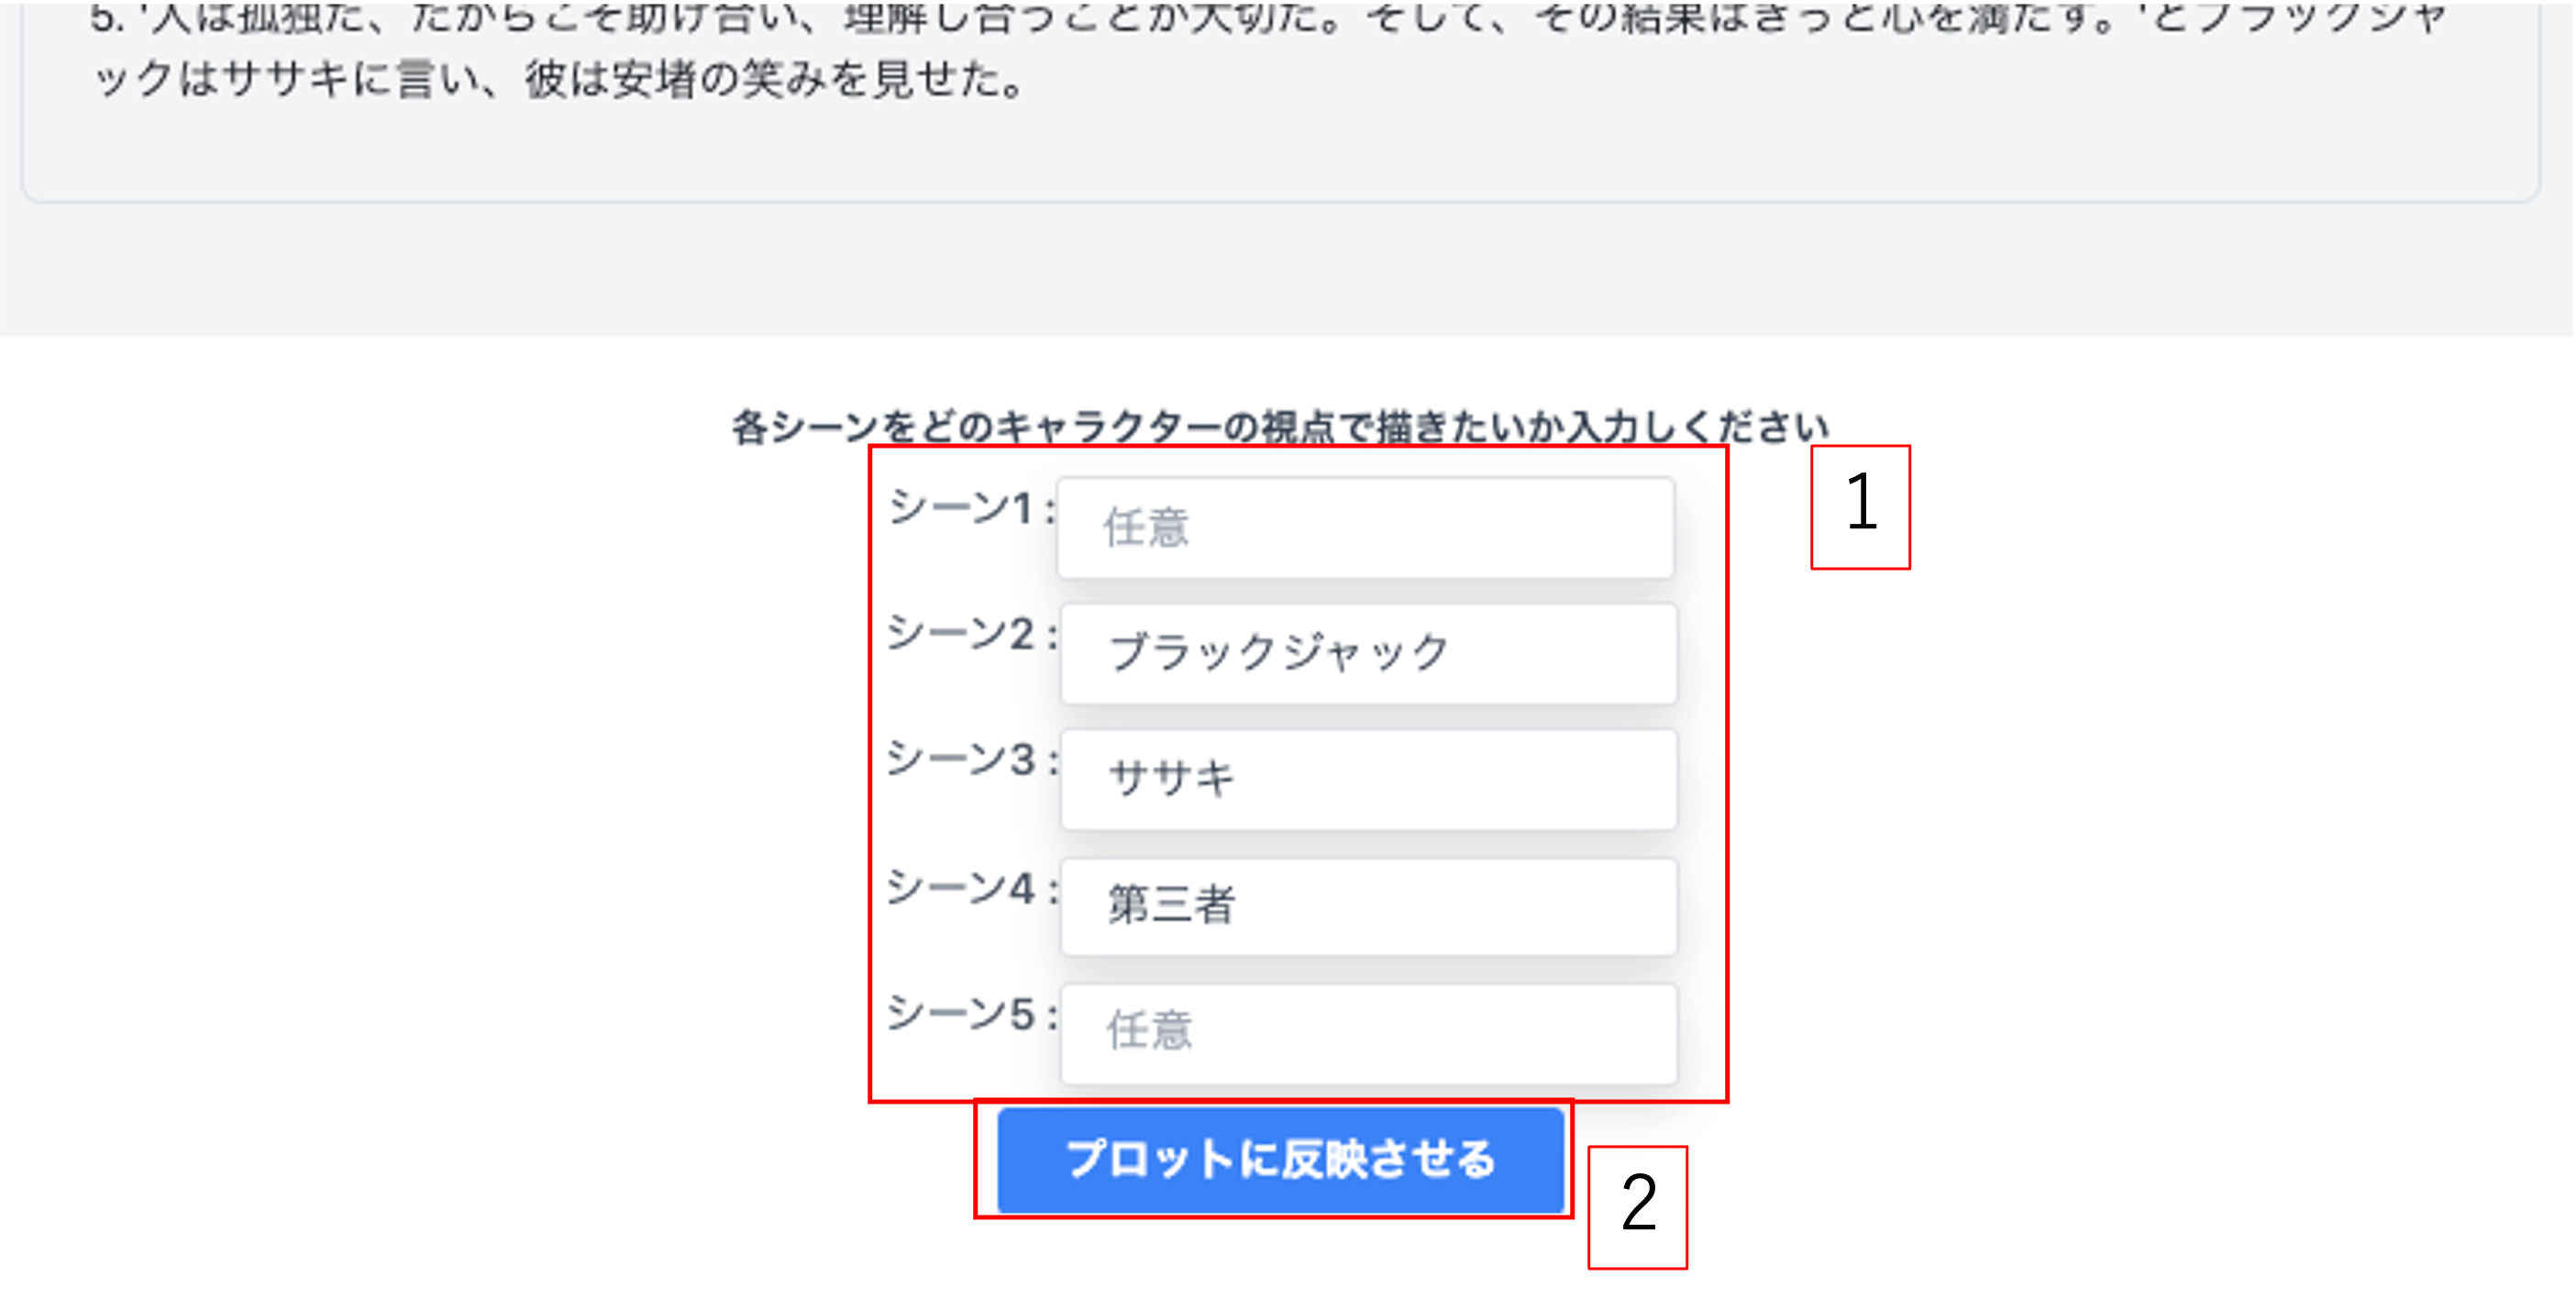
\includegraphics[width=12cm]{pict/04/perspective_e.png}
   \caption[シーンごとの視点の変更機能を実行する様子]{シーンごとの視点の変更機能を実行する様子. \small (1): 視点を変更するシーンのテキストエリアに登場人物の名前を入力する. (2): 「プロットに反映させる」ボタンを押すことで, 指定した視点でシーンが書き換えられたプロットが生成され, 新旧プロットの比較画面へと遷移する.}
   \label{perspective_e}
   \end{center}
\end{figure}


\subsection{登場人物の追加}
\label{subsec: add}
この機能は既存のプロットに新たな登場人物を追加するための機能である. この機能を用いることで, 新たな登場人物を加えた場合, プロットがどのように書き換えられることになるか, その一例を容易に獲得することができ, これは創作支援に役立つものと考えられる.

この機能を操作している様子を図\ref{add}に示す. 図\ref{add}に示した通り, 操作はプロット生成セクションにおける新規キャラクターの追加とほとんど同じように行うことができ, 『ブラック・ジャック』の物語構造分析により得た属性の候補の提示や, ランダム選択機能による操作負担の軽減と創造性の拡張を促す仕組みとなっている.

\begin{figure}[H]
   \begin{center}
   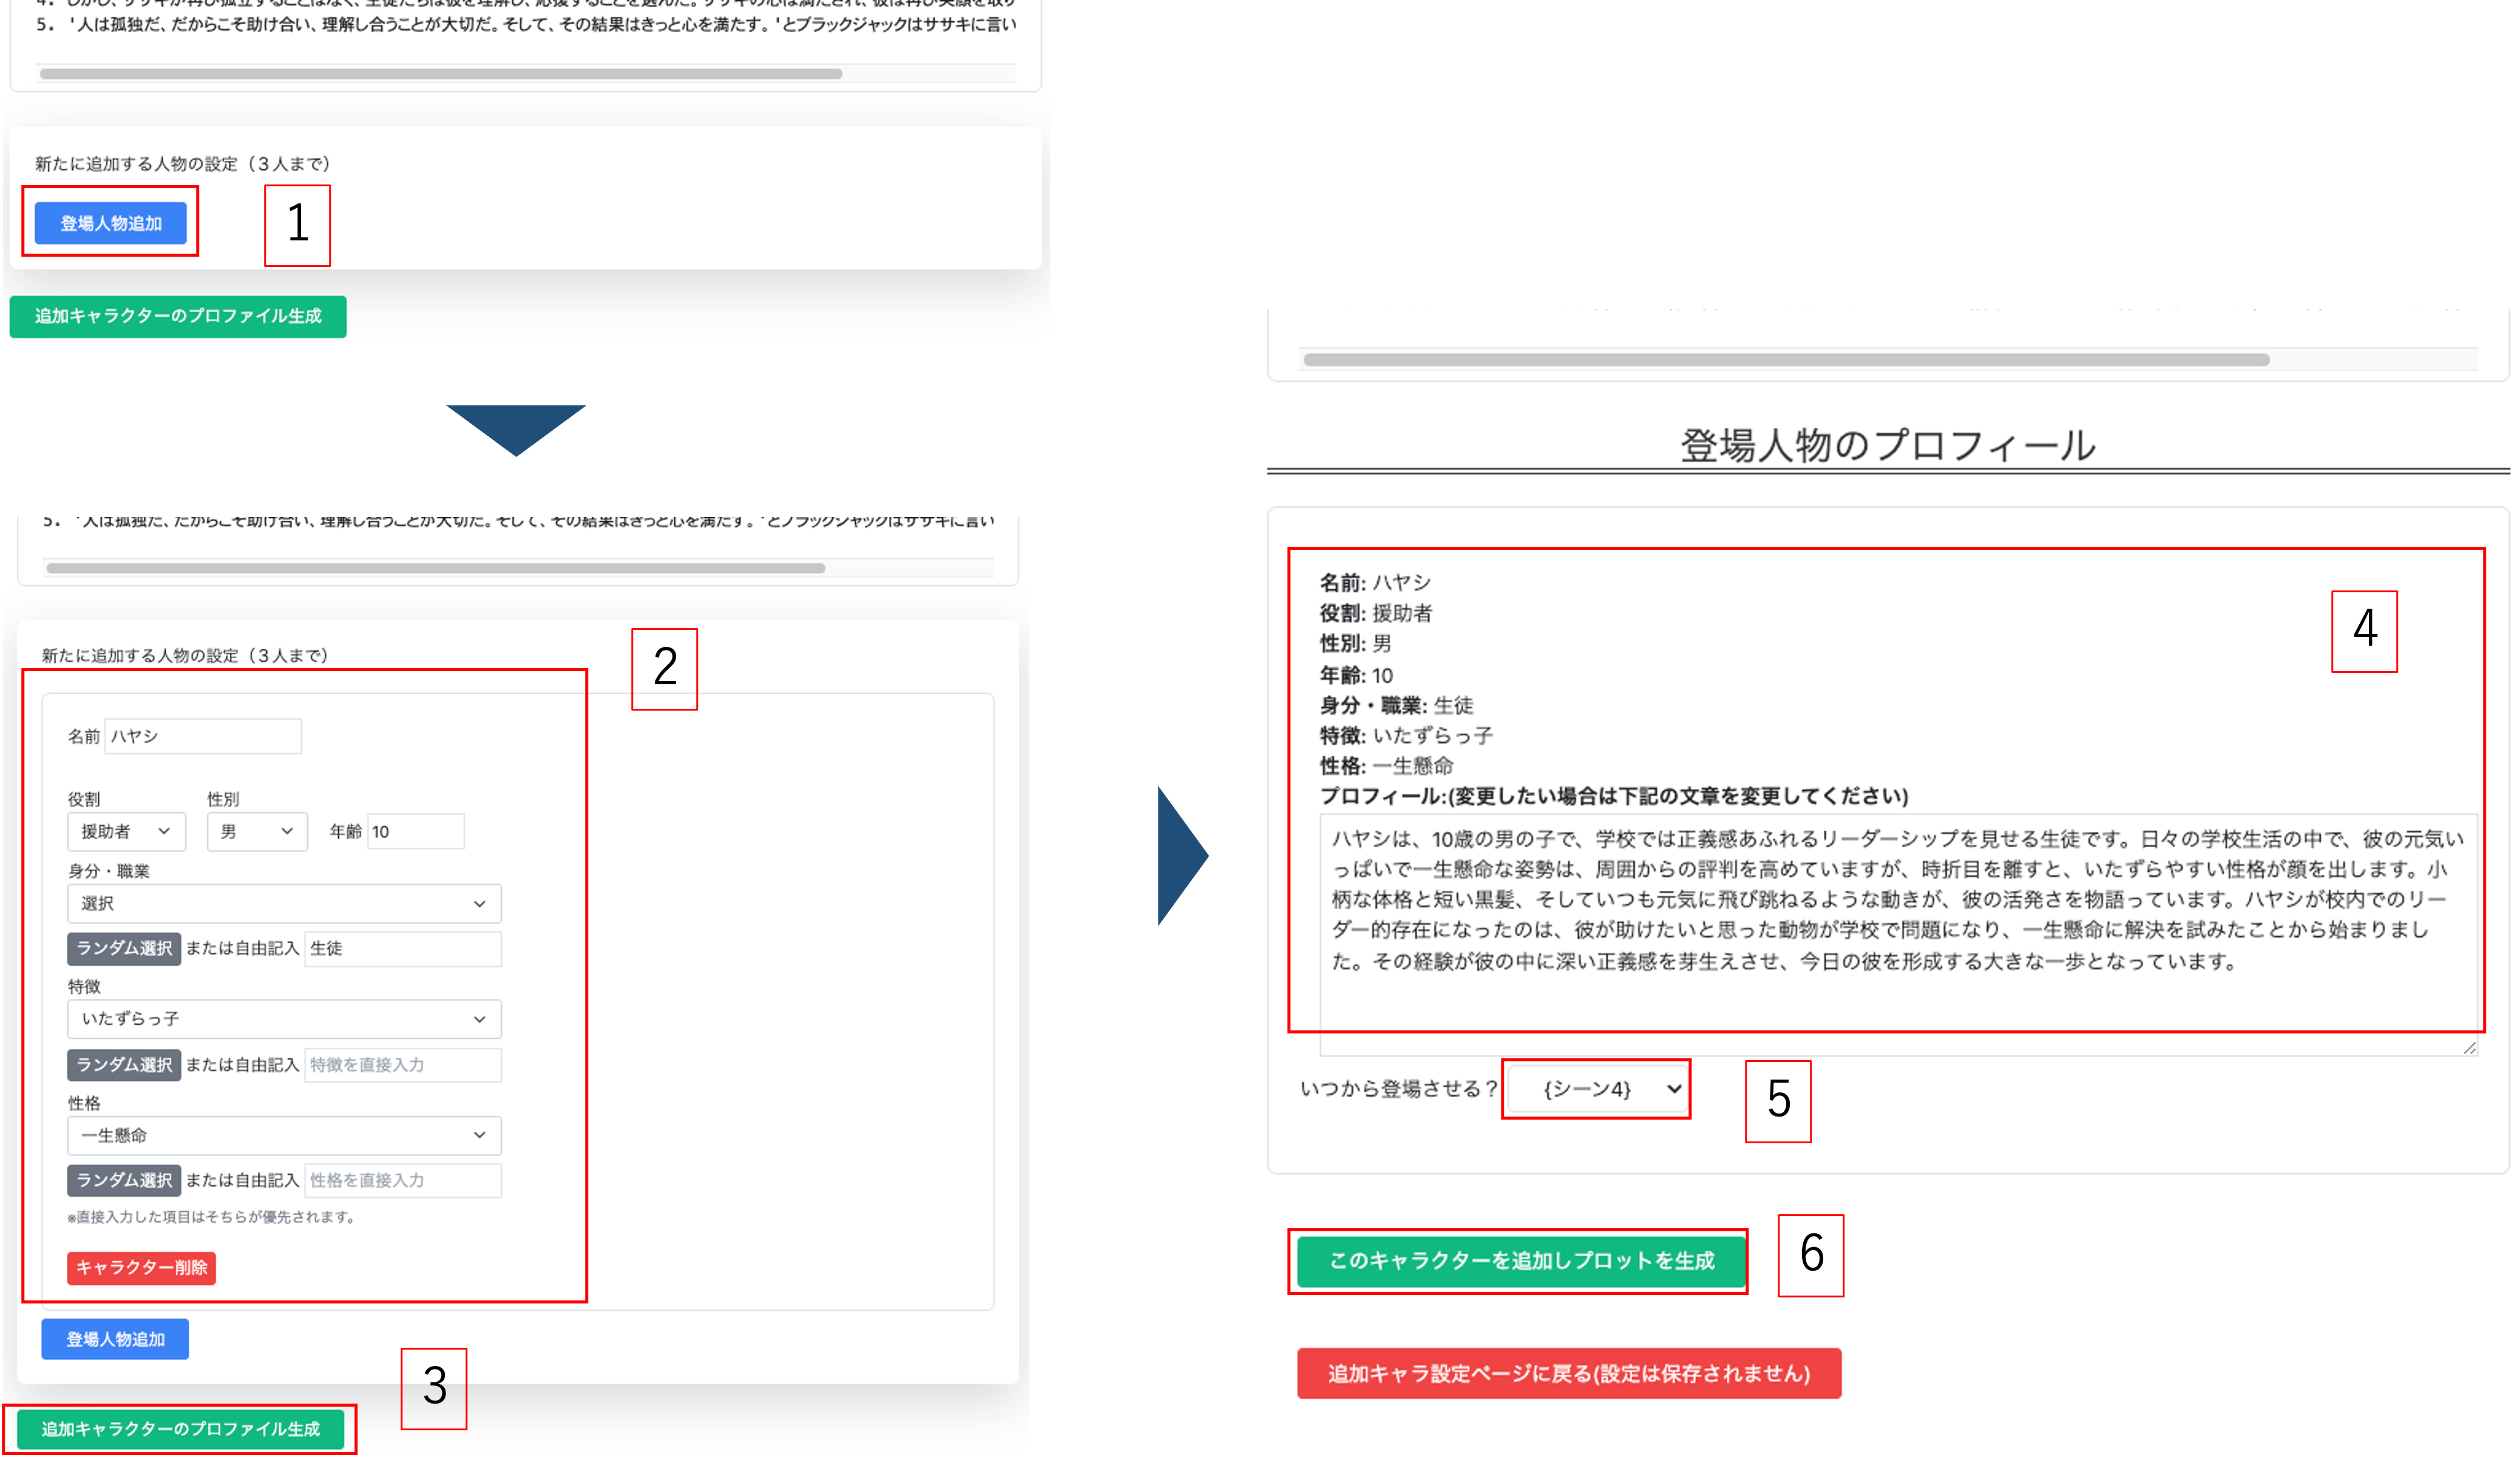
\includegraphics[width=12cm]{pict/04/add.png}
   \caption[登場人物の追加機能を実行する様子]{登場人物の追加機能を実行する様子. \small (1): 「登場人物追加」ボタンを押す. (2): 登場人物の名前等属性を入力するコンテナが展開. 名前等属性を設定する. (3): 「追加キャラクターのプロファイル生成」を押す. (4): LLMを介してプロフィールが生成される. ユーザー自身の手で編集することも可能. (5): 新規キャラクターをどのシーンから登場させるかを選択する. (6): 「このキャラクターを追加しプロットを生成」を押すと, 新規キャラクターが登場するプロットが生成され, 新旧プロットの比較画面へと遷移する.}
   \label{add}
   \end{center}
\end{figure}

\subsection{登場人物の役割変更}
\label{subsec: change_role}
この機能は, 既存のプロットに登場する人物の役割等属性やプロフィール情報を変更することができる機能である. Propp\cite{Propp68}が示したように, 登場人物が持つ行動領域はその役割に応じて異なるため, 物語における役割の重要性は大きい. 加えて, 詳細なプロフィール情報は, 物語創作におけるLLMの制御において重要な要素の一つとされている\cite{mirowski23}. これらの重要な要素を簡便に設定し直し, 役割が変更された場合に生じるプロットの変化の一例を容易に獲得することができるこの機能は創作支援に役立つものと考えられる.

この機能を操作している様子を図\ref{change_role}に示す. 図\ref{change_role}に示した通り, 既存のプロットに登場する人物の役割等属性やプロフィール情報の変更はコンテナ内に表示された情報を変更することで容易に行うことができる. さらにこの機能では, 登場人物の設定の変更をどのシーンから反映させるか選択することができ, 登場人物の行動を細かく制御することができる. このことにより, 物語に複雑性を持たせる裏切りや意外性を含めるような工夫を施す試みが可能となり, これは創作支援に役立つものと考えられる.


\begin{figure}[H]
   \begin{center}
   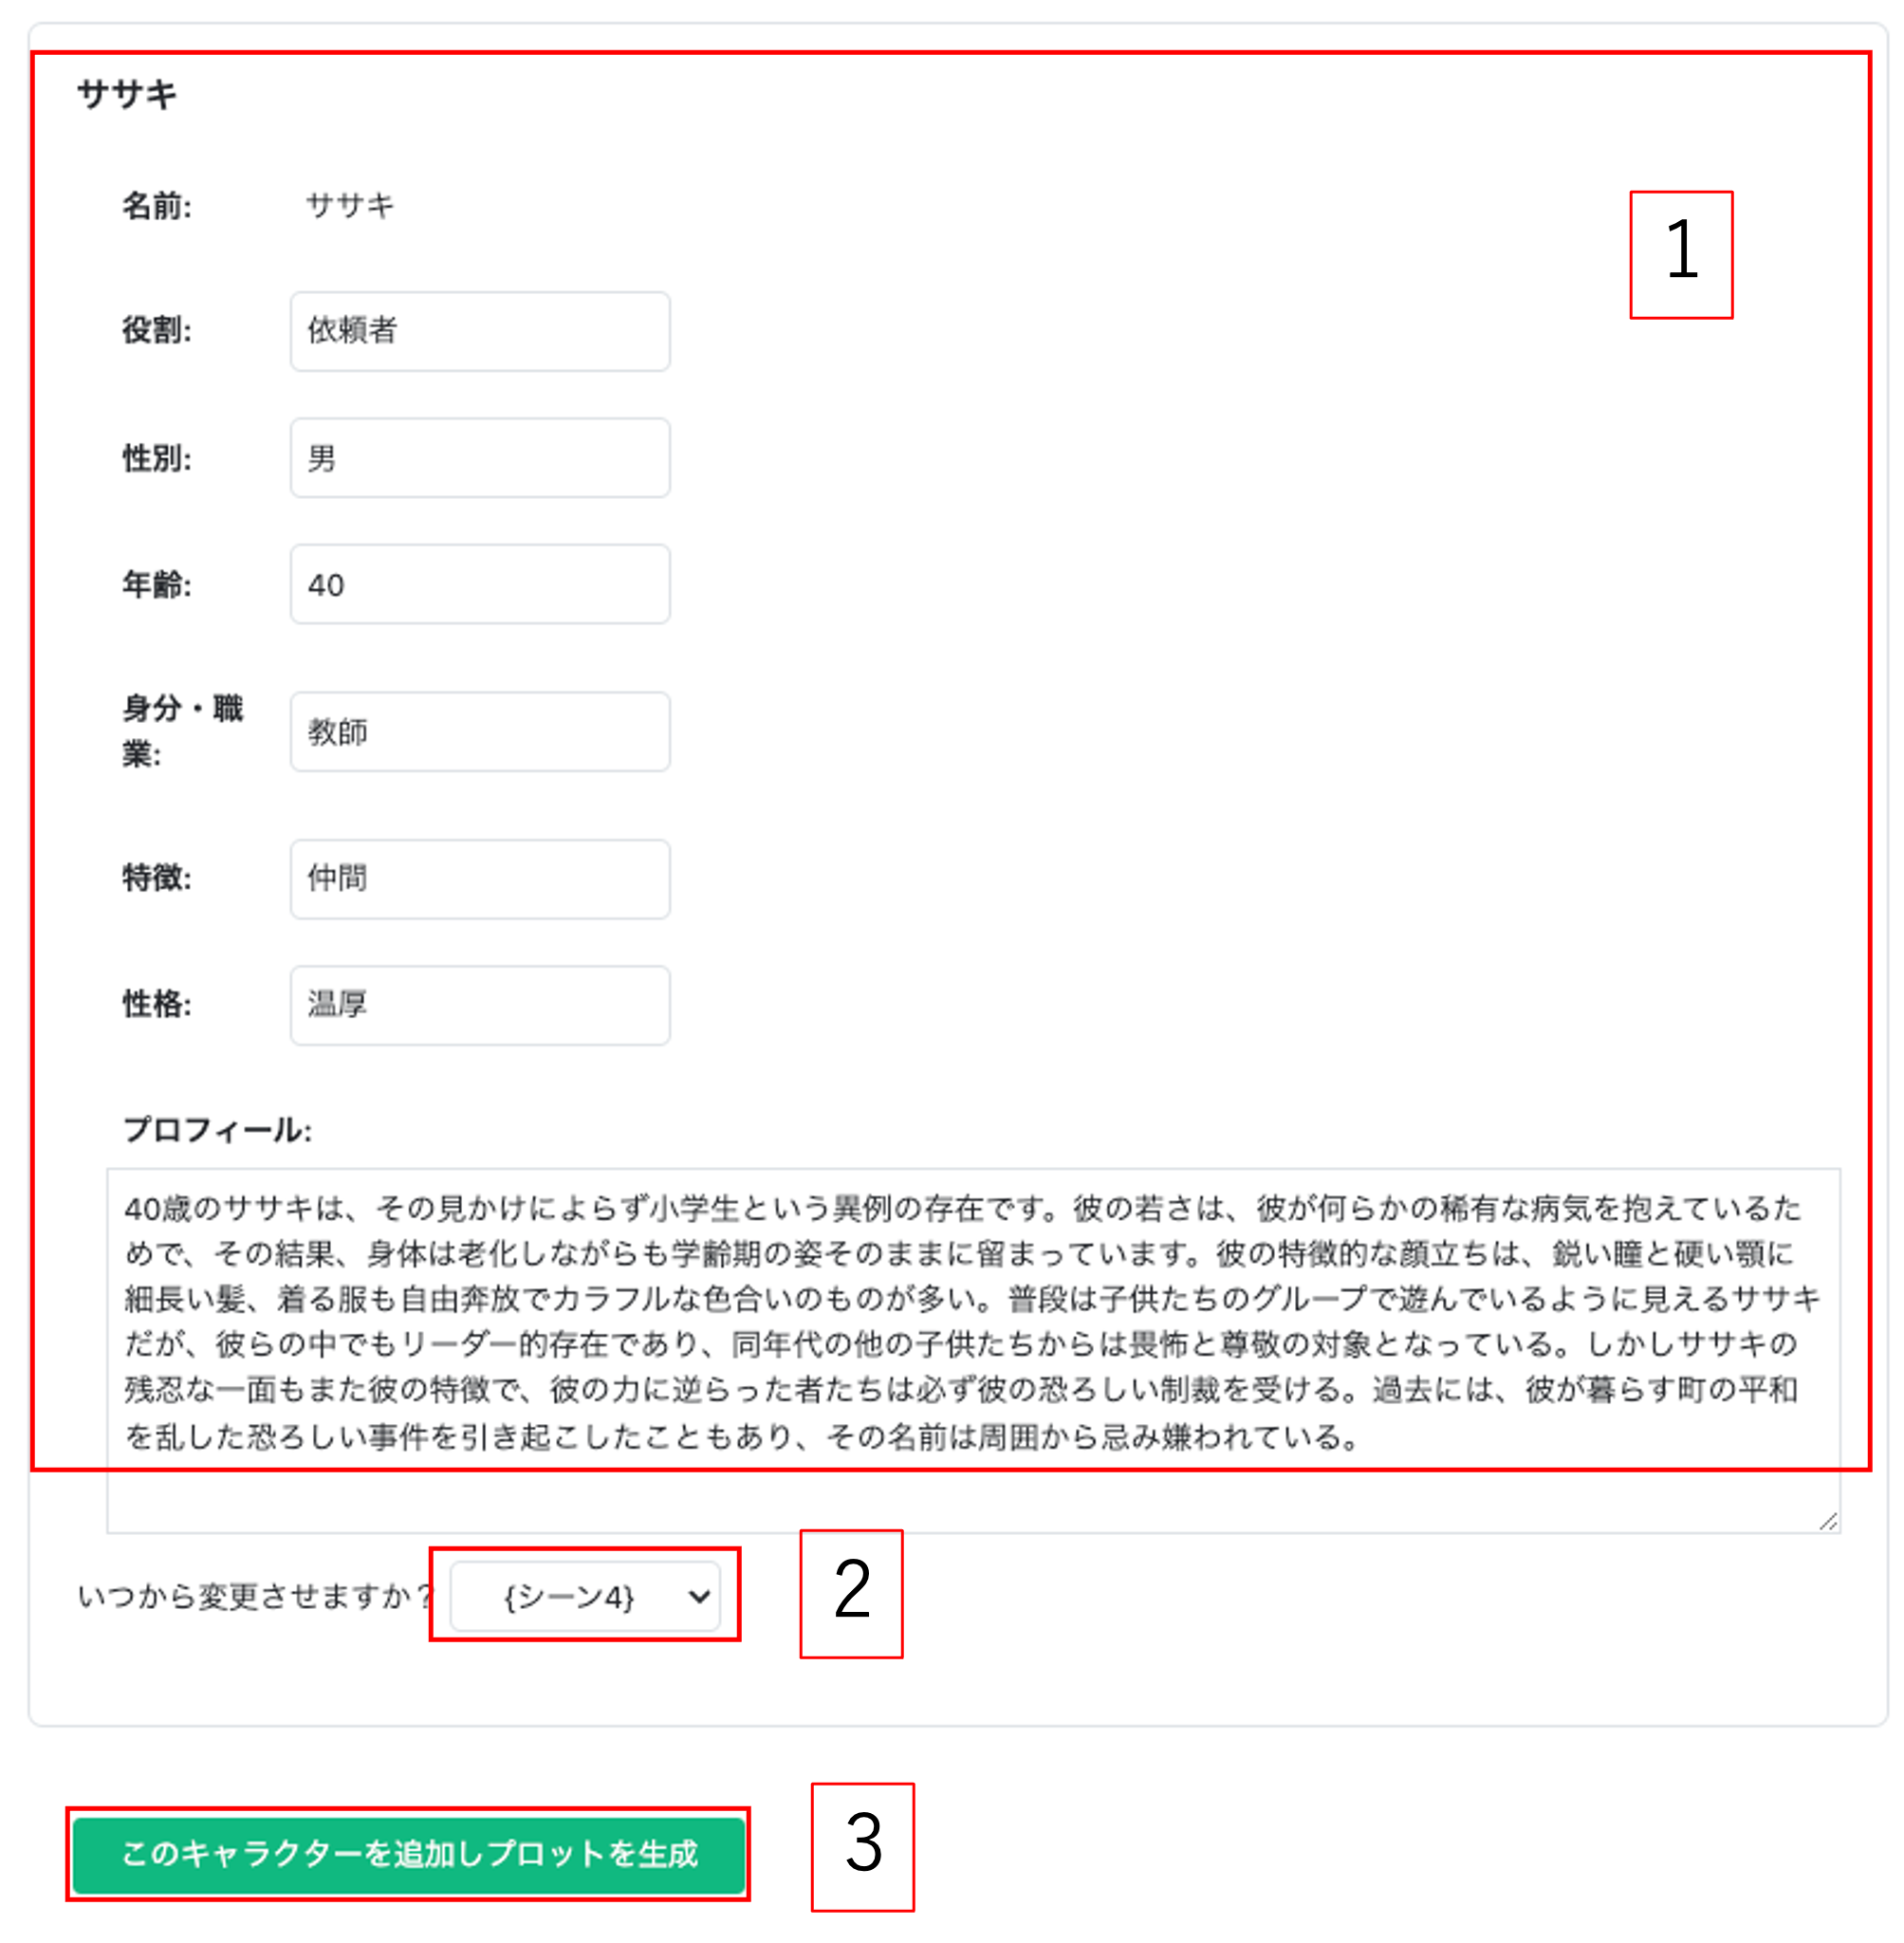
\includegraphics[width=10cm]{pict/04/change_role.png}
   \caption[登場人物の役割変更機能を実行する様子]{登場人物の役割変更機能を実行する様子. \small (1): 登場人物の属性等の変更を行う. (2): どのシーンからその設定を反映させるかを選択する. (3): 「このキャラクターを追加しプロットを生成」を押すと, 新たに設定した内容が反映されるよう書き換えられたプロットが生成され, 新旧プロットの比較画面へと遷移する.}
   \label{change_role}
   \end{center}
\end{figure}

\subsection{プロットの部分修正}
\label{subsec: modify}
この機能は, 既存のプロットの一部を修正することができる機能である. この機能を用いることで, 既存のプロットの一部を修正した場合に生じるプロットの変化の一例を容易に獲得することができ, これは創作支援に役立つものと考えられる.

この機能を操作している様子を図\ref{modify}に示す. 図\ref{modify}に示した通り, 既存のプロットの一部分の修正は, シーンの選択とその内容の入力により簡単に行うことができる. 

\begin{figure}[H]
   \begin{center}
   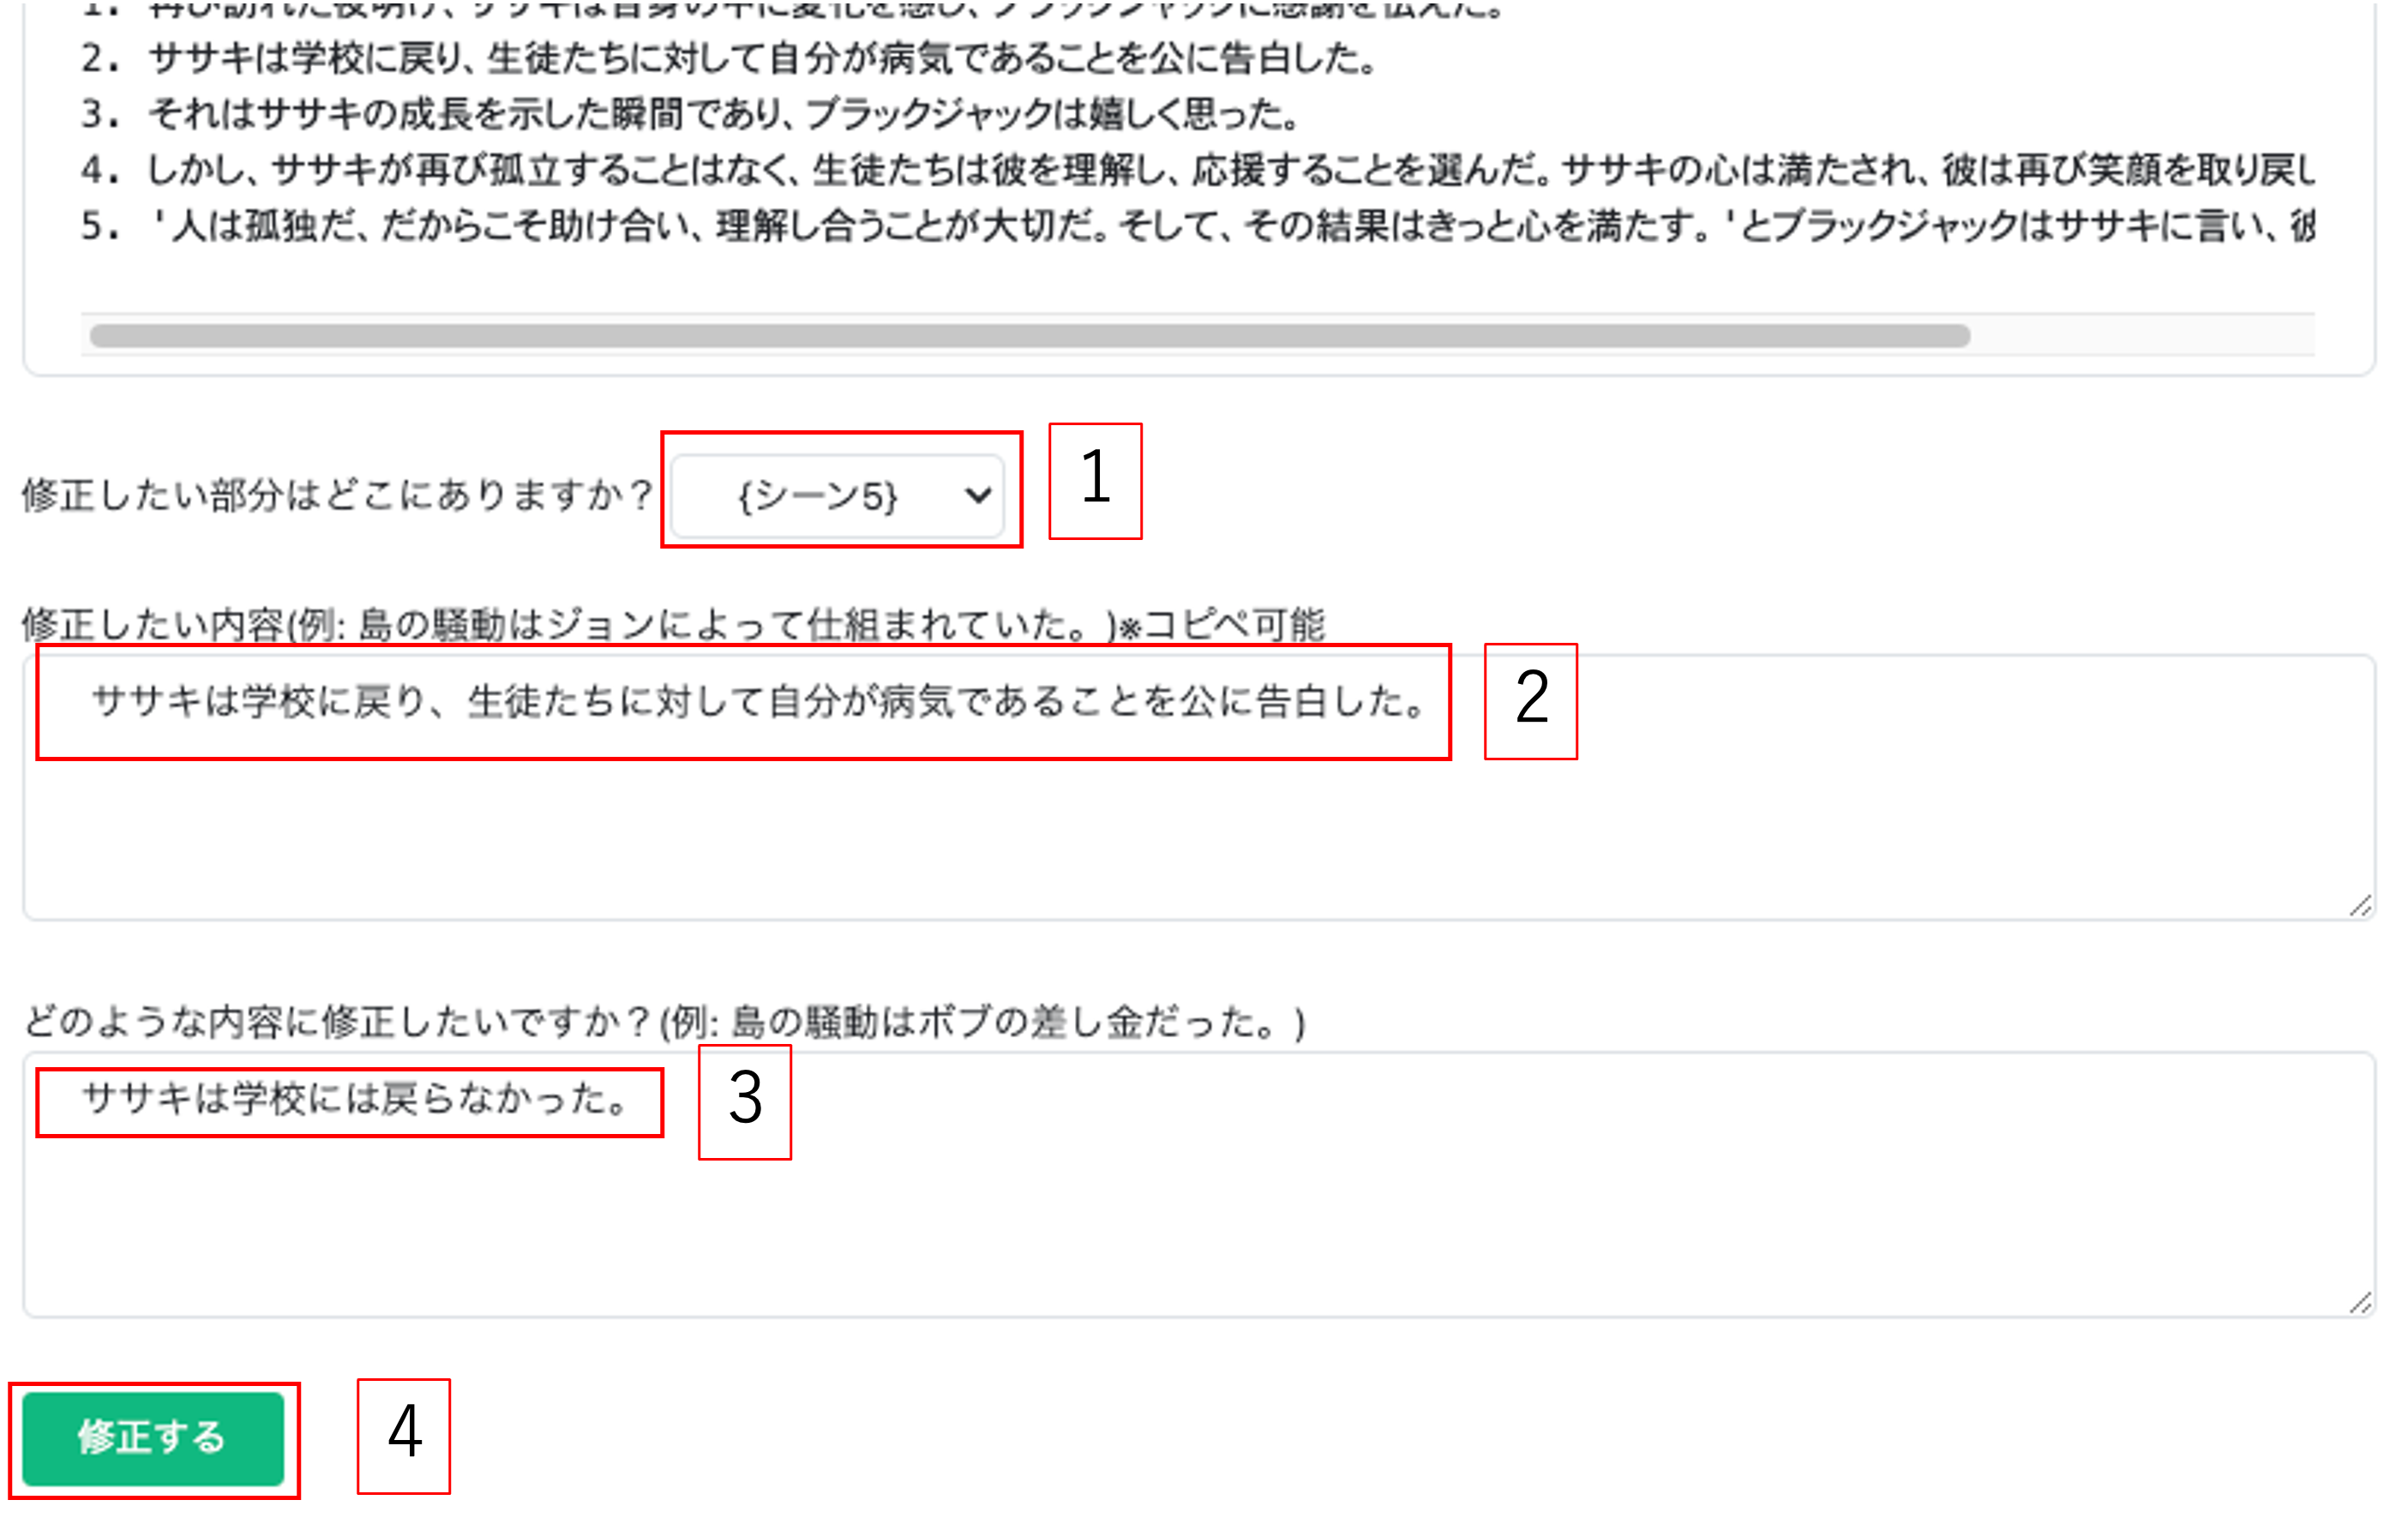
\includegraphics[width=10cm]{pict/04/modify.png}
   \caption[プロットの部分修正機能を実行する様子]{プロットの部分修正機能を実行する様子. \small (1): 修正したい内容があるシーンを選択する. (2): 修正したい内容をテキストエリアに入力する. (3): どのように修正したいかをテキストエリアに入力する. (4): 「修正する」ボタンを押すと, 修正した内容が反映されるよう書き換えられたプロットが生成され, 新旧プロットの比較画面へと遷移する.}
   \label{modify}
   \end{center}
\end{figure}

\subsection{不自然な日本語の修正}
\label{subsec: modify_japanese}
この機能は, 既存のプロットに含まれる不自然な日本語を修正することができる機能である. 近年のLLMの性能は極めて高く, 特にGPT-4はさまざまなベンチマークで優位な成績を収めている. しかしながらその出力は常に完璧なものではなく, 人間が読んで不自然だと感じるものも存在する. この機能を用いることで, 既存のプロットに含まれる不自然な日本語を修正させ, その上でプロットとしてうまく成立するよう既存のプロットを書き直させることができ, この機能はLLMとのストーリー共創において役立つものと考えられる.

この機能を操作している様子を図\ref{modify_j}に示す. 図\ref{modify_j}に示した通り, 操作は不自然だと感じる言葉がどのシーンにあるのかを選択し, その内容をコピーアンドペーストなどでテキストエリアに入力するだけでよい. 容易な操作によりクリエーターの負担を軽減し, 創作を支援する.

\begin{figure}[H]
   \begin{center}
   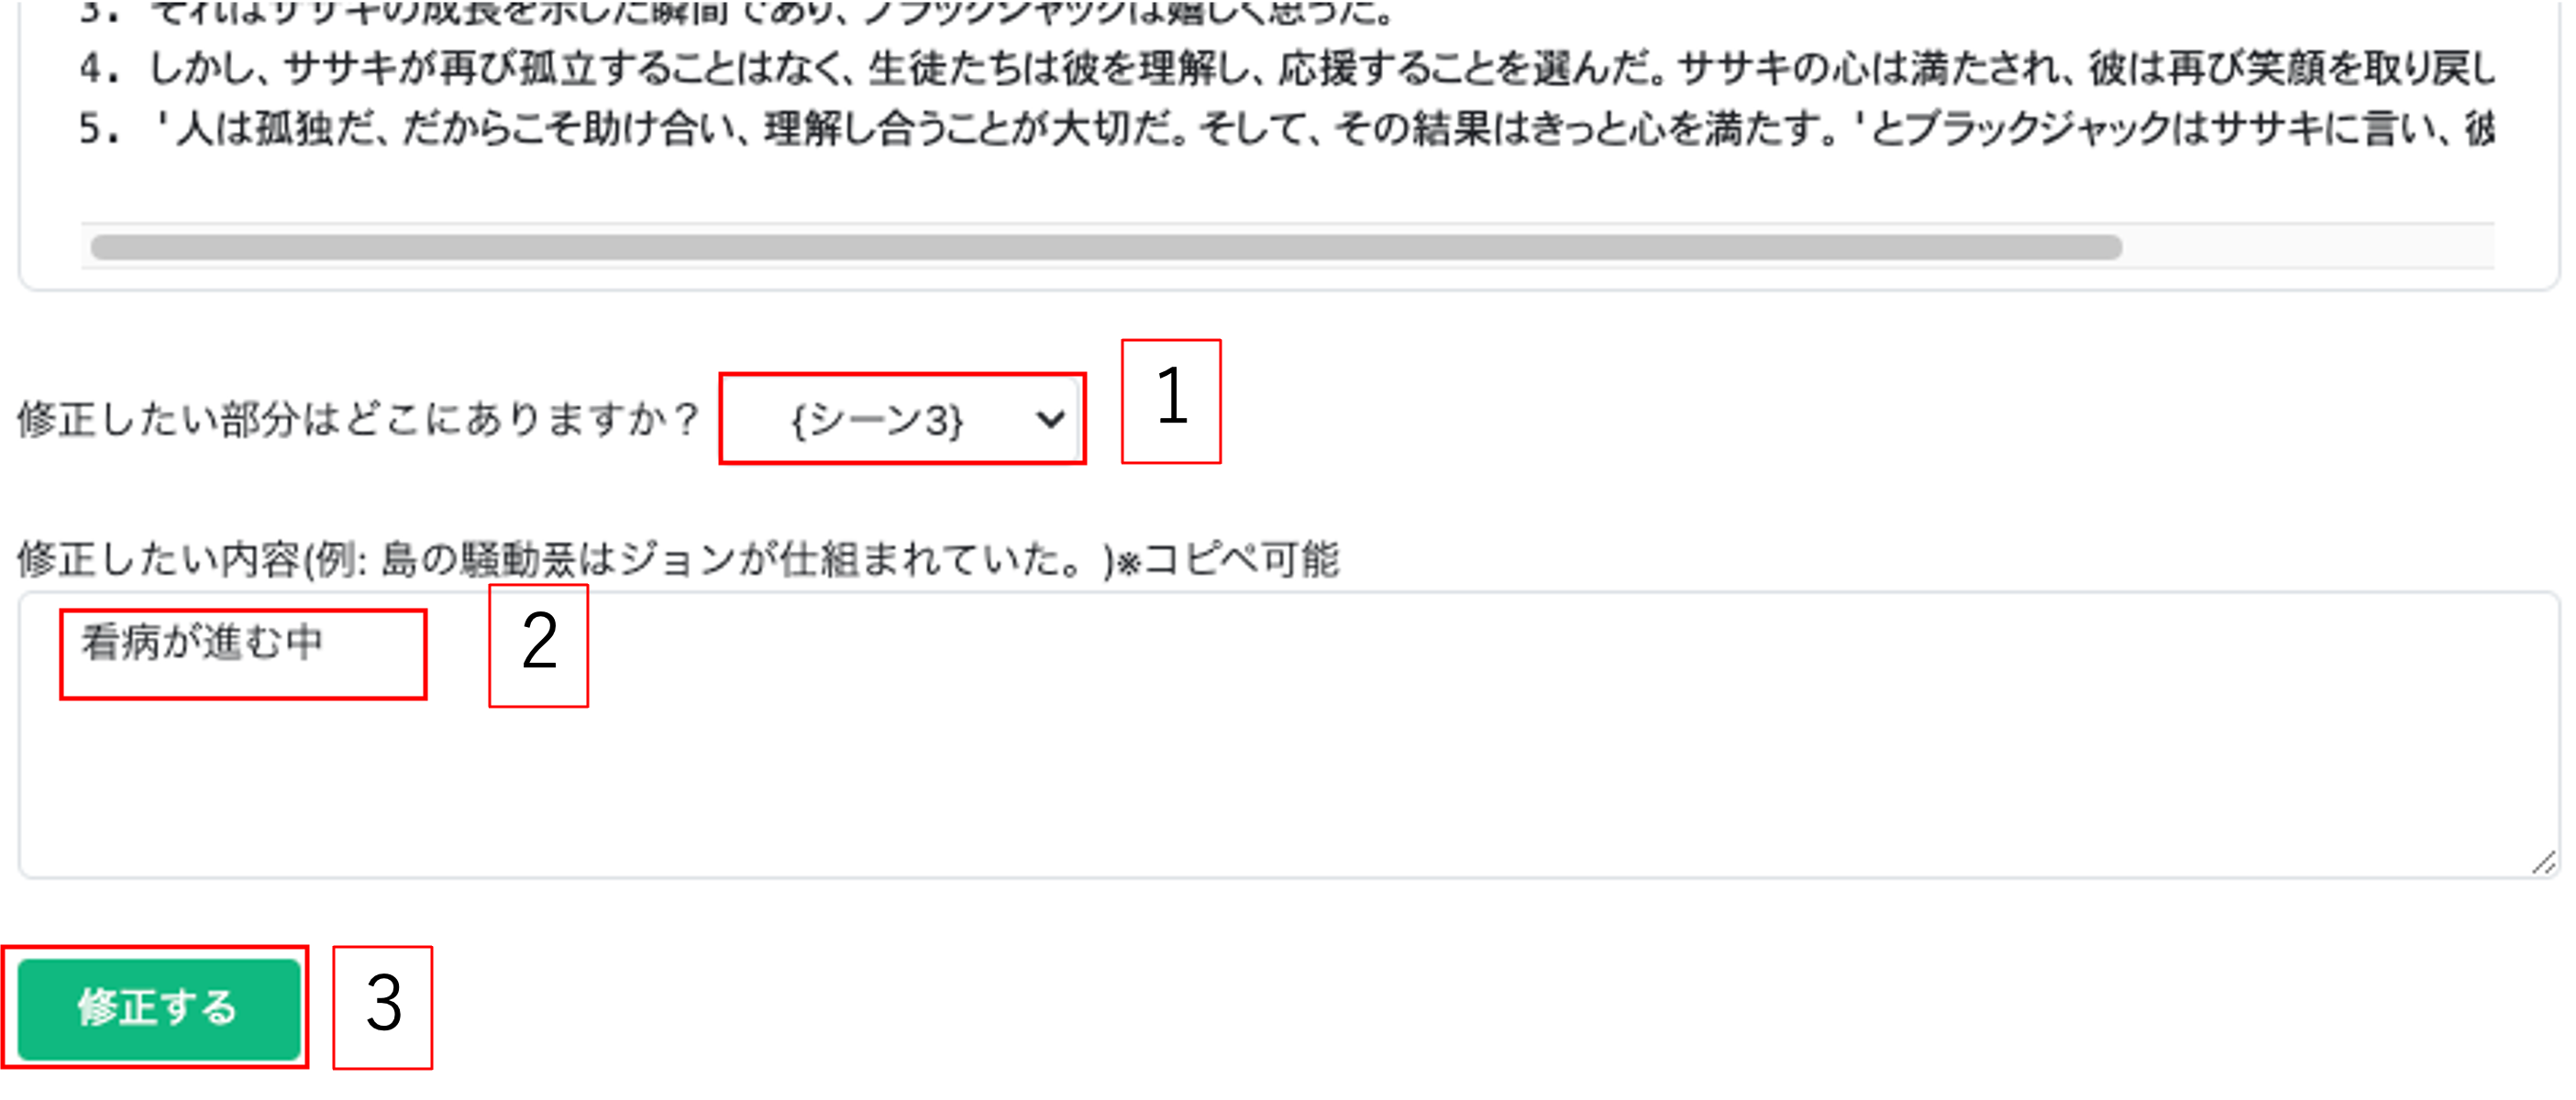
\includegraphics[width=12cm]{pict/04/modify_j.png}
   \caption[不自然な日本語の修正機能を実行する様子]{不自然な日本語の修正機能を実行する様子. \small (1): 修正したい内容があるシーンを選択する. (2): 修正したい内容をテキストエリアに入力する. (3): 「修正する」ボタンを押すと, 修正した内容が反映されるよう書き換えられたプロットが生成され, 新旧プロットの比較画面へと遷移する.}
   \label{modify_j}
   \end{center}
\end{figure}

\subsection{プロット1シーンの起承転結への分割}
\label{subsec: divide}
この機能は, 既存のプロットの中の一つのシーンを起承転結に分割することができる機能である.

物語の構成としてよく知られる起承転結の枠組みであるが, 作品性の高い物語の中には, 物語全体として起承転結の枠組みを持ちながらその内部にも細かな起承転結を含むものがある. この機能は, 物語の内部に部分的な起承転結構造を持たせるようプロットを書き換え生成させることができる機能であり, 物語の作品性の向上を提供する. プロットの長さを確保する面においても役に立ち, この機能はストーリークリエーターの創作支援に有益なものであると考える. 

この機能を操作している様子を図\ref{divide}に示す. 操作は, 図\ref{divide}に示す通りで, 分割したいシーンが入力されているコンテナ上で操作する. 既存の内容のまま分割したければそのまま「このシーンを起承転結に分割する」ボタンを押すだけでよく, 既存の内容を自身の手で編集してから起承転結に分割させることもできる. 

上述したように, 容易な操作で物語に重曹性を持たせるもたせることを試みられるこの機能は, 創作支援に役立つものと考えられる.

\begin{figure}[H]
   \begin{center}
   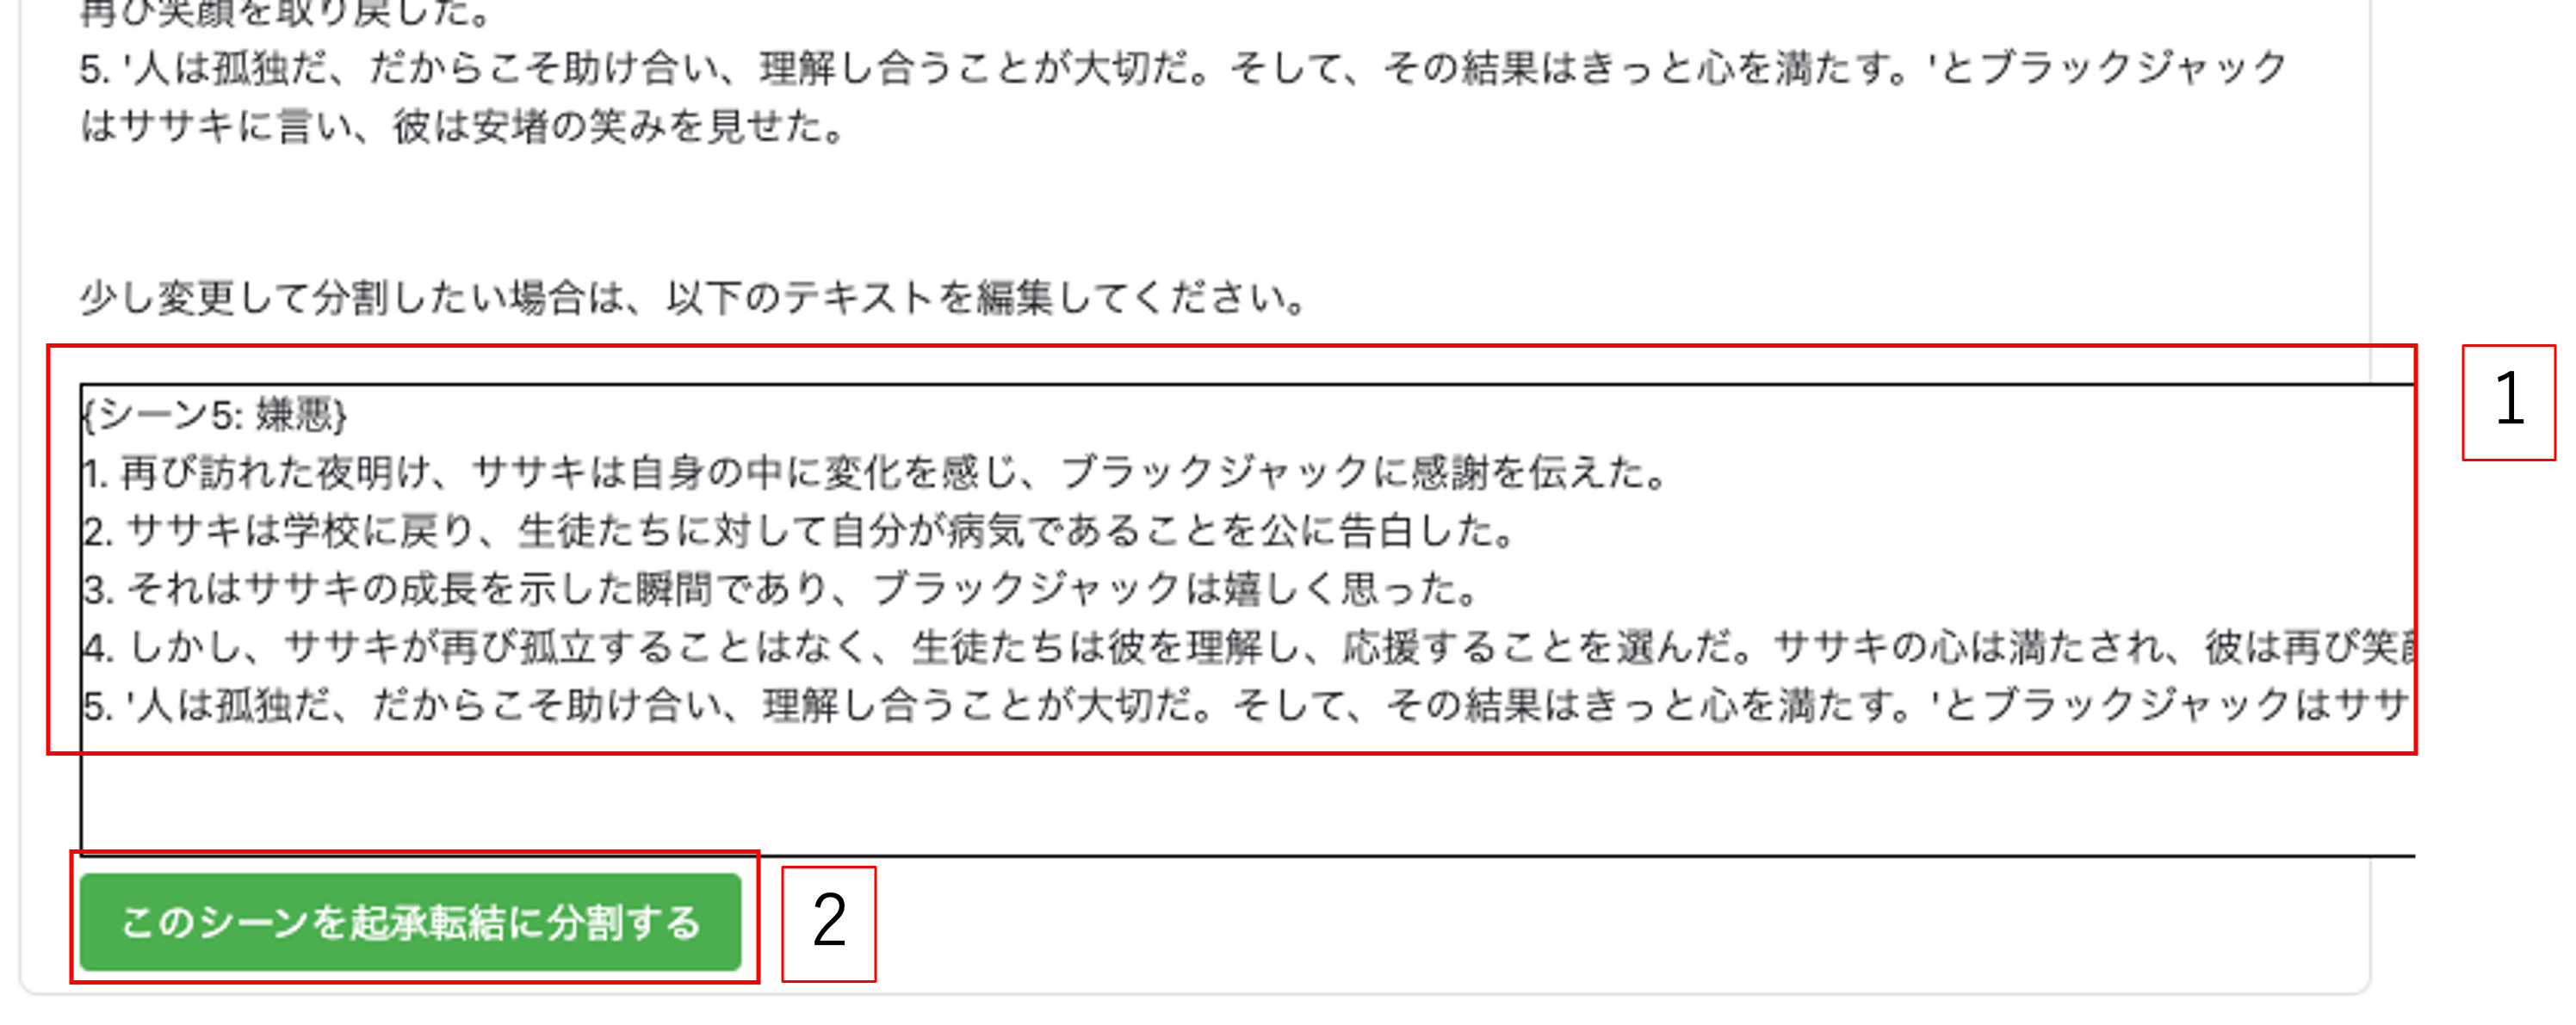
\includegraphics[width=12cm]{pict/04/divide.png}
   \caption[プロット1シーンの起承転結への分割機能を実行する様子]{プロット1シーンの起承転結への分割機能を実行する様子. \small (1): 分割したいシーンが入力されたテキストエリアにおいて, 修正するべきことがあればテキストを編集する. (2): 「このシーンを起承転結に分割する」ボタンを押すと, 選択したシーンが起承転結に分割されるよう書き換えられたプロットが生成され, 新旧プロットの比較画面へと遷移する.}
   \label{divide}
   \end{center}
\end{figure}

\subsection{手作業での編集}
\label{subsec: manual}
この機能は, 既存のプロットを手作業で編集するための機能である. これまでに示した, ユーザーの入力を元にLLMを制御し, 既存のプロットを書き換え生成させる機能とは
大きく異なり, この機能でLLM介すことはない. この機能の目的はこれまでのプロット創作の過程において受けた刺激を元に想起されたアイデアなどを自分自身の手でプロットに書き込めるようにすることである. 本システム自体の目的が, ストーリークリエーターの創作支援であり, ストーリークリエーター自身の考えや言葉を直接描くための場は必要不可欠な場であり, この機能はその場を提供するものである.

この機能を操作している様子を図\ref{manual}に示す. 図\ref{manual}に示した通り, 操作は非常に単純で, ただテキストエリアを編集すればよい. 操作は画面上部に示されている既存プロットを確認しながら行うことができる.

\begin{figure}[H]
   \begin{center}
   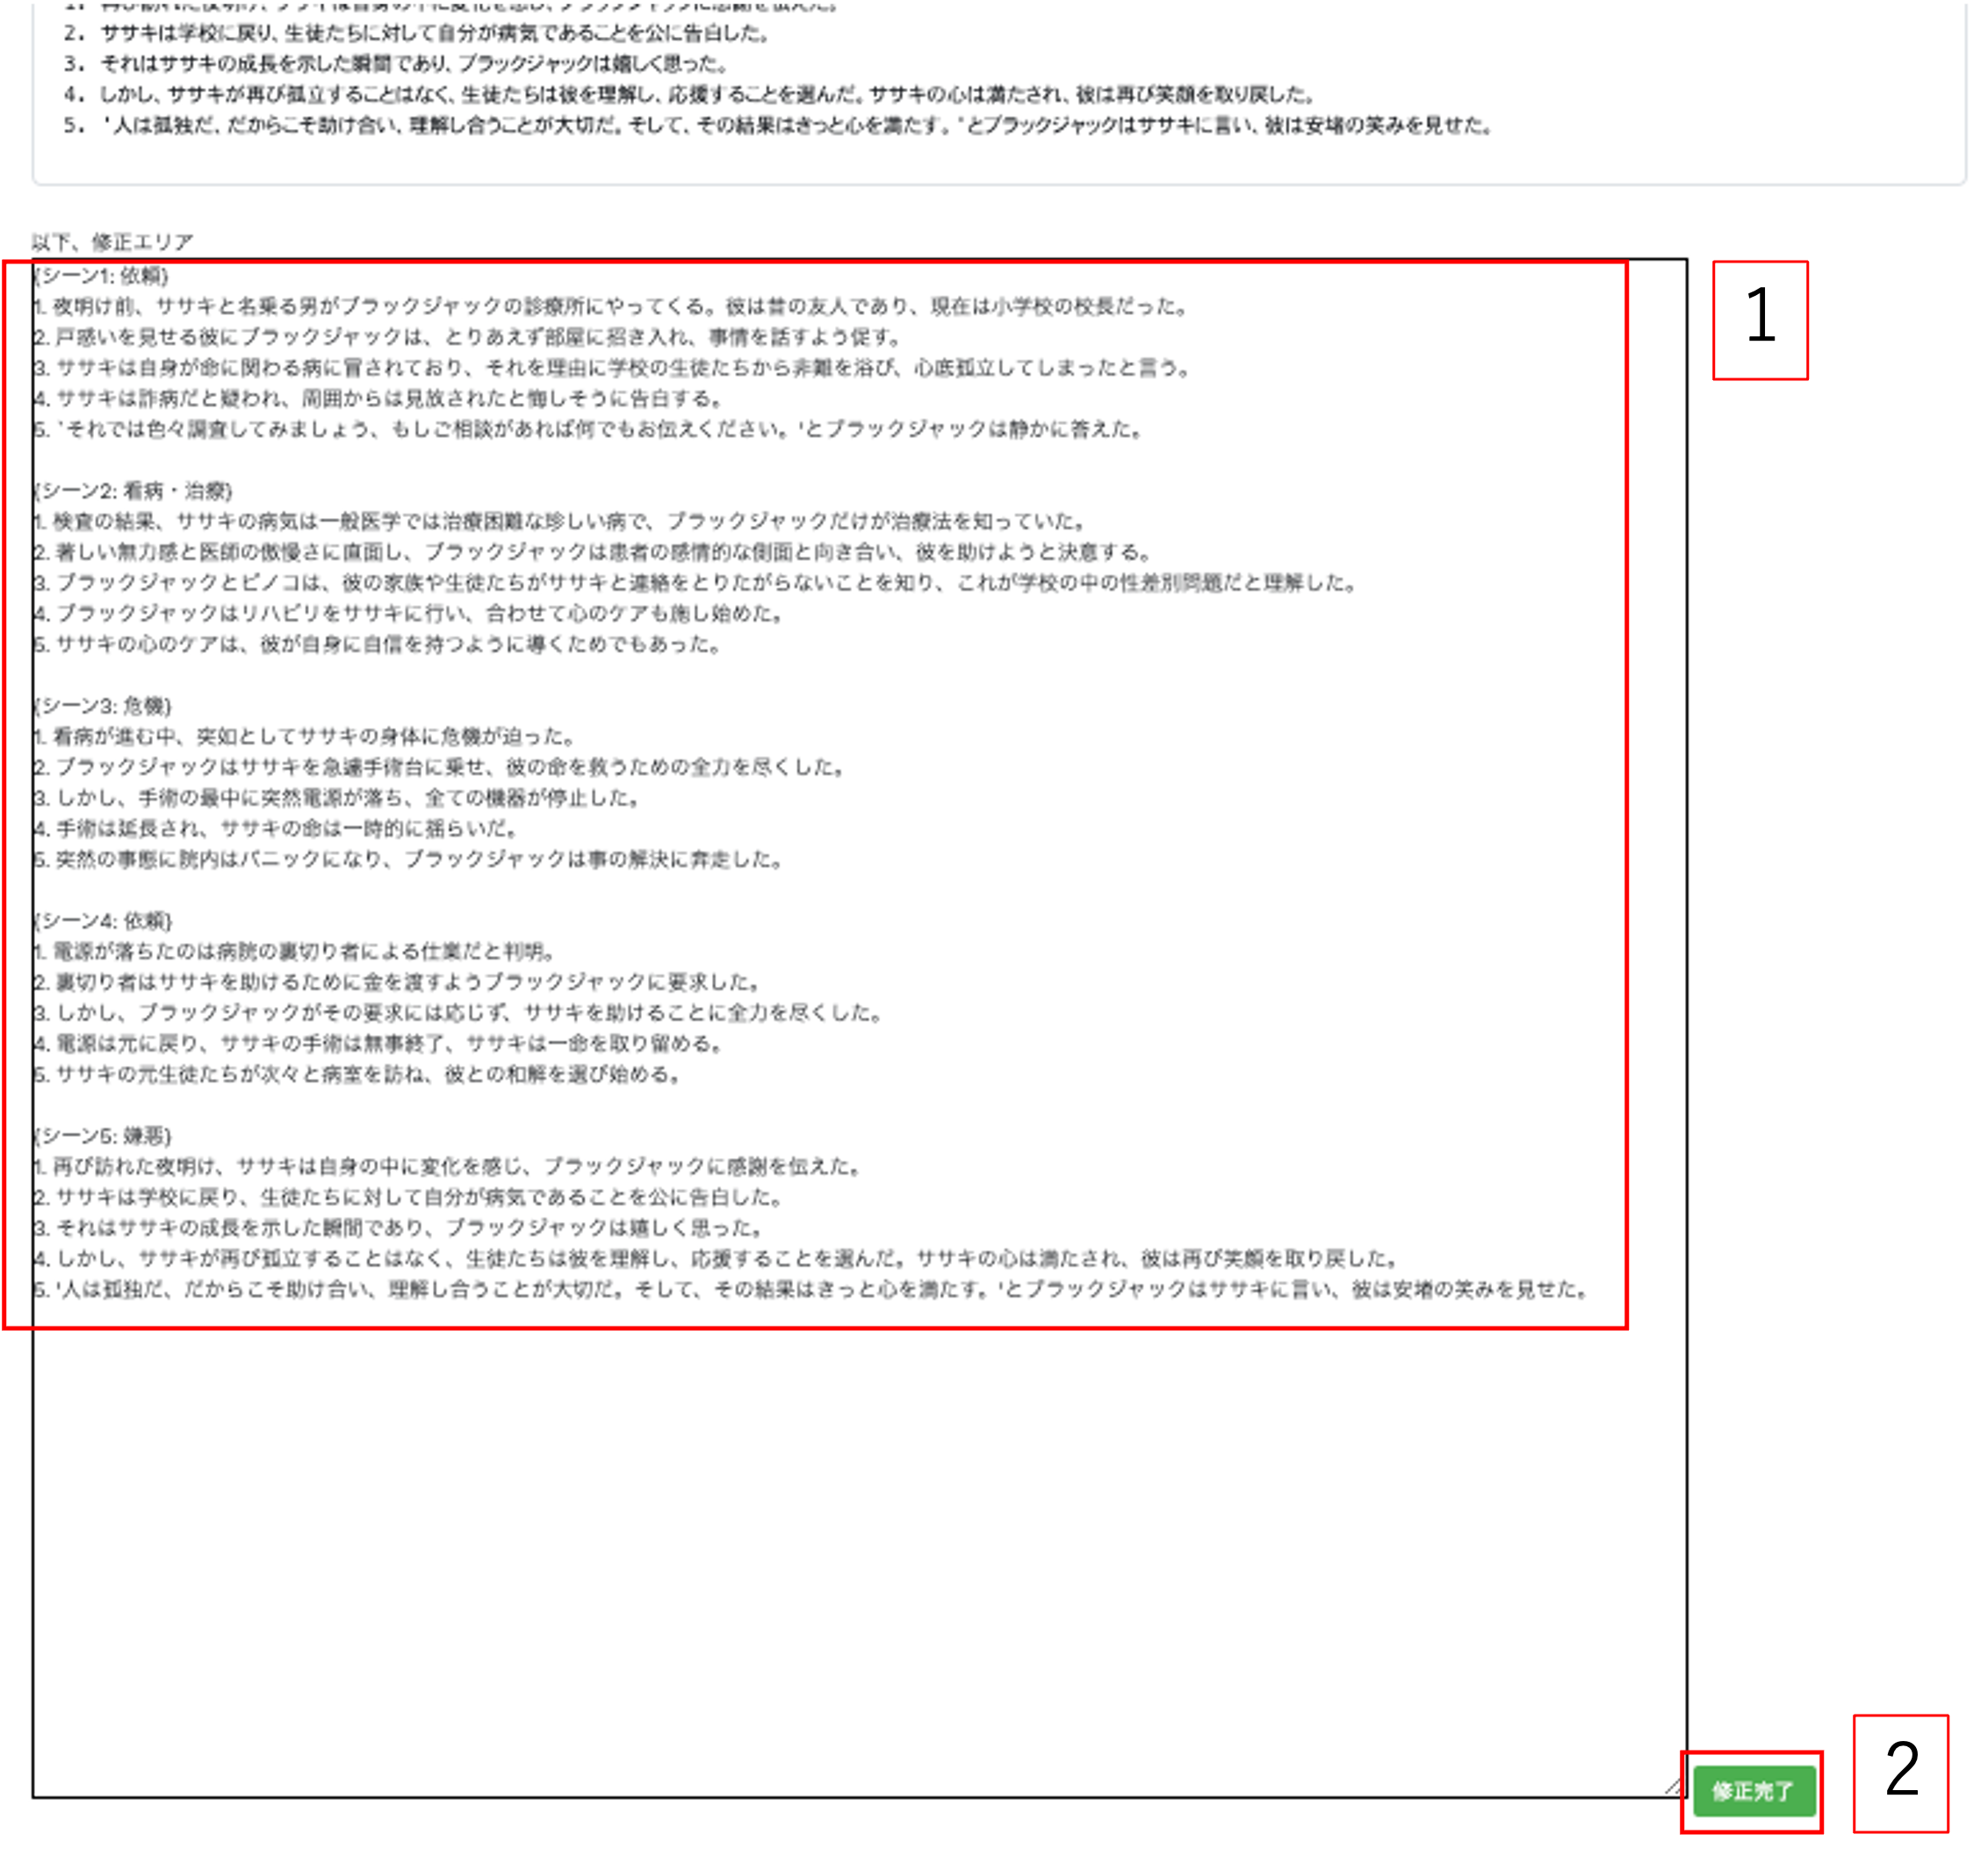
\includegraphics[width=12cm]{pict/04/manual.png}
   \caption[手作業での編集機能を実行する様子]{{\small 手作業での編集機能を実行する様子. (1): 既存のプロットがデフォルトで入力されたテキストエリアでプロットの編集を行う. (2): 「修正完了」のボタンを押すと, プロットが更新される.}}
   \label{manual}
   \end{center}
\end{figure}

\section{シナリオ生成セクション}\label{sec: scenario_generation}
シナリオとは, 一般的に映画やドラマなどの脚本を指し, ト書き, 柱, 台詞からなる物語をより具体化した文章である. ト書きとは, 登場人物の動きなど, 映像として現れるあらゆるものを言葉として記す部分を指し, 柱とは時間や場所を表す部分を指す.

本システムはストーリークリエーターの創作支援として, まず第一に物語の骨格を形成するプロット制作への支援に焦点を当てている. しかしながらプロットの制作は, 物語の創作においてその一部分を担うものでしかなく, 漫画制作等においては, キャラクターの台詞や具体的な動き, 背景, 場面などの描写を含めたシナリオの制作が必要となる. プロットという骨格にそのような肉付けをしていくことで作品は完成へと向かうため, その工程における重要度や難易度も高い.

本システムは, プロット生成セクション, プロット編集セクションを経て完成させたプロットを, LLMを介してシナリオへと変換する機能を実装している. ユーザーはこの機能を用いることにより, プロットを容易な操作でシナリオへと変換でき, より完成に近いところでの作品のイメージを得ることができる. 本システムにおいて生成されるシナリオは, 柱を含まないシナリオとなるが, これは, 柱は物語の時間や場所を表すものであり, 本システムが生成するプロットには, 既に時間や場所が設定されていることと, LLMの制御において時間間隔の制御が難しいことを理由としている. 登場人物の動きや台詞を含んだシナリオは, ストーリークリエーターへの創作支援において, 十分に創作におけるイメージやヒントを与えるものになると考えられる.

物語をより具体化するプロットからシナリオを生み出す創作は高い創造性を要する. シナリオ生成機能は, このような創作活動における困難を軽減すると考えられ, ストーリー創作支援に役立つものと考えられる.

\subsection{シナリオ生成機能1}

図\ref{scenario1}に示したのは, シナリオ生成機能1を実行する様子である. 図\ref{scenario1}に示した通り, 操作は, それぞれのキャラクターの台詞に特徴の指定があれば入力することと, 「シナリオ生成」というボタンを押すことのみである. このような容易な操作によりシナリオを生成することができる機能は, ストーリークリエーターの創作支援に役立つものと考えられる.

台詞の特徴を, 例えば関西弁などと指定することで, 生成されるシナリオにおけるキャラクターの台詞回しを一定程度制御することができる. なお, 『ブラック・ジャック』においては「ピノコ」というキャラクターの台詞が非常に特徴的であると知られているが, 「ピノコ」の台詞の特徴についてはシステム上原作の台詞まわしにのとったものとなるよう工夫が施されている.

生成されたシナリオが表示される画面の様子を図\ref{scenario1_result}に示す. 図\ref{scenario1_result}のようにその結果を画面で確認することができ, ボタンを押すだけで次のセクション, 編集セクションへと移行することができる. 仮に満足のいくシナリオが生成されなかった場合, 画面上部にある戻るボタンを押すことで再度シナリオを生成する前の段階に戻ることができる.

図\ref{scenario1_result}から分かるように, 分量は各シーン15行程度出力されるようになっているが, これは本システムにおいて, 物語がすぐに収束しないよう, LLM の制御として段階的に物語が出力されるよう工夫を施すことで実現している\cite{mirowski23}.

このような工夫が施された出力結果を容易な操作で獲得することができる本システムはストーリークリエーターの創作支援に役立つものと考えられる.

この機能で生成できるシナリオの例を図\ref{scenario1_ex}に示す.

\begin{figure}[H]
   \begin{center}
   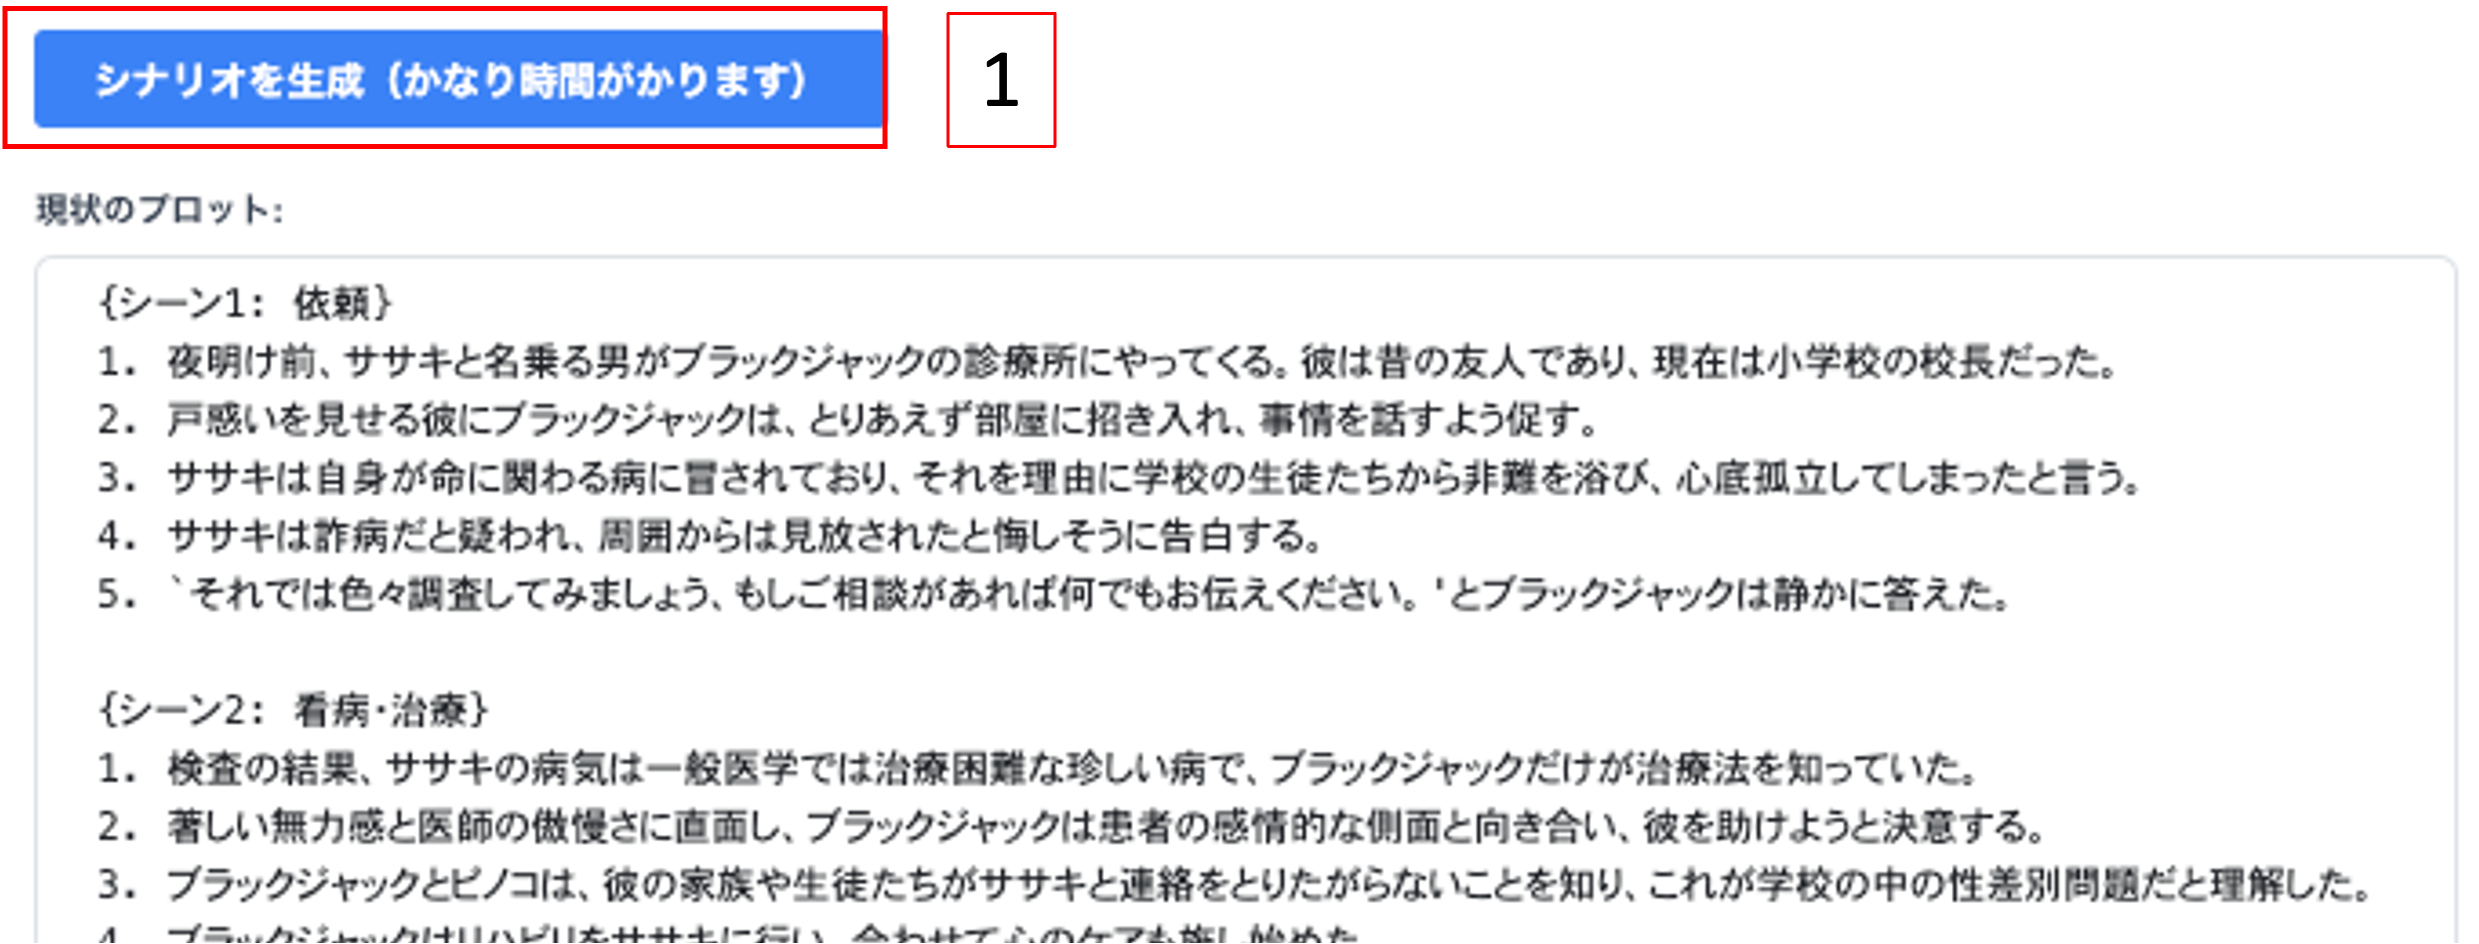
\includegraphics[width=12cm]{pict/04/scenario1.png}
   \caption[シナリオ生成機能1を実行する様子]{シナリオ生成機能1を実行する様子. \small (1): それぞれのキャラクターの台詞に特徴の指定があれば入力する. (2): 「シナリオ生成」というボタンを押すと, LLMを介しプロットからシナリオが生成される.}
   \label{scenario1}
   \end{center}
\end{figure}

\begin{figure}[H]
   \begin{center}
   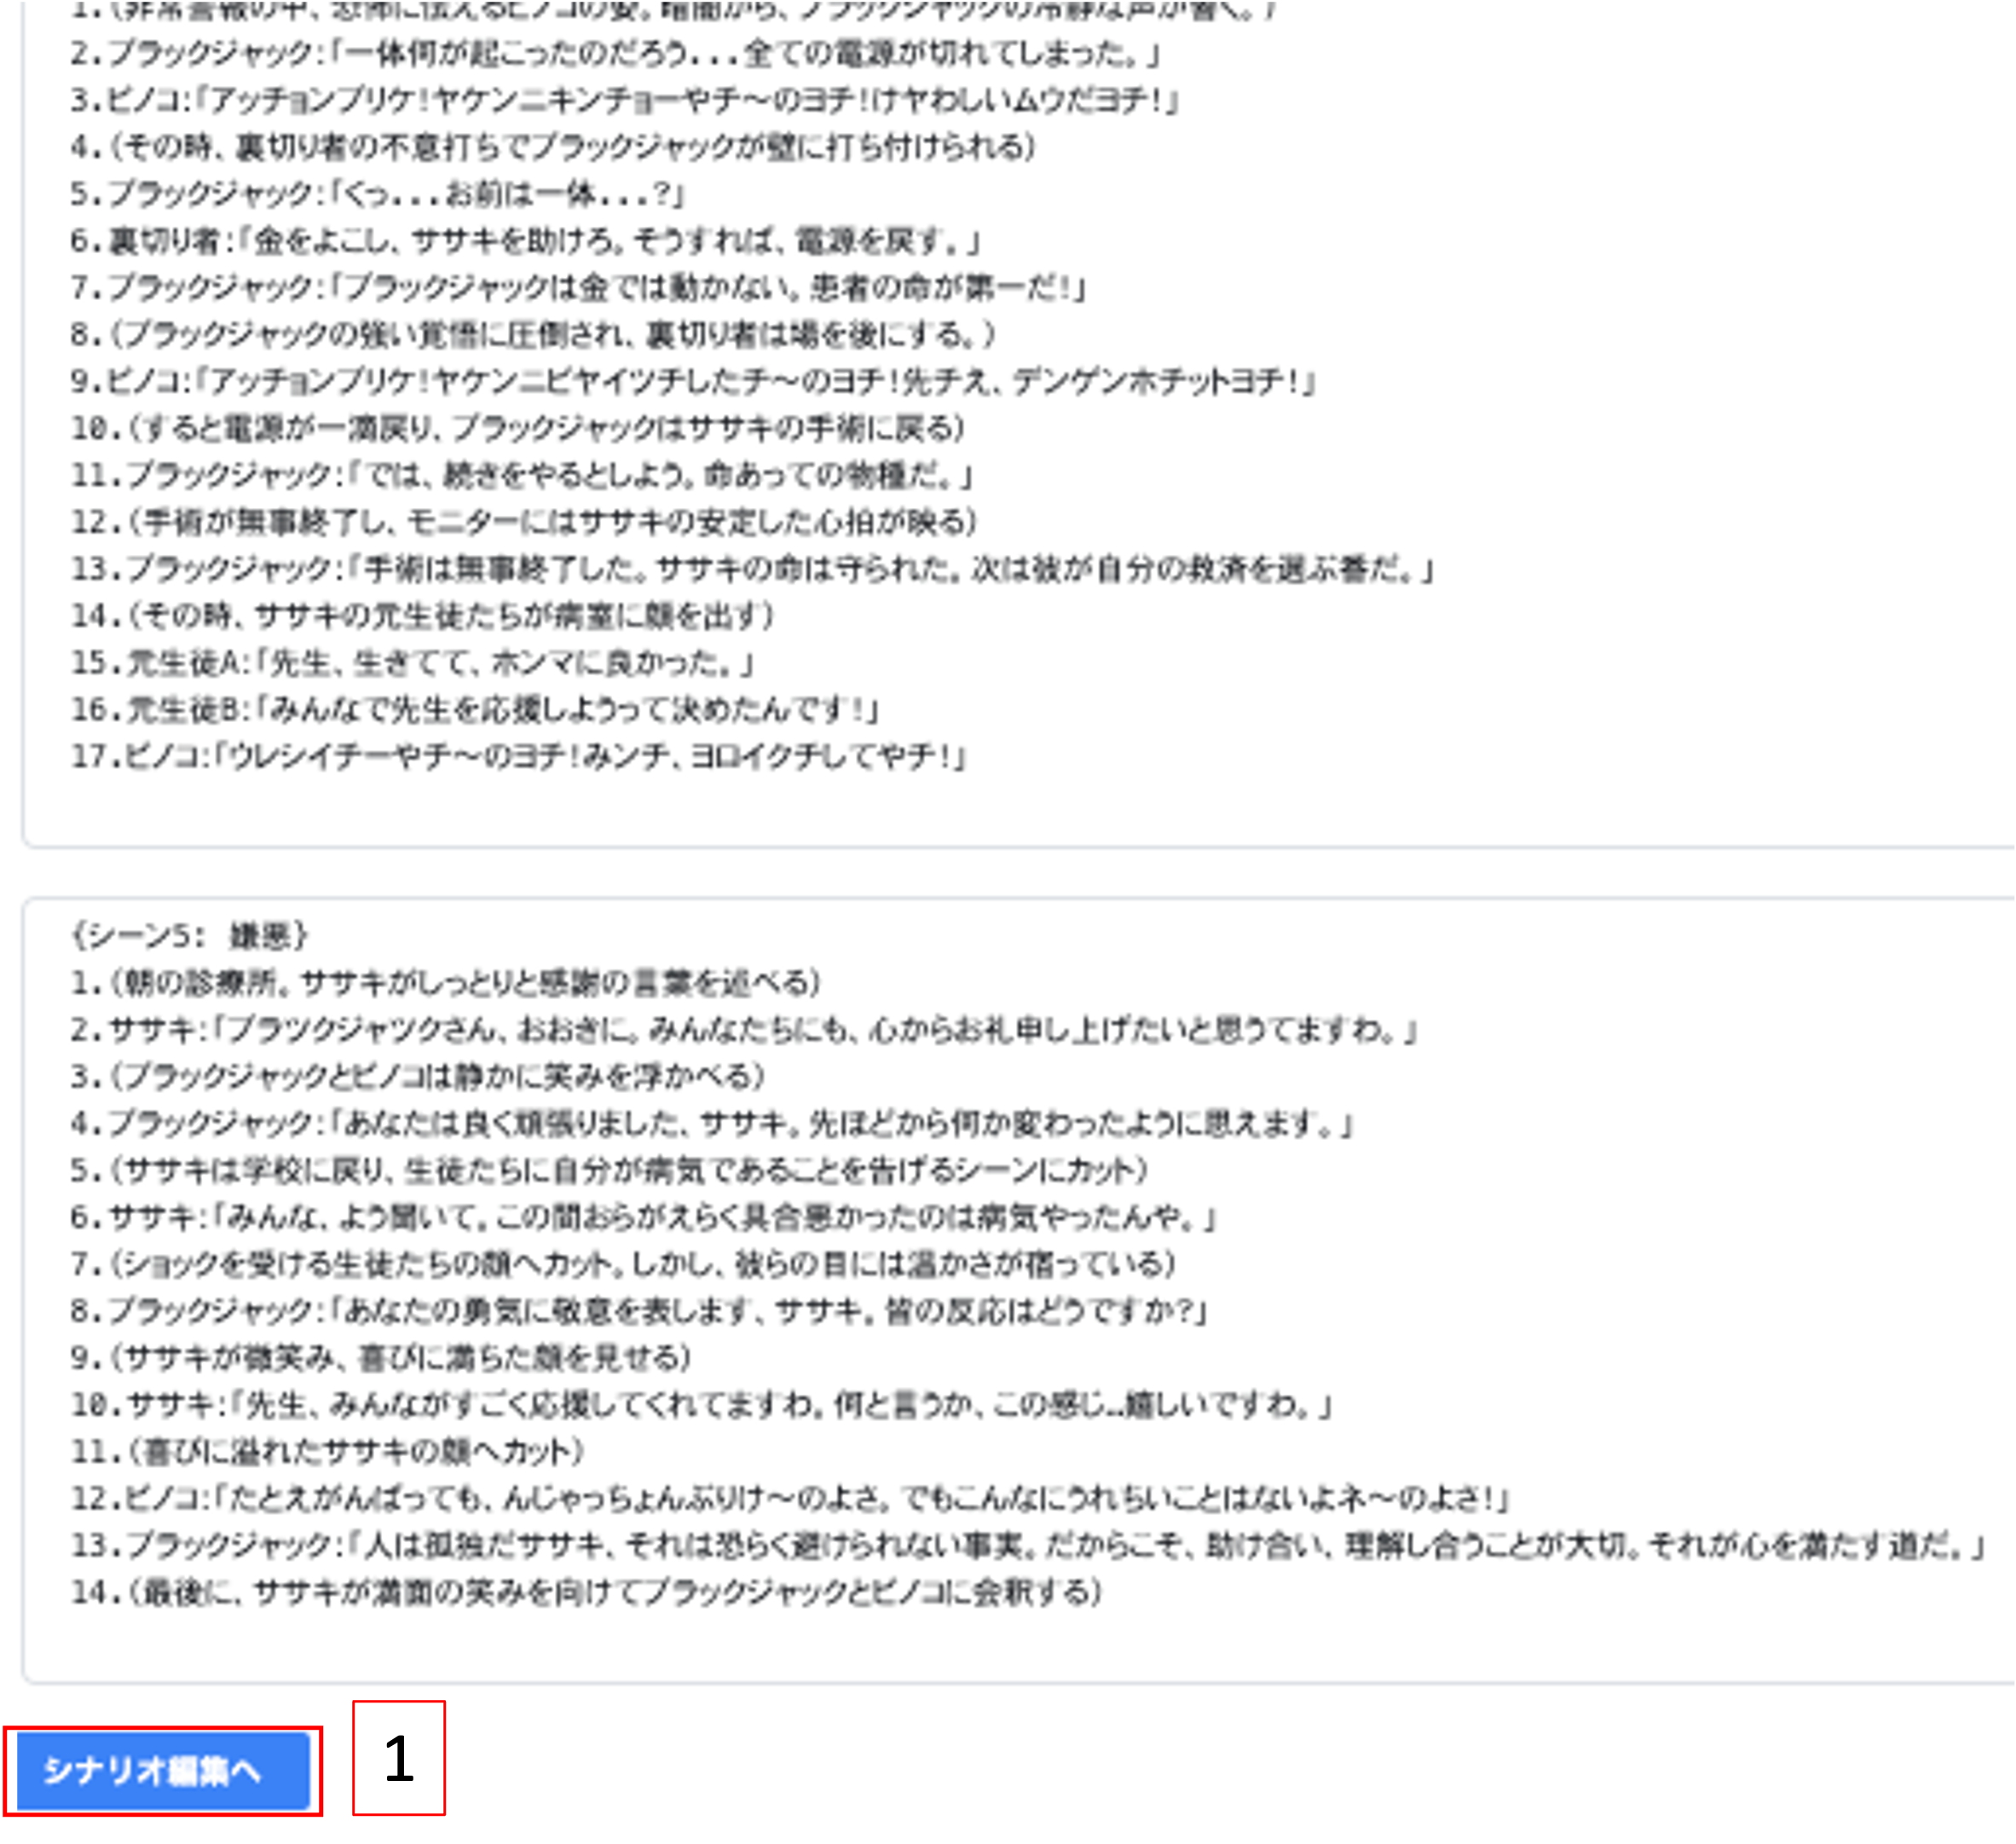
\includegraphics[width=12cm]{pict/04/scenario1_result.png}
   \caption[シナリオ生成機能1で生成されるシナリオの確認画面]{シナリオ生成機能1で生成されるシナリオの確認画面. \small (1): 「シナリオ編集へ」というボタンを押すと, シナリオ編集セクションへと移行する.}
   \label{scenario1_result}
   \end{center}
\end{figure}

\begin{breakitembox}
   [l]{シナリオ生成機能1で生成されるシナリオの例}
   {シーン1: 依頼}
1.（夜明け前、ブラックジャックの診療所の外観。突然、扉はガチャンと音を立てて開く）\\
2.ササキ：「おい、ブラックジャック君、まだ眠ってるんか。すまない、また付き合わせて」\\
3.（ササキがぎったない感じで笑う）\\
4.（ブラックジャックが驚きの表情を浮かべながら診療所の扉を開け、明るくササキに微笑んで見せる）\\
5.ブラックジャック：「久しぶりだねササキ、どうしてこんな時間に訪ねてきたのだ？」\\
6.（ササキの表情が急に険しくなり、彼が診療所に無言で入っていく）\\
7.（ブラックジャックが少し困惑した顔をしながら、彼についていく）\\
8.ブラックジャック：「何があったか、言ってみてくれ。」\\
9.（ササキが深く息を吸い込み、深刻そうにブラックジャックを見つめる）\\
10.ササキ：「どうもな、ちょっと俺、体の調子がおかしいんだわ。」\\
11.ピノコ：「たいしょあおかしいんの作？せんせぃ！ちゃあんと調べてみてちょうだいのよさ！アッチョンブリケ！」\\
12.（ブラックジャックがゆっくりとベッドに座り、ササキをじっと見つめる）\\
13.ブラックジャック：「もちろんだ、じっくりと検査してみよう。何でも話してくれ」\\
14.（ササキがため息をつきながら、ブラックジャックに自分のこぼれ話を始める。ササキの表情がだんだんと苦しみに満ちていく）\\
15.ピノコ：「せんせぃ、ちゃあんとリアチカルで優しく対応してちょうだいのよさ。」\\
\\
\\
{シーン2: 看病・治療}\\
1.（診察室でリハビリテーションの機器や治療ベッドの横でブラックジャックはササキの検査結果を見つめている）\\
2.ブラックジャック：「この病気は一般的な治療法では手に負えませんが、幸い私は対処法を知っています。」\\
3.ピノコ：「ほんとうに先生はよく知っているのよさ、一般の医者さんじゃダメだったのにさ。」\\
4.（ブラックジャックは強い意志を顔に出し、ピノコに向かって語りかける）\\
5.ブラックジャック：「ただ、治療だけでは足りない。彼の心のケアも必要だ。」\\
6.ピノコ：「心のケアも必要なんだ…。それってどういうことかな？」\\
7.ブラックジャック：「彼が病気で孤立してしまった原因も、人間関係の問題が大きい。だから心の問題を解決しなければ、病気の治療だけでは元気にはなれない」\\
8.（ササキがリハビリテーションを始め、ブラックジャックとピノコが見守っている）\\
9.ササキ：「ブラックジャックさん、本当にありがとう。一生懸命リハビリに励むわ。」\\
10.（シーンの最後に、ブラックジャックはササキのシャツの上から胸部を突き、ササキは苦しむ様子を見せる）\\
11.ブラックジャック：「これがあなたの病気のせいです。でも大丈夫、私たちはあなたを助けることができます。」\\
12.ピノコ：「アッチョンブリケ！先生、怖いこと言って驚かせないのよさ！でも、先生がいてくれて良かったのよさ。」\\
\\
{シーン3: 危機}\\
1.（ブラックジャックの診療所の手術室。ササキが手術台に横たわり、ブラックジャックは手術器具を手に持っている。ピノコが心配そうに見守っている。）\\
2.ブラックジャック：「何も心配するな、ササキ。全力で君を救おう。」\\
3.ササキ：「せんせえ、ホンマおおきに。ええ子やで。」\\
4.（しかし、その時、突如手術室の電源が落ち、全てが暗闇に包まれる。）\\
5.ピノコ：「アッチョンブリケ！でんきがちんまちたよさ！」\\
6.ブラックジャック：「何なんだ、この停電は！」\\
7.（電源が落ちると、手術を実行していた機器が全て停止し、ササキの命は一時的に危険な状態に。）\\
8.ブラックジャック：「手術が中断されるなんて、考えられない。ピノコ、手を貸してくれ！ハンドライトを持ってきてくれ」\\
9.ピノコ：「はいよさ、せんせい！」\\
10.（ブラックジャックは緊急状況に対応しようと、機転を利かせた行動を取り始める。一方で、病院内はパニックに。）\\
11.看護師A：「手術中の患者がいるのに、電源が！院長、何てこった！」\\
12.（ブラックジャックは状況を把握し、設備の復旧と安定した電力供給の確保に全力を傾け始める。一方、ササキは乱れる拍子を見つめながら、息を吹き返そうと努力している。）\\
13.ブラックジャック：「皆、落ち着け。このままでは患者を手術台に戻すことができない。復旧作業を急げ！」\\
14.ササキ：「こわいなあ、せんせえ。でも、がんばりまっせ。」\\
15.ピノコ：「ウソだよ、せんせい！ささきはがんばつているよさ！アッチョンブリケ」\\
16.ブラックジャック：「その甲斐あって、再開を待つだけだ。ササキ、我慢してくれ。」\\
\\
{シーン4: 依頼}\\
1.(非常警報の中、恐怖に怯えるピノコの姿。暗闇から、ブラックジャックの冷静な声が響く。)\\
2.ブラックジャック：「一体何が起こったのだろう...全ての電源が切れてしまった。」\\
3.ピノコ：「アッチョンブリケ！ヤケンニキンチョーやチ～のヨチ！けヤわしいムウだヨチ！」\\
4.（その時、裏切り者の不意打ちでブラックジャックが壁に打ち付けられる）\\
5.ブラックジャック：「くっ...お前は一体...？」\\
6.裏切り者：「金をよこし、ササキを助けろ。そうすれば、電源を戻す。」\\
7.ブラックジャック：「ブラックジャックは金では動かない。患者の命が第一だ！」\\
8.（ブラックジャックの強い覚悟に圧倒され、裏切り者は場を後にする。）\\
9.ピノコ：「アッチョンブリケ！ヤケンニビヤイツチしたチ～のヨチ！先チえ、デンゲンホチットヨチ！」\\
10.（すると電源が一滴戻り、ブラックジャックはササキの手術に戻る）\\
11.ブラックジャック：「では、続きをやるとしよう。命あっての物種だ。」\\
12.（手術が無事終了し、モニターにはササキの安定した心拍が映る）\\
13.ブラックジャック：「手術は無事終了した。ササキの命は守られた。次は彼が自分の救済を選ぶ番だ。」\\
14.（その時、ササキの元生徒たちが病室に顔を出す）\\
15.元生徒A：「先生、生きてて、ホンマに良かった。」\\
16.元生徒B：「みんなで先生を応援しようって決めたんです！」\\
17.ピノコ：「ウレシイチーやチ～のヨチ！みンチ、ヨロイクチしてやチ！」\\
\\
{シーン5: 嫌悪}\\
1.（朝の診療所。ササキがしっとりと感謝の言葉を述べる）\\
2.ササキ：「ブラツクジャツクさん、おおきに。みんなたちにも、心からお礼申し上げたいと思うてますわ。」\\
3.（ブラックジャックとピノコは静かに笑みを浮かべる）\\
4.ブラックジャック：「あなたは良く頑張りました、ササキ。先ほどから何か変わったように思えます。」\\
5.（ササキは学校に戻り、生徒たちに自分が病気であることを告げるシーンにカット）\\
6.ササキ：「みんな、よう聞いて。この間おらがえらく具合悪かったのは病気やったんや。」\\
7.（ショックを受ける生徒たちの顔へカット。しかし、彼らの目には温かさが宿っている）\\
8.ブラックジャック：「あなたの勇気に敬意を表します、ササキ。皆の反応はどうですか？」\\
9.（ササキが微笑み、喜びに満ちた顔を見せる）\\
10.ササキ：「先生、みんながすごく応援してくれてますわ。何と言うか、この感じ…嬉しいですわ。」\\
11.（喜びに溢れたササキの顔へカット）\\
12.ピノコ：「たとえがんばっても、んじゃっちょんぶりけ～のよさ。でもこんなにうれちいことはないよネ～のよさ！」\\
13.ブラックジャック：「人は孤独だササキ、それは恐らく避けられない事実。だからこそ、助け合い、理解し合うことが大切。それが心を満たす道だ。」\\
14.(最後に、ササキが満面の笑みを向けてブラックジャックとピノコに会釈する)
\end{breakitembox}
\vspace*{-7.5pt}
\begingroup
\captionof{figure}{シナリオ生成機能1で生成されるシナリオの例}
\label{scenario1_ex}
\endgroup

\subsection{シナリオ生成機能2}
本システムでは, シナリオ生成機能の一つとして, プロットから小説のような語り口の文章を生成させる機能も実装している. 

プロットから実際の漫画作品等へ作品を完成させていく過程において, 必要とされるのは具体性を持った表現である. その面においては, 小説のような語り口から得られる表現は有用であると考えられ, 本システムでは, このような表現を得るために, プロットから小説のような語り口の文章を生成させることができる機能を実装した. 

この機能を操作している様子を図\ref{scenario2}に示す. 操作は容易で, 図\ref{scenario2}に示した通り,「シナリオを生成」というボタンを押すことのみである. このような容易な操作により, プロットから小説のような語り口の文章を生成させることができるため, これはストーリークリエーターの創作支援に役立つものと考えられる.

結果が出力される画面は図\ref{scenario2_result}の通り. 生成結果が表示される画面はシナリオ生成機能1において生成結果を確認する画面と同様である.

小説のような語り口で表現された文章においても, シナリオ編集セクションにおいて編集することが可能である.

この機能で生成できる小説風の語り口の文章を図\ref{scenario2_ex}に示す.

\begin{figure}[H]
   \begin{center}
   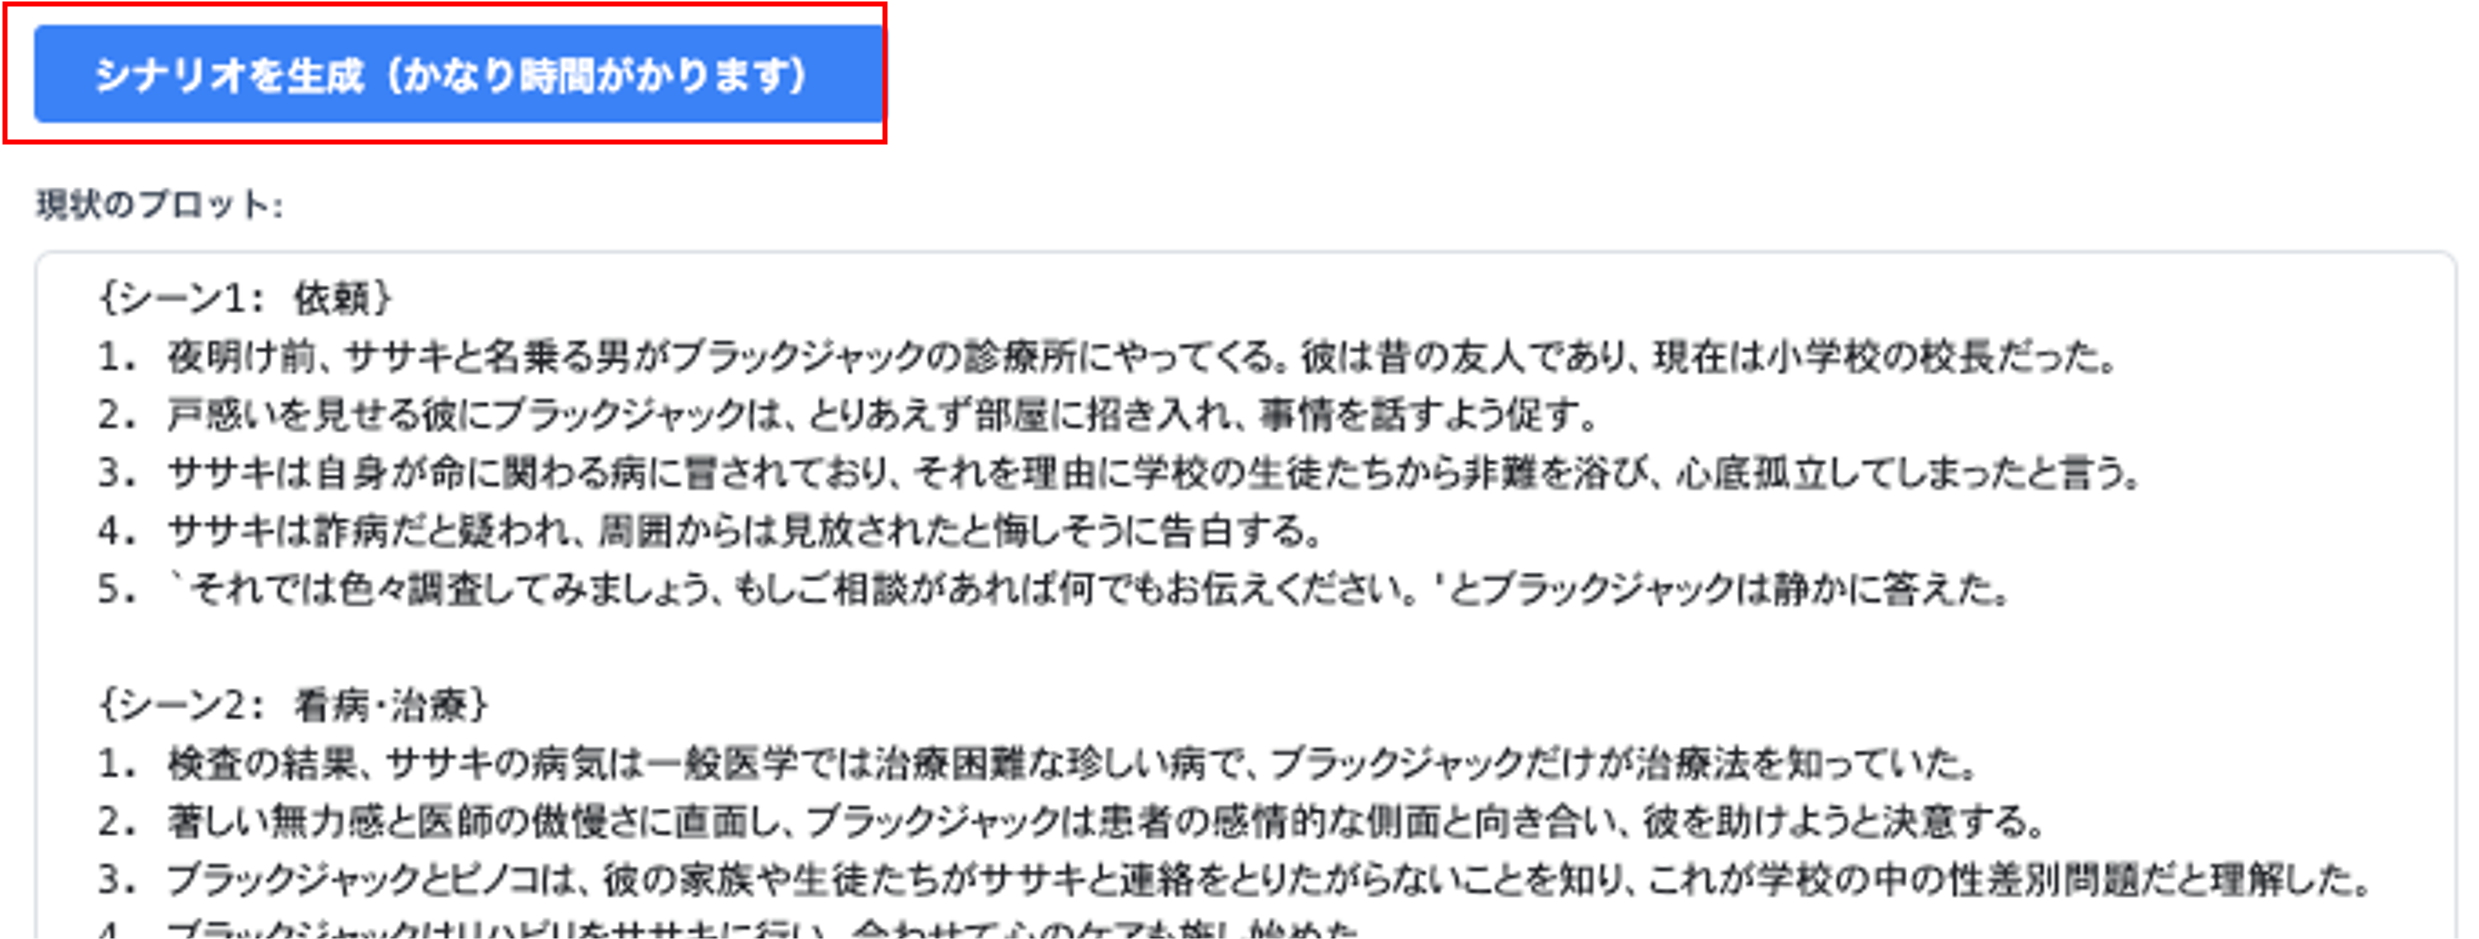
\includegraphics[width=12cm]{pict/04/scenario2.png}
   \caption[シナリオ生成機能2を実行する様子]{シナリオ生成機能2を実行する様子. \small (1): 「シナリオを生成」ボタンを押すと, LLMを介しプロットから小説のような語り口のシナリオが生成される.}
   \label{scenario2}
   \end{center}
\end{figure}

\begin{figure}[H]
   \begin{center}
   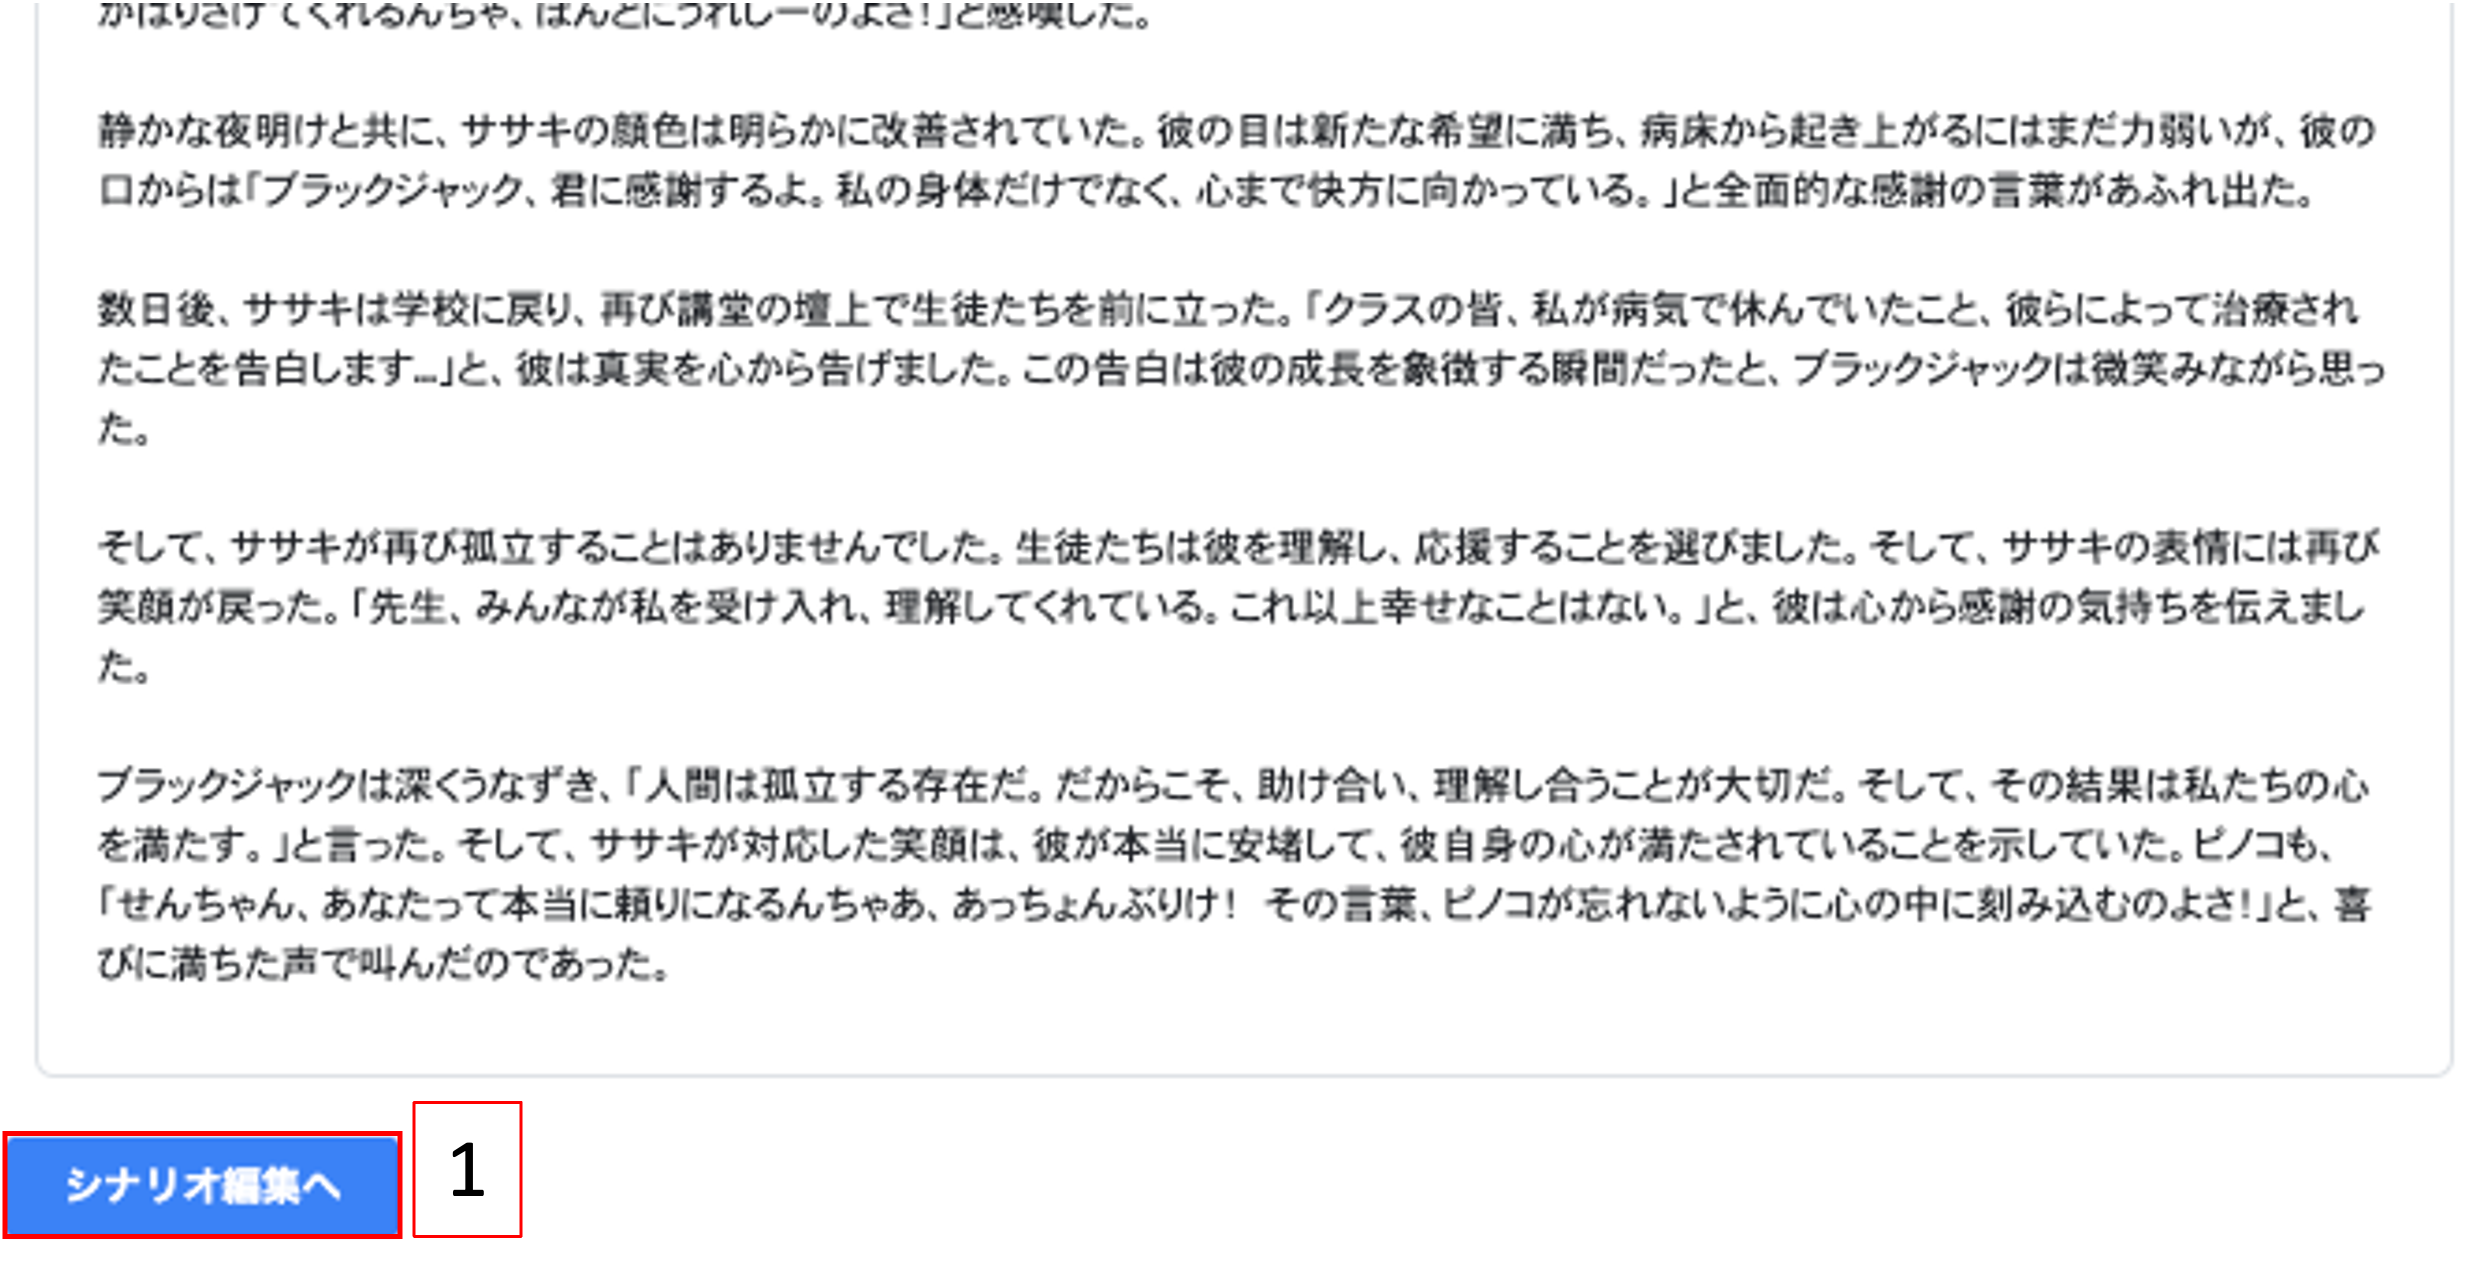
\includegraphics[width=12cm]{pict/04/scenario2_result.png}
   \caption[シナリオ生成機能2で生成されるシナリオの確認画面]{シナリオ生成機能2で生成されるシナリオ確認画面. \small (1): 「シナリオ編集へ」というボタンを押すと, シナリオ編集セクションへと移行する.}
   \label{scenario2_result}
   \end{center}
\end{figure}

\begin{breakitembox}
   [l]{シナリオ生成機能2で生成されるシナリオの例}
   夜が明ける僅か前、ほのかに月明かりが照らす診療所の扉をノックする音が響いた。そのドアを開けると、懐かしい顔をした男、ササキが立っていた。「昔、一緒に走り回った友人だ。現在は市立小学校で校長をしているんだ」とブラックジャックが口にした。\\
   \\
   見るからに混乱しているササキを、ブラックジャックは手際よく診察室に誘い入れる。「落ち着いて、何があったのか話してみ」と、彼の緊張を解くように言った。ササキの苦しげな表情が静寂を破った。彼の肩に手をかけ、「ボクがいて、なおさら孤独になったんだ。病に冒されたと知った生徒たちと教職員から突然に、あからさまに遠ざけられた。」と涙目になりながら告白した。\\
   \\
   「何も言わずに、ただ黙っているだけで、僕はうそつき呼ばわりされ、信用を無くした。」と、ササキは苦悩の表情を浮かべていた。「だから、僕はブラックジャックに来たんだ。真実を知りたい。そして、治療してほしいんだ」と、ササキはブラックジャックの目をまっすぐ見つめた。\\
   \\
   ブラックジャックは何も言わずに一瞥を投げただけだった。「では、こちらでいくつかテストをしてみましょう。何か問題があれば、どんな些細なことでもいいから伝えてください。」彼の声のトーンは穏やかで、安心感を与えてくれるものだった。\\
   \\
   ところで、その横では、ピノコが真剣な表情でササキを見つめていた。「せんちゃんもちっとかんしんをもつべきちゃ！ こんちゃくちゃなしぐさやことばをつかっちゃうんちゃあ！ アッチョンブリケ！ これがピノコの説教だってんこでも覚えておいてよさ！」と、彼女がブラックジャックに向けて強く語りかけていた。\\
   \\
   一連の診察と診断を経て、ササキは一般医学では対処困難な稀な疾患であることが発覚した。その答えを見つけ出せたのはブラックジャックだけだった。彼は自宅でピノコと一緒にササキの病歴と結果を慎重に分析し、「この疾患は最新の治療法で治療することが可能だ、だがそれには時間と忍耐が必要だぞ」と告げた。\\
   \\
   ブラックジャックのその言葉を聞き、ササキは始めて希望の光を見つけた。「私を救ってくれるのですか？」と彼は疑うような表情で尋ねた。「当然だ、だが君がそれを望むなら、私たちは一緒に闘わなければならない。君が今、一人だけで抱え込んでいる心の問題も解決しなければならない。」とブラックジャックは真面目な顔をしてササキに語りかけた。\\
   \\
   次に、ブラックジャックとピノコがササキの家族や生徒たちと接触した際、彼らがササキから避け続けていることを確認した。そして、ブラックジャックとピノコは、これが学校内に広がるジェンダーバイアスによる結果だと推測した。「こりゃあ、大したないちゃいちゃいクンとちゃいちゃいメタンとのまちがいだんちゃあ！ アッチョンブリケ！ 先生、ほんとにあんなちょわんちゃんたちをしょうかいちょうかしてあげるべきちゃあ。」と、ピノコはブラックジャックに彼らを指差して庇護を乞うように主張した。\\
   \\
   すぐさま、ブラックジャックはリハビリテーションの予定を立て、ササキの心のケアを開始した。リハビリの過程で、彼はササキに自己信頼を回復するための支援を提供し、そして、ササキの心の回復に心を砕いて働いた。\\
   \\
   そこに深い共感を覚え、ブラックジャックは誓った。「君の心の傷も僕が治してみせる。そして、君が再び自信を取り戻せるように、僕が全力を尽くす。だから、諦めるな。君を見捨てることはない。」この時、ブラックジャックは眼前の男が持つ努力と闘争心に激励され、ササキと共にこの闘いに立ち向かう事を誓ったのだった。\\
   \\
   見舞いの途中で、突如としてササキの身体が堪えきれなくなり、倒れてしまった。彼の顔色は灰色に変わり、息も荒くなっていた。その瞬間、ブラックジャックは全てをほったらかしてササキのもとへ駆け寄り、彼を即座に手術台に乗せた。\\
   \\
   院内には緊迫した静寂が広がり、ブラックジャックは手術の準備に取り掛かった。ピノコも赤いチュニックの袖をまくり上げて、「せんちゃん、さかんにするんちゃあ！ ピノコと手とてようにしただのよさ！」と強く叫んだ。\\
   \\
   しかし、手術が始まろうとするその瞬間、突然全ての電源が切れてしまった。松明のような非常灯だけが暗い手術室を照らし、緊迫感は最高潮に達した。「先生、こんなトラブルが起こるなんてどうするのよさ？」と、ピノコが叫んだ。\\
   \\
   手術は自らの最大限の努力を尽くし、ブラックジャックはその突発事態を解決するために駆け回っていた。その一方で、中断された手術の結果、ササキの心拍数は急に減少し始めた。彼の生命の火は揺らぎ、死にかけているように見えた。\\
   \\
   「くそっ、何者だ、こんなことをしたのは。おれが直ちに解決する、待っていてくれ、ササキ」ブラックジャックは敵意を露わにして叫んだ。その間も、ピノコは細い肩を震わせ、不安そうにブラックジャックを見つめていた。「先生、ひゃくぱあほねっとが足りないのよさ！ アッチョンブリケなんちゃあ！」と、言葉を詰まらせて叫んだ。\\
   \\
   電源の問題が起きた原因は遂に判明した。それは、ササキの敵で病院内の裏切り者による仕業だった。彼は莫大な報酬を要求し、ブラックジャックに半ば脅しのように「ササキを助けるためには、私に金を渡しなさい。」と言った。\\
   \\
   しかしながら、ブラックジャックはその要求に屈すること無く、無視して電源の修復に全神経を注いだ。「お前の認識が間違っている、ここでやるべき仕事は医者の仕事だ。患者を救うために全力を尽くすべきだ。」と彼は胸を張って言った。\\
   \\
   ブラックジャックの揺るぎない決意の前に、裏切り者は立ち去った。電源がすぐに復旧し、手術は再開。最終的に、ササキの処置は順調に行われ、彼は危険な状況から救われた。\\
   \\
   その後、気分が晴れたササキの元には元生徒たちが次々と訪れ、心からの謝罪を述べ、和解を進めてゆきました。「先生、ごめんなさい。やっと本当のことを理解できました。」と彼らは白状し、ササキは元校長としての威厳を取り戻した。\\
   \\
   一方ブラックジャックはその結果に満足した。「それが君にとっての正解だ、ササキ。君が信頼していた皆に、君の存在の大切さを再認識させることができた。」と彼は本心から言った。ピノコも「せんちゃんのやさしかとちゃよかとちゃあ！ ひとりぼっちになったササキちゃんをみんながはりさげてくれるんちゃ、ほんとにうれしーのよさ！」と感嘆した。\\
   \\
   静かな夜明けと共に、ササキの顔色は明らかに改善されていた。彼の目は新たな希望に満ち、病床から起き上がるにはまだ力弱いが、彼の口からは「ブラックジャック、君に感謝するよ。私の身体だけでなく、心まで快方に向かっている。」と全面的な感謝の言葉があふれ出た。\\
   \\
   数日後、ササキは学校に戻り、再び講堂の壇上で生徒たちを前に立った。「クラスの皆、私が病気で休んでいたこと、彼らによって治療されたことを告白します…」と、彼は真実を心から告げました。この告白は彼の成長を象徴する瞬間だったと、ブラックジャックは微笑みながら思った。\\
   \\
   そして、ササキが再び孤立することはありませんでした。生徒たちは彼を理解し、応援することを選びました。そして、ササキの表情には再び笑顔が戻った。「先生、みんなが私を受け入れ、理解してくれている。これ以上幸せなことはない。」と、彼は心から感謝の気持ちを伝えました。\\
   \\
   ブラックジャックは深くうなずき、「人間は孤立する存在だ。だからこそ、助け合い、理解し合うことが大切だ。そして、その結果は私たちの心を満たす。」と言った。そして、ササキが対応した笑顔は、彼が本当に安堵して、彼自身の心が満たされていることを示していた。ピノコも、「せんちゃん、あなたって本当に頼りになるんちゃあ、あっちょんぶりけ！ その言葉、ピノコが忘れないように心の中に刻み込むのよさ！」と、喜びに満ちた声で叫んだのであった。
\end{breakitembox}
\begingroup
\captionof{figure}{シナリオ生成機能2で生成されるシナリオの例}
\label{scenario2_ex}
\endgroup

\section{シナリオ編集セクション}\label{sec: scenario_edit}
ここでは, プロット編集セクション同様, 生成したシナリオに対して編集機能を適用することができるシナリオ編集セクションについて説明する. 

このセクションにおけるフローは, プロット編集セクションと変わない. 編集機能を適用すると, 適用後のシナリオと既存のシナリオを比較することができる画面へと遷移し, 満足のいく方を残すことができる. これを繰り返し行なっていくことで, ユーザーにとって満足のいくシナリオへと改善していくことができる. 実装した編集機能の一覧は以下の通り. ここで実装した機能の多くはプロット編集セクションと同じものを利用しているが, シナリオに対し適用するには不自然であると考えられる機能は実装していない. それとは反対に, プロット編集セクションにはなく, シナリオ編集セクションにおいてのみ利用可能な機能, 登場人物の口調変更機能を実装した. 以下では, シナリオ編集セクション特有の登場人物の口調変更機能について説明する.

\begin{itemize}
   \item フリーワードによるやり取り
   \item シナリオ中の単語・文章に関する質問
   \item アイデア生成
   \item 伏線の処理
   \item 一部シーン変更
   \item 全体的な雰囲気の変更
   \item シナリオの部分修正
   \item 不自然な日本語の修正
   \item 手作業での編集
   \item \hyperref[subsec:line_edit]{登場人物の口調変更}
\end{itemize}

\subsection{登場人物の口調変更}\label{subsec:line_edit}
登場人物が発する台詞は, 物語の重要な要素の一つである. 特にシナリオは台詞を中心とした文章であるためその重要度は大きい. Mirowskiら\cite{mirowski23}の研究においても, 物語を登場人物たちの対話へと収束させるようシステムを構築している. そのため, 本システムでも登場人物の台詞の重要性を鑑み, 台詞の口調を変更する機能を実装した. この機能は, 登場人物ごとに口調を設定することで, 物語としての筋を変えることなくシナリオ上での各登場人物の台詞回しを変更することができる機能である. クリエーターが登場人物に対しこうあってほしいというイメージをもちつつもその具体案に苦慮している場合, そのイメージを実現するために利用することができる. また, この機能を利用することで, 登場人物の個性をより強く表現することができると考えられる.

登場人物の口調変更機能を操作している様子を図\ref{line_edit}に示す. 操作は容易で, 図\ref{line_edit}に示した通り, テキストエリアへの入力とボタンを押すだけで口調が変更されたシナリオを得ることができる. 生成されたシナリオ図\ref{line_edit_result}の通り, 既存のシナリオと編集機能適用後のシナリオを比較する画面で確認することができ, ここで満足のいく方を残し, 再びシナリオ編集機能を適用することもできる.

物語の重要な要素の一つである台詞を, イメージから具体化する方法として働き, クリエーターの創作を支援する.

\begin{figure}
   \begin{center}
   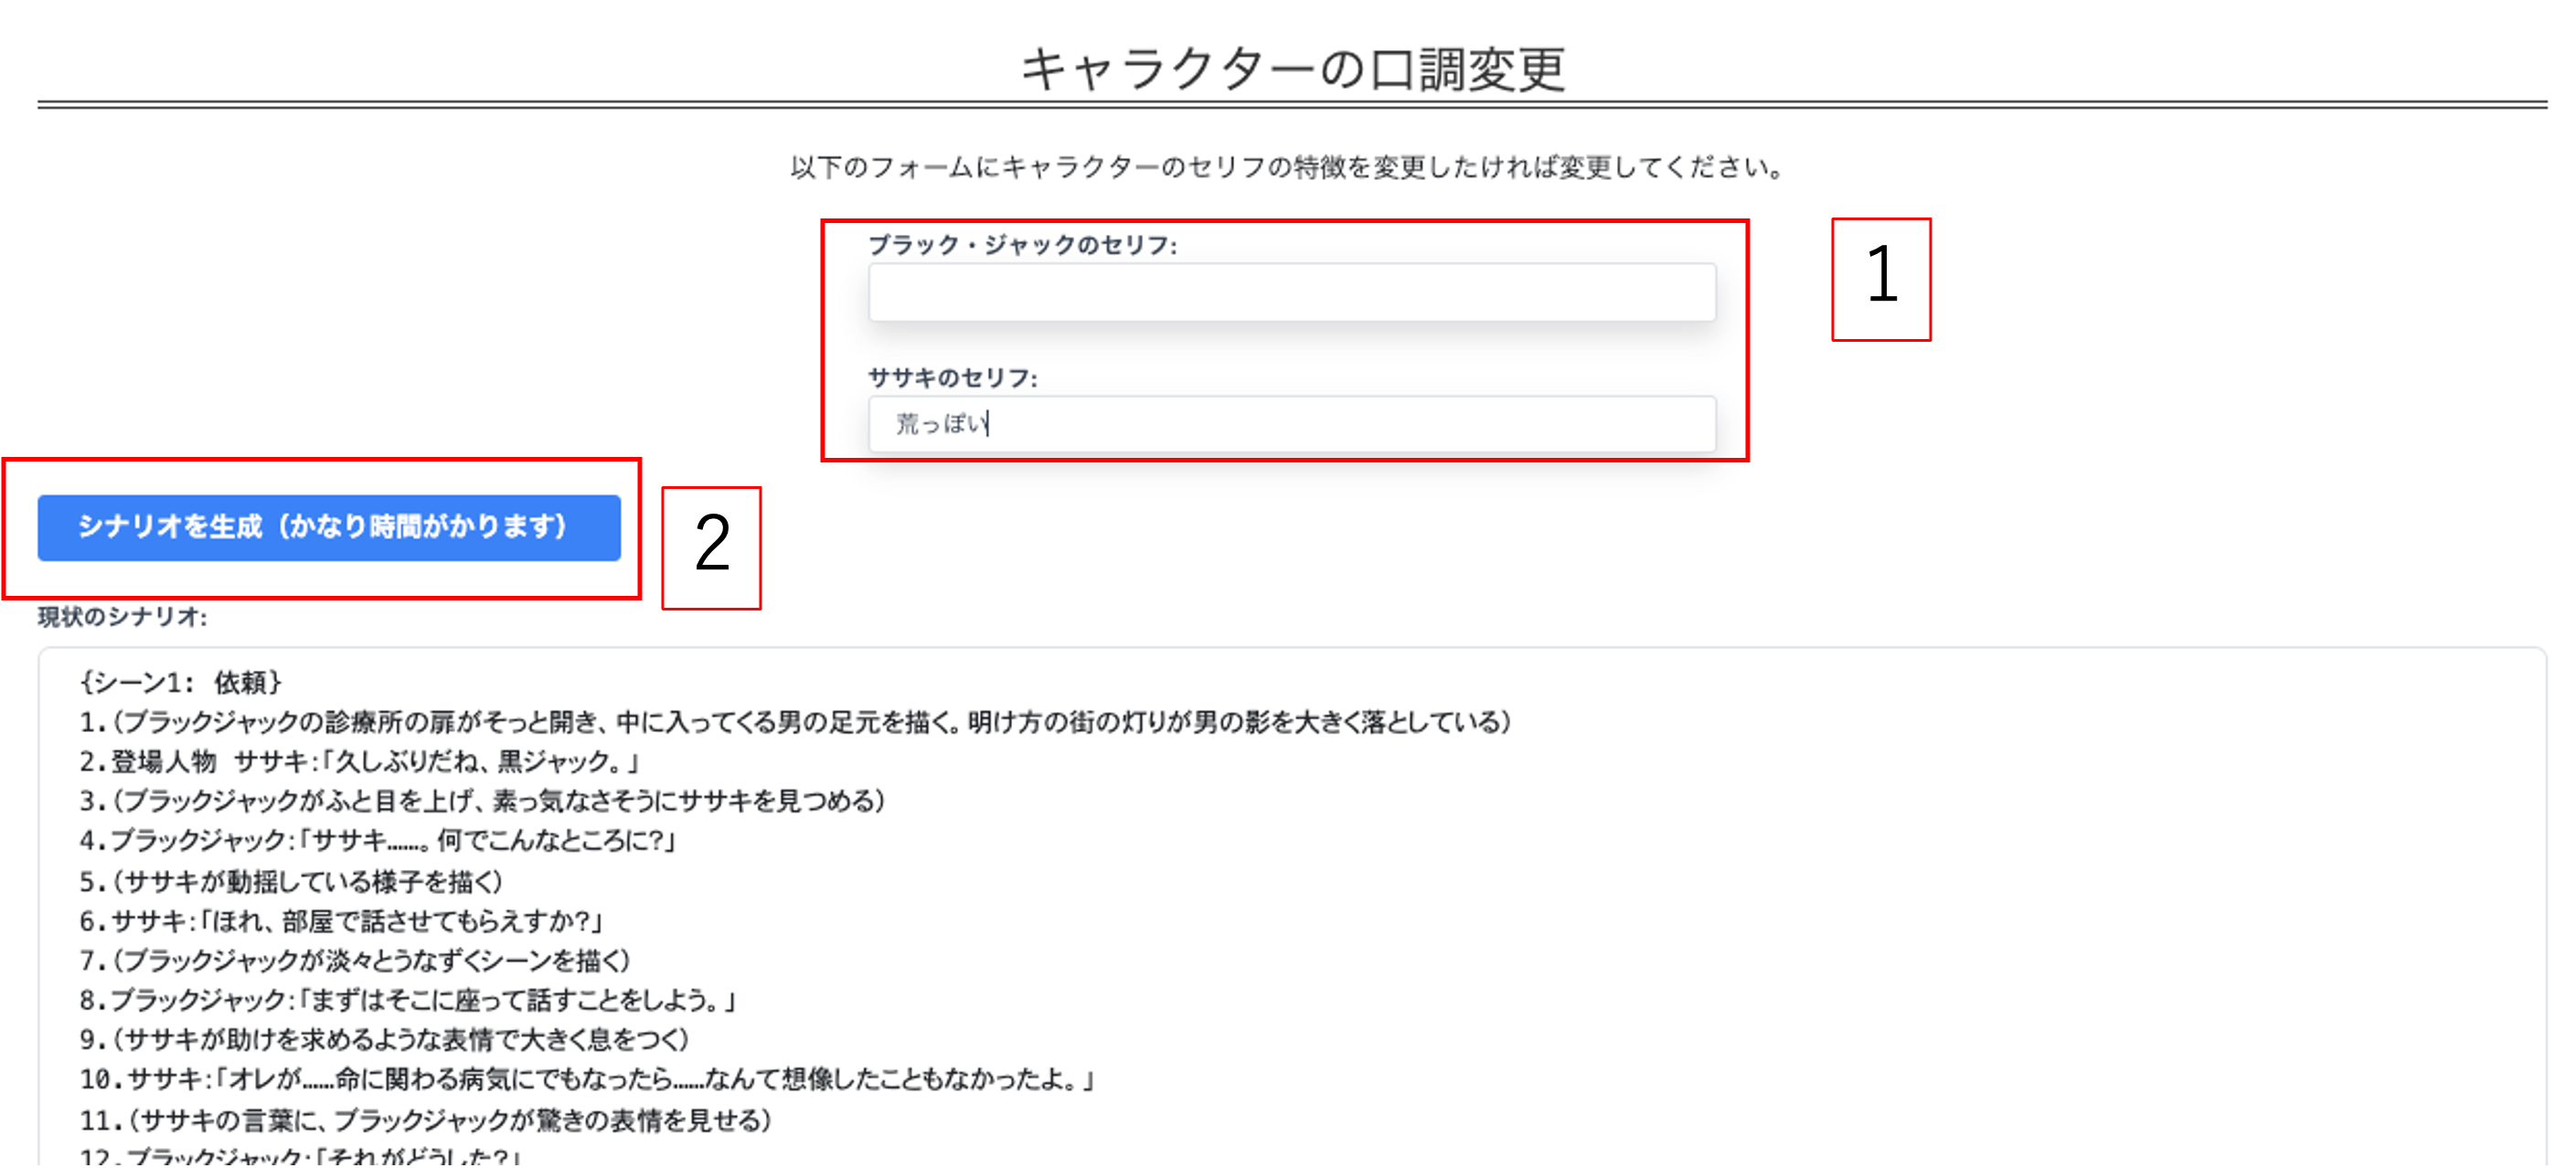
\includegraphics[width=12cm]{pict/04/line_edit.png}
   \caption[登場人物の口調変更機能を実行する様子]{登場人物の口調変更機能を実行する様子. \small (1): 口調を変更したい登場人物のテキストエリアで口調を指定. (2): 「シナリオ生成」ボタンを押すと, LLMを介しプロットからシナリオが生成される.}
   \label{line_edit}
   \end{center}
\end{figure}

\begin{figure}
   \begin{center}
   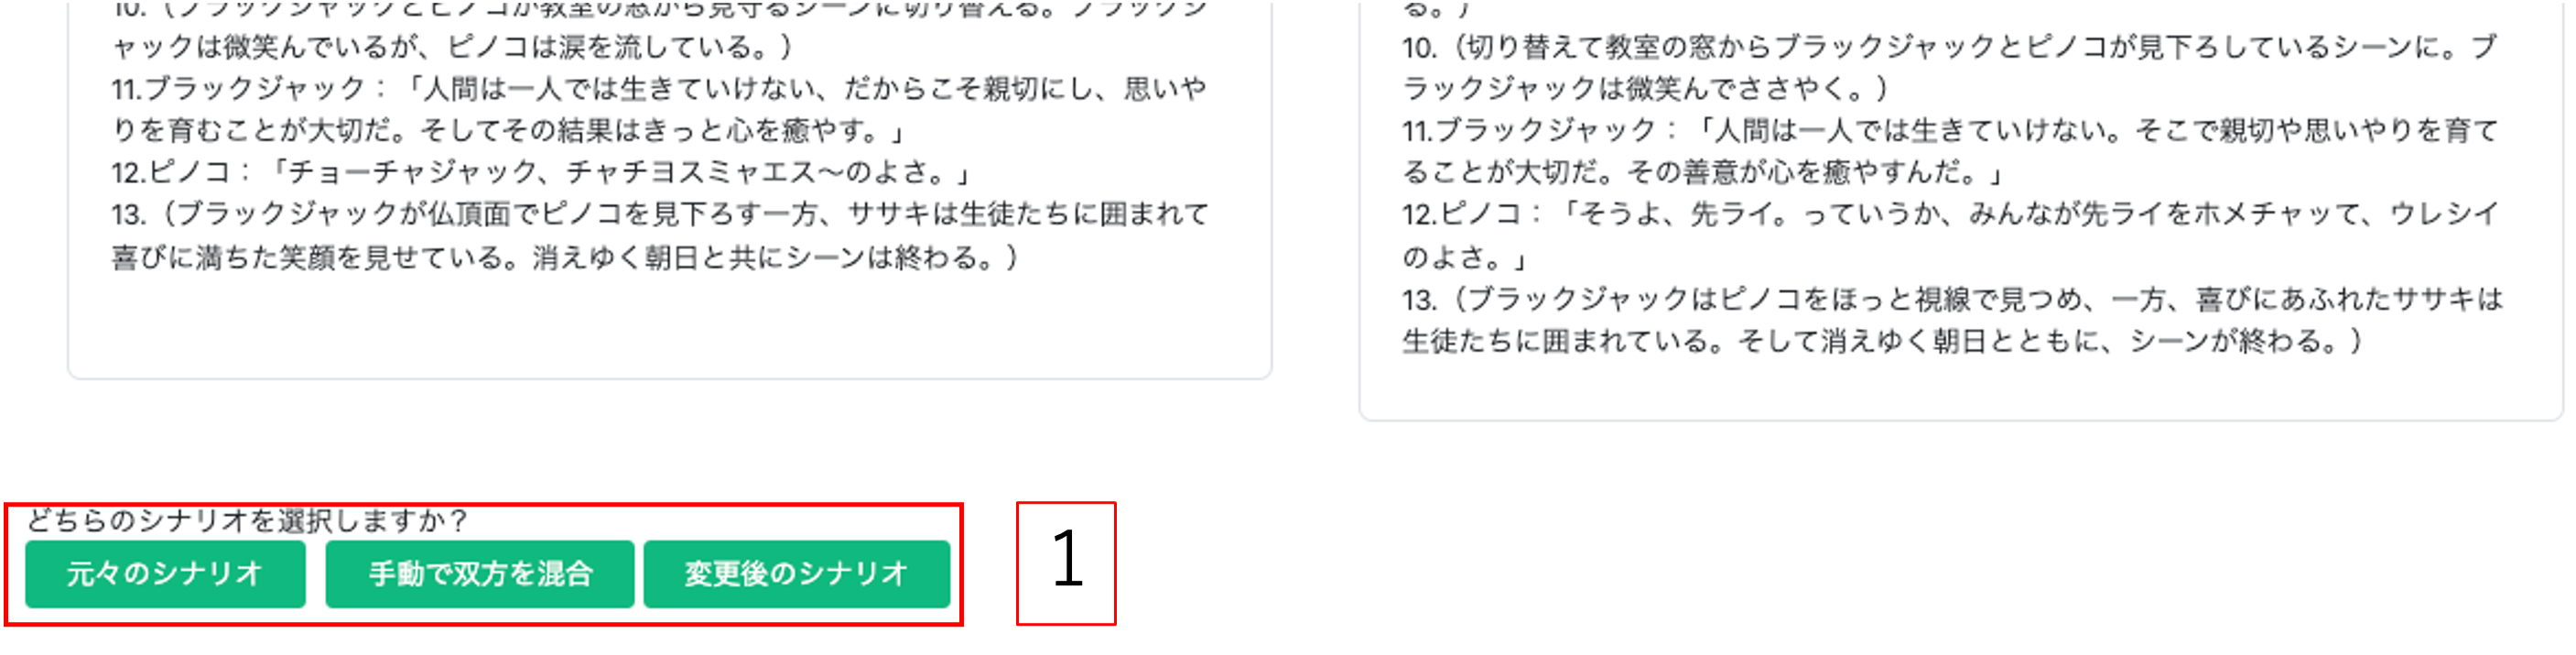
\includegraphics[width=12cm]{pict/04/line_edit_result.png}
   \caption[シナリオ編集機能適用後の比較画面]{シナリオ編集機能適用後の比較画面. \small (1):「元々のシナリオ」「手動で双方を混合」「変更後のシナリオ」のいずれかのボタンを押すことで, 満足のいく方を残すことができる.}
   \label{line_edit_result}
   \end{center}
\end{figure}

\section{実装}\label{sec:implementation}
本システムの開発に際し, 筆者が実装に関わった機能をここに列挙する.

\begin{itemize}
   \item \hyperref[subsec: freeword]{フリーワードによるやり取り}
   \item \hyperref[subsec: question]{プロット中の単語・文章に関する質問}
   \item \hyperref[subsec: idea]{アイデア生成}
   \item \hyperref[subsec: comparison]{新旧プロットの比較}
   \item \hyperref[sec: scenario_generation]{シナリオ生成セクション}   
   \item \hyperref[sec: scenario_edit]{シナリオ編集セクション}
\end{itemize}

実装に際し, 次の点に留意した. GPT-4 の API では, 一度に送信できるテキストの量に制限がある. このシステムで扱われるテキストは, ときに拡張されたプロットやシナリオなどでこの制限にかかってしまう. シーンごとに分割するなどしてこの問題に対処した. 

もちろん本システムは筆者だけの力で完成したものではなく, そのようなことを妄言するつもりもないということを固く留めておかれたい.


\expandafter\ifx\csname ifdraft\endcsname\relax
   \fancyhead[LO]{}
   \printbibliography[title=参考文献]
   \end{document}
   \fancyhead[LO]{\rightmark}
   \fi